\documentclass[10pt,a4paper,openany]{report}

\usepackage[utf8]{inputenc}
\usepackage[T1]{fontenc}
\usepackage{palatino}
\usepackage{microtype}
\usepackage{amsmath,amssymb,amsthm}
\usepackage{mathtools}
\usepackage{bm} % <-- ADDED: For bold math symbols (vectors, matrices) used in Ch05 & Ch06
\usepackage{booktabs}
\usepackage{geometry}
\usepackage{xcolor}
\usepackage{graphicx} % <-- ADDED: Crucial for inserting real images later
\usepackage{float}    % <-- ADDED: For precise figure placement [H]
\usepackage{titlesec}
\usepackage{enumitem}
\usepackage{array}
\usepackage{tabularx}
\usepackage{fancyhdr}
\usepackage{tikz}
\usetikzlibrary{arrows.meta,positioning,shapes.geometric,shapes.misc,
  calc,decorations.pathreplacing,fit,backgrounds,matrix,decorations.markings}
\usepackage{pgfplots}
\pgfplotsset{compat=1.18}
\usepackage[many]{tcolorbox}
\usepackage{hyperref}

% ── geometry ─────────────────────────────────────────────────────────
\geometry{top=2.2cm,bottom=2.2cm,left=2.4cm,right=2.4cm,headheight=13pt}

% ── headers ──────────────────────────────────────────────────────────
\pagestyle{fancy}\fancyhf{}
\fancyhead[LO]{\nouppercase{\rightmark}}
\fancyhead[RE]{\nouppercase{\leftmark}}
\fancyhead[LE,RO]{\thepage}
\renewcommand{\headrulewidth}{0.4pt}

% ── chapter/section titles (GRAYSCALE & FIXED) ───────────────────────
\titleformat{\chapter}[display]
  {\normalfont\bfseries\color{black}}
  {\filleft\large Chapter~\thechapter}{1ex}
  {\titlerule[1pt]\vspace{1ex}\filright\LARGE}
  [{\vspace{1ex}\titlerule[1pt]}]

\titleformat{\section}
  {\normalfont\large\bfseries\color{black}}
  {\thesection}{1em}{}
  [{\titlerule[0.4pt]}]

\titleformat{\subsection}
  {\normalfont\normalsize\bfseries\color{black}}
  {\thesubsection}{1em}{}

% ── tcolorboxes (GRAYSCALE) ──────────────────────────────────────────
\newtcolorbox{insightbox}[1][]{enhanced,breakable,
  colback=white,colframe=black,
  fonttitle=\bfseries\small,title={Key Insight\ifx&#1&\else: #1\fi},
  boxrule=1pt,arc=3pt,drop fuzzy shadow=black!20,left=7pt,right=7pt,top=3pt,bottom=3pt}

\newtcolorbox{mathbox}[1][]{enhanced,breakable,
  colback=black!3,colframe=black,
  fonttitle=\bfseries\small,title={Derivation\ifx&#1&\else: #1\fi},
  boxrule=1pt,arc=3pt,left=7pt,right=7pt,top=3pt,bottom=3pt}

\newtcolorbox{warningbox}[1][]{enhanced,breakable,
  colback=black!5,colframe=black,
  fonttitle=\bfseries\small,title={Watch out\ifx&#1&\else: #1\fi},
  boxrule=1pt,arc=3pt,left=7pt,right=7pt,top=3pt,bottom=3pt}

\newtcolorbox{defbox}[1][]{enhanced,breakable,
  colback=white,colframe=black,
  fonttitle=\bfseries\small,title={Definition\ifx&#1&\else: #1\fi},
  boxrule=1pt,arc=3pt,left=7pt,right=7pt,top=3pt,bottom=3pt}

% image placeholder
\newcommand{\figplaceholder}[2]{%
  \begin{center}
  \begin{tikzpicture}
    \draw[dashed,gray!60,thick,rounded corners=4pt]
      (0,0) rectangle (12cm,3.8cm);
    \node[gray!70,font=\small\itshape,align=center] at (6cm,1.9cm)
      {$\blacksquare$\quad #1\\[4pt]\footnotesize #2};
  \end{tikzpicture}
  \end{center}}

% ── macros ───────────────────────────────────────────────────────────
\newcommand{\R}{\mathbb{R}}
\newcommand{\e}{\mathrm{e}}
\newcommand{\ddt}{\frac{d}{dt}}
\newcommand{\ppt}{\frac{\partial}{\partial t}}
\newcommand{\ppx}{\frac{\partial}{\partial x}}

% ── theorems ─────────────────────────────────────────────────────────
\theoremstyle{definition}
\newtheorem{example}{Example}[chapter]
\theoremstyle{remark}
\newtheorem{remark}{Remark}[chapter]

% ── hyperref (GRAYSCALE) ─────────────────────────────────────────────
\hypersetup{colorlinks,linkcolor=black,urlcolor=black,
  pdftitle={Modelling and Simulation of Mechatronic Systems -- Study Notes}}

%══════════════════════════════════════════════════════════════════════
\begin{document}
%══════════════════════════════════════════════════════════════════════

\title{\vspace{-1cm}
  \LARGE\bfseries Modelling and Simulation\\of Mechatronic Systems\\[0.5cm]
  \large\normalfont\itshape Complete Study Notes\\[0.3cm]
  \normalsize\textcolor{gray}{Based on A.~Macchelli's lectures --- UniBO DISI}}
\author{Study Notes}
\date{\today}
\maketitle\thispagestyle{empty}

\tableofcontents\newpage

%──────────────────────────────────────────────────────────────────────
\part{Foundations of Bond Graph Modelling}
%──────────────────────────────────────────────────────────────────────
 %══════════════════════════════════════════════════════════════════════
\chapter{Physical Modelling and the Bond Graph Philosophy}
%══════════════════════════════════════════════════════════════════════

The goal of this course is to build \textbf{mathematical models of dynamic mechatronic systems} — systems that combine mechanics, electronics, hydraulics and thermodynamics into a single interacting whole[cite: 1].
The challenge is that each of these domains has historically developed its own graphical notation and set of equations (circuit diagrams, free-body diagrams, hydraulic schematics), which makes multi-domain systems hard to model coherently[cite: 2].
\textbf{Bond graph theory} solves this by providing a single, unified, energy-based language that describes all physical domains on the same footing[cite: 3].
This uniform notation allows one to study the structure of the system, meaning the nature of the parts and the sets of interconnections among them[cite: 120, 121].

\section{The systems viewpoint}

A \textbf{system} is any entity that can be conceptually separated from its environment by a physical or conceptual boundary[cite: 4, 72].
Inside the boundary are interacting subsystems and components; across the boundary flow the stimuli (inputs) and responses (outputs)[cite: 5].
The key insight of the systems viewpoint is that a system's behaviour \emph{as a whole} is not simply the superposition of its parts in isolation — interfaces and interactions matter just as much as individual component dynamics[cite: 6, 84].
In engineering practice, design tasks are broken into parts worked on in isolation, but those parts must ultimately interact[cite: 7, 81].
If the assumptions made in one group are too crude, the assembled system fails to meet its specification[cite: 8].
The systems engineer must hold both the component detail and the system-level behaviour in view simultaneously[cite: 9]. 
Achieving this ideal goal requires knowledge pertinent to the study of systems per se, bridging isolated disciplines like vibrations, dynamics, fluid mechanics, thermo-dynamics, and automatic control[cite: 92, 93, 94, 95, 96, 97].

\begin{insightbox}[The modelling trade-off]
No system can be modelled exactly. The art is to choose the \textbf{right level of complexity}: detailed enough to answer the questions being asked, simple enough to be tractable[cite: 10, 74].
A model that is too simple will miss important dynamics[cite: 11];
one that is too detailed will obscure the physics and be computationally intractable[cite: 12].
This judgement is acquired through practice and physical intuition[cite: 13].
\end{insightbox}

Dynamic models serve four distinct purposes: 
\begin{itemize}
    \item \textbf{Analysis}: Predict the future given known inputs and initial conditions[cite: 14]. This can be data-based (black box) or physics-law based (white box) depending on how the component is characterized[cite: 201, 212, 214].
    \item \textbf{Identification}: Find the model from measured input/output histories[cite: 14].
    \item \textbf{Synthesis}: Find the system that turns a given input into a desired output[cite: 14].
    \item \textbf{Control}: Design a feedback law that drives the system to a desired behaviour[cite: 14].
\end{itemize}
Each task uses the same model but in a different way[cite: 14].

\section{Power as the universal currency}

The central idea of bond graph theory is that \textbf{all physical interactions involve the exchange of power}[cite: 15, 229].
When a motor drives a pump, when a spring pushes a mass, when a voltage source drives a current through a resistor — in every case, energy flows across a boundary, and the instantaneous rate of that flow is power[cite: 16].
By making power the primary language, bond graphs work equally well in every energy domain[cite: 17].
At every interconnection point between subsystems — called a \textbf{port} — two variables are defined whose product is instantaneous power:
\begin{equation}
  P(t) = e(t)\,f(t)
\end{equation}
These are called the \textbf{effort} $e$ and the \textbf{flow} $f$[cite: 18].
Their specific physical meaning depends on the domain[cite: 19]:

\begin{center}
\begin{tabular}{lllll}
  \toprule
  \textbf{Domain} & \textbf{Effort} $e$ & \textbf{Flow} $f$ & \textbf{Power} $ef$ \\
  \midrule
  Mechanical (translation) & Force $F$ [N] & Velocity $V$ [m/s] & [W] \\
  Mechanical (rotation)    & Torque $\tau$ [N$\cdot$m] & Ang.\ velocity $\omega$ [rad/s] & [W] \\
  Electrical               & Voltage $e$ [V] & Current $i$ [A] & [W] \\
  Hydraulic                & Pressure $P$ [Pa] & Volume flow $Q$ [m$^3$/s] & [W] \\
  \bottomrule
\end{tabular}
\end{center}

Two additional variables complete the picture[cite: 21].
The \textbf{momentum} $p$ (generalised) is the time integral of effort[cite: 21];
the \textbf{displacement} $q$ is the time integral of flow[cite: 22]:
\begin{equation}
  p(t) = p_0 + \int_{t_0}^t e(\tau)\,d\tau,
  \qquad
  q(t) = q_0 + \int_{t_0}^t f(\tau)\,d\tau,
  \qquad
  \dot{p} = e,\quad \dot{q} = f.
\end{equation}
These are the \textbf{energy variables} (or state variables)[cite: 23, 330]. 
While power is the instantaneous flow, energy flow is the time integral of that power: $E(t) = \int^t P(\tau) d\tau = \int^t e(\tau)f(\tau) d\tau$[cite: 340, 342].
The reason for their name is that energy stored in a system is always a function of these integrated quantities — for a spring, $E = kq^2/2$;
for a mass, $E = p^2/(2m)$; for a capacitor, $E = q^2/(2C)$; for an inductor, $E = p^2/(2L)$[cite: 23, 24].
In cases where an effort is a function of displacement, the energy is $E(q) = \int e(q) dq$; conversely, when flow is a function of momentum, $E(p) = \int f(p) dp$[cite: 344, 345, 348].

The relationship between these four variables is elegantly summarized by the \textbf{Tetrahedron of State}:

\begin{center}
\begin{tikzpicture}[>=Stealth, node distance=2.5cm]
  \node (e) at (0, 2) {$e$};
  \node (f) at (0, -2) {$f$};
  \node (p) at (-2, 0) {$p$};
  \node (q) at (2, 0) {$q$};

  \draw[->, thick] (e) to[bend right] node[left] {$\int dt$} (p);
  \draw[->, thick] (f) to[bend right] node[right] {$\int dt$} (q);
  \draw[->, thick] (p) to[bend right] node[right] {$\frac{d}{dt}$} (e);
  \draw[->, thick] (q) to[bend right] node[left] {$\frac{d}{dt}$} (f);
\end{tikzpicture}
\end{center}

The power and energy variables — $\{e, f, p, q\}$ — are the only types needed to model physical systems in the bond graph framework[cite: 25, 347].

\section{Bonds, ports and multiports}

A \textbf{subsystem with one or more ports} is called a \textbf{multiport}[cite: 26].
Each port is a place where power can flow in or out[cite: 27].
Familiar examples: an electric motor is a 3-port (field winding, armature winding, mechanical shaft)[cite: 28];
a hydraulic pump is a 2-port (shaft, fluid line); a mechanical spring is a 1-port[cite: 29].
When two multiports are connected — meaning one port of each is joined — power flows between them and the effort and flow at the shared port become identical for both[cite: 30, 488].
This shared port is a \textbf{bond}, drawn as a line with a half-arrow indicating the assumed positive direction of power flow[cite: 31]:

\begin{center}
\begin{tikzpicture}[>=Stealth,every node/.style={font=\small}]
  \node[draw,rounded corners=3pt,fill=gray!10,minimum width=2cm,minimum height=1cm]
    (A) at (0,0) {System A};
  \node[draw,rounded corners=3pt,fill=gray!10,minimum width=2cm,minimum height=1cm]
    (B) at (5,0) {System B};
  \draw[thick] (A.east) -- node[above]{$e$} node[below]{$f$} (B.west);
  \draw[->,thick] (2.0,0) -- (2.8,0);
  \node[font=\footnotesize,gray] at (2.5,-0.5) {half-arrow: power convention};
\end{tikzpicture}
\end{center}

When major sub-systems are represented by words instead of internal details, the resulting graph is known as a \textbf{word bond graph}[cite: 509, 514]. 
The half-arrow is \emph{not} the direction of causality and \emph{not necessarily} the direction energy actually flows at any given instant — it simply sets the sign convention: power is positive when it flows in the direction of the arrow[cite: 34].

\begin{defbox}[Bond]
A bond is a line connecting two ports[cite: 35]. It carries \emph{both} an effort $e$ and a flow $f$ simultaneously[cite: 35].
The product $ef$ is the instantaneous power flowing in the direction of the half-arrow[cite: 36].
A bond is a 2-wire connection in the metaphorical sense: it always transmits a pair of conjugate variables[cite: 37].
\end{defbox}

\section{Causality: inputs, outputs and causal strokes}

At any port, one of the two power variables is the \textbf{input} (cause) and the other is the \textbf{output} (effect)[cite: 38].
One can either impose a force and observe the resulting velocity, or impose a velocity and observe the resulting force — but \textbf{never both simultaneously}[cite: 39, 537].
This choice is called the \textbf{causality} of the port[cite: 40].

Causality is indicated on a bond graph by a \textbf{causal stroke}: a short perpendicular bar at one end of the bond[cite: 41, 581].
It is critical to remember that the half-arrow power direction indications and the causal stroke are \textbf{totally uncorrelated}.
The rule is:
\begin{itemize}[leftmargin=2em,itemsep=2pt]
  \item The causal stroke marks the end toward which the \textbf{effort} is being directed (effort is an input to that end)[cite: 41, 581].
  \item The \textbf{flow} signal is then directed \emph{away} from the stroked end (flow is an output of that end)[cite: 42, 582].
\end{itemize}

\begin{center}
\begin{tikzpicture}[>=Stealth,every node/.style={font=\small}]
  \node (A) at (0,0) {A};
  \node (B) at (4,0) {B};
  \draw[thick] (A.east) -- (B.west);
  \draw[thick] (3.8,-0.2) -- (3.8,0.2); % causal stroke at B end
  \node[font=\footnotesize] at (2,0.3) {$e$: input to B, output of A};
  \node[font=\footnotesize] at (2,-0.3) {$f$: output of B, input to A};
\end{tikzpicture}
\end{center}

Causal assignment is not free — each type of element has constraints on which causalities are admissible[cite: 46].
The choice of causality throughout the bond graph propagates and constrains subsequent choices, and ultimately determines whether the system equations are explicit ODEs, implicit DAEs, or contain algebraic loops[cite: 47].
This is detailed in Chapter~\ref{ch:causality}[cite: 48].

\section{Pure signal flow and active bonds}

Not all interconnections transmit significant power[cite: 49].
A sensor measuring a velocity transmits negligible power back to the mechanism it measures[cite: 49];
an electronic amplifier takes a tiny input signal and produces a much larger output, with power supplied by an external source[cite: 50].
In these cases, one of the two power variables is negligible, and the bond \textbf{degenerates to a single signal} — called an \textbf{active bond}, drawn with a full arrow rather than a half-arrow[cite: 51, 613].
Because their description is functional rather than physical, ideal instruments and amplifiers represented by these bonds violate many physical laws[cite: 635, 637]. 
Active bonds are used to represent signal processing, controllers, and ideal sensors within an otherwise power-based bond graph[cite: 52].
The combination of bond graphs (for the physical plant) and block diagrams (for the controller) is the natural language for mechatronic system design[cite: 53, 670].
 %%%%%%%%%%%%%%%%%%%%%%%%%%%%%%%%%%%%%%%%%%%%%%%%%%%%%%%%%%%%%%%%%%%%%%%
\chapter{Basic Bond Graph Elements}
\label{ch:elements}
%%%%%%%%%%%%%%%%%%%%%%%%%%%%%%%%%%%%%%%%%%%%%%%%%%%%%%%%%%%%%%%%%%%%%%%

A remarkably small set of ideal elements suffices to model the dynamics of systems across all energy domains. There are \textbf{nine} fundamental bond graph elements: three 1-port passive elements (R, C, I), two source elements (Se, Sf), two 2-port elements (TF, GY), and two junction elements (0-junction, 1-junction). Every physical system model is assembled from these building blocks. 

Real devices can be considered as subsystems from the point of view of power exchanges and external port variables. These basic multiport elements are idealized mathematical models,or conceptual "entities",used to model specific physical effects within a device. The bond graph notation often allows one to visualize aspects of the system structure more easily than with state equations or graphical notations designed strictly for a single energy domain.

\section{The 1-port resistor \textit{R}: energy dissipation}

A resistor is a 1-port in which effort and flow are related by a \textbf{static constitutive law} $e = \mathcal{R}(f)$ (or equivalently $f = \mathcal{R}^{-1}(e)$). 

No energy is stored: whatever power enters the port is dissipated instantly (converted to heat in the thermal domain, which is usually neglected in the model). In the $e$--$f$ plane, a passive resistor's constitutive curve lies in the first and third quadrants, ensuring $ef \geq 0$ (power always flows in). Power flows into the port when the product of $e$ and $f$ is positive according to the assigned sign convention. Because energy seems to disappear from the electrical, mechanical, or hydraulic domains, it is in reality transferred into the thermal domain, whose presence is typically neglected in these basic dynamic models.

\begin{figure} [H]
\centering
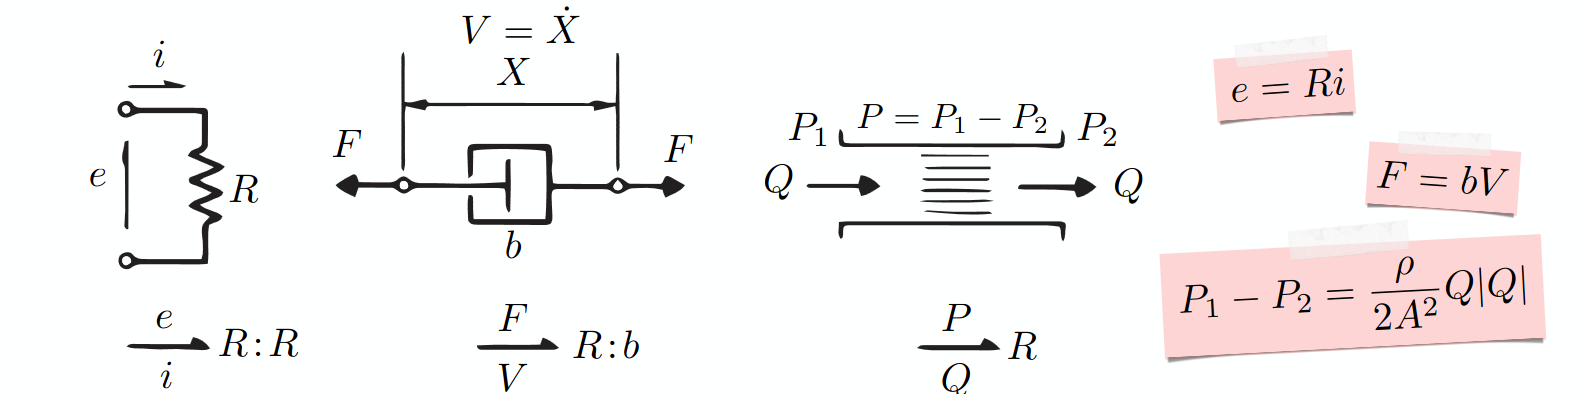
\includegraphics[scale=0.25]{figs/chapter2/2_1.png}
\caption{Different types of Resistive 1-port elements.}
\end{figure}

Physical realisations: electrical resistance $e=Ri$; viscous damper $F=bV$; fluid resistance $\Delta P = R_f Q$ (linear); orifice flow $\Delta P = k Q|Q|$ (nonlinear). 

In the bond graph:
\begin{center}
\begin{tikzpicture}[>=Stealth,every node/.style={font=\small}]
  \draw[thick,-stealth] (0,0) -- (1.2,0);
\node[draw,fill=gray!12,minimum width=1.0cm,minimum height=0.7cm,font=\small\bfseries]
    at (1.9,0) {R};
  \node at (-0.3,0.25) {$e$}; \node at (-0.3,-0.25) {$f$};
\node[font=\footnotesize,gray] at (5,0) {constitutive: $e=\mathcal{R}(f)$};
\end{tikzpicture}
\end{center}
The half-arrow points toward R (positive power convention). \textbf{For a linear element: appending \texttt{R:R} (or \texttt{R:b} for a damper) names the parameter}.


\begin{insightbox}[Causality of R]
The causality of a resistor is not fixed: it can be either effort-in or flow-in. This is because the constitutive relation is static, so if you impose one variable, the other is immediately determined without any integration or differentiation.
\end{insightbox}

\section{The 1-port capacitor \textit{C}: potential energy storage}

A capacitor (or compliance) stores \textbf{potential energy} via a static relationship between effort and displacement:
\begin{equation}
  e = \mathcal{C}^{-1}(q), \qquad q = \int f\,dt.
\end{equation}
In the linear case, $e = q/C$. The linear compliance $C$ is defined as the inverse of the slope of the $e$ versus $q$ constitutive curve.

Stored energy:
\begin{equation}
  E(q) = \int_{q_0}^q e(\bar{q})\,d\bar{q} \quad\longrightarrow\quad E = \frac{q^2}{2C} \text{ (linear)}.
\end{equation}

Usually $E_0$ is set to zero by offsetting the energy reference point.

Since the capacitor stores energy without loss, the power flow into the port can reverse, meaning power flows back out into the system. During this process, energy is strictly conserved.

\begin{figure} [H]
  \centering
  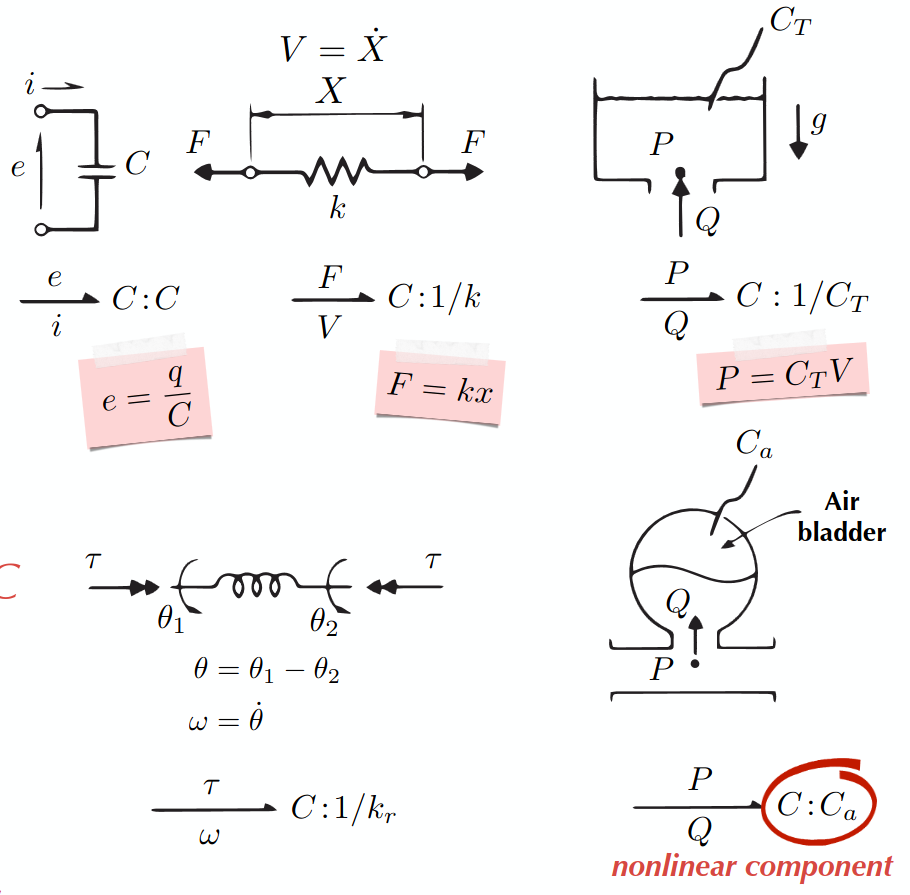
\includegraphics[scale=0.25]{figs/chapter2/2_2.png}
  \caption{Different types of Capacitive 1-port elements.}  
\end{figure}

Physical realisations: electrical capacitor $e = q/C$; spring $F = kx$ (so $C = 1/k$); hydraulic accumulator $P = V/C_a$; torsional spring $\tau = k_r\theta$.

\begin{insightbox}[Preferred causality of C]
A capacitor can either be in \textbf{integral causality} and in \textbf{derivative causality}.

$$
  e = \mathcal{C}^{-1}\biggl(\int f\,dt\biggr), \qquad f = \frac{d}{dt} \mathcal{C}(e).
$$

The natural causality for a capacitor is \textbf{flow-in, effort-out}: flow is integrated to give displacement, from which effort is computed. This is called \emph{integral causality}. If the bond graph forces effort-in on C (derivative causality), the element does not contribute an independent state variable, which has implications for the system's order.

Intuitively, from a simulation perspective, you impose the flow (e.g., current or velocity) which the element integrates into displacement (charge or position), and this displacement yields the effort (voltage or force) as an output.
\end{insightbox}

\section{The 1-port inertia \textit{I}: kinetic energy storage}

An inertia (inductor) stores \textbf{kinetic energy} via a static relationship between flow and momentum:
\begin{equation}
  f = \mathcal{I}^{-1}(p), \qquad p = \int e\,dt.
\end{equation}
In the linear case, $f = p/I$. Here, the linear inertia $I$ is defined as the inverse of the slope of the $f$ versus $p$ curve.

Stored energy:
\begin{equation}
  E(p) = \int_{p_0}^p f(\bar{p})\,d\bar{p} \quad\longrightarrow\quad E = \frac{p^2}{2I} \text{ (linear)}.
\end{equation}

Similarly to the capacitor, the $E_0$ reference point is typically set to zero.

\begin{figure} [H]
  \centering
  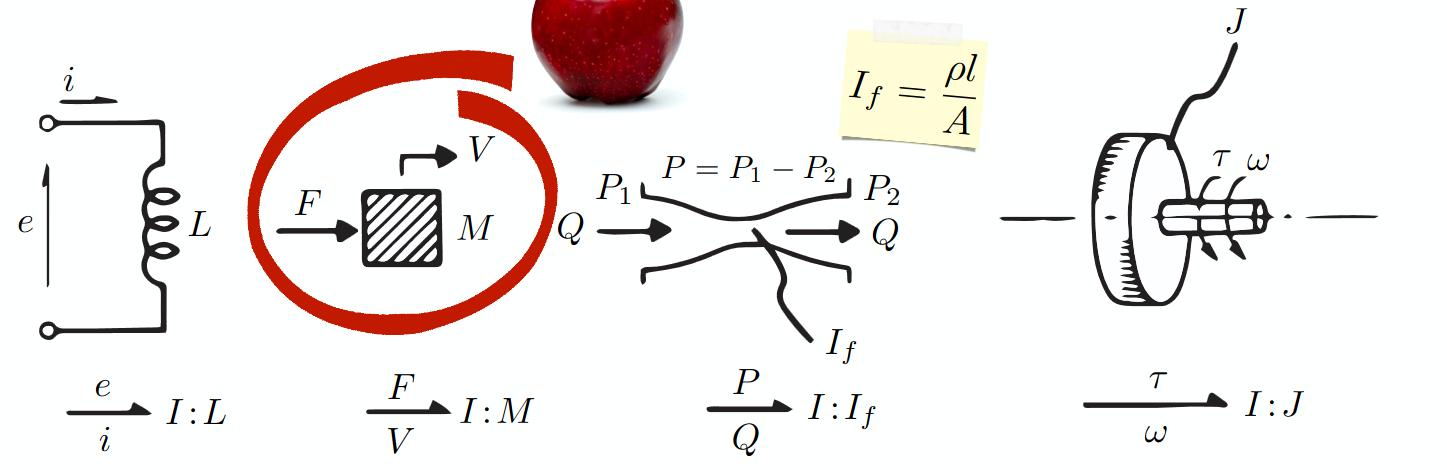
\includegraphics[scale=0.25]{figs/chapter2/2_3.png}
  \caption{Different types of Inertial 1-port elements.}
\end{figure}

Physical realisations: point mass $F = ma \Rightarrow V = P/m$ (so $I = m$); rotating body $\tau = J\dot{\omega} \Rightarrow \omega = p_\tau/J$; fluid inertance $\Delta P = I_f \dot{Q}$.

\begin{insightbox}[Preferred causality of I]
An inertia integrates force to give momentum, which means that it accumulates the effect of effort over time. The formula is $v = p/I$, so the flow (velocity) is derived from the momentum, which is $p = \int e\,dt$. If it was otherwise, and you imposed the flow (velocity), it would mean that imposing an abrupt change in velocity would require an infinite force, which is not physically realizable. 

\begin{equation}
  f = \mathcal{I}^{-1}\biggl(\int e\,dt\biggr), \qquad e = \frac{d}{dt} \mathcal{I}(f).
\end{equation}

The natural causality for an inertia is \textbf{effort-in, flow-out}: effort is integrated to give momentum, from which flow is computed. Again, this is integral causality. Newton's second law is a direct statement of this: force (effort) integrates to momentum, from which velocity (flow) is recovered. 

As with the capacitor, imposing flow on an inertia leads to derivative causality because the imposed flow must be differentiated to find the required effort, thus reducing the number of independent state variables (you lose position, hence memory).
\end{insightbox}

The tetrahedron of state variables  summarises the four types and their relationships: $\dot{p}=e$, $\dot{q}=f$, with C linking $e$--$q$ and I linking $f$--$p$.

\begin{figure} [H]
  \centering
  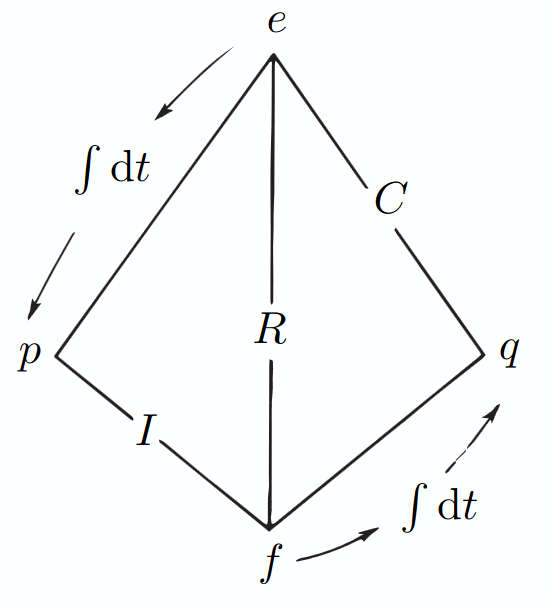
\includegraphics[scale=0.25]{figs/chapter2/2_4.png}
  \caption{Tetrahedron of state variables.}
\end{figure}

\section{Source elements \textit{Se} and \textit{Sf}}

An \textbf{effort source} $Se$ maintains a specified effort $e(t)$ at its port, regardless of the flow (infinite power if needed, the idealisation of a stiff voltage/force/pressure supply). A \textbf{flow source} $Sf$ dually maintains a specified flow. 

\textbf{Their causality is fixed}: $Se$ always imposes effort (causal stroke away from $Se$); $Sf$ always imposes flow.

\begin{figure} [H]
  \centering
  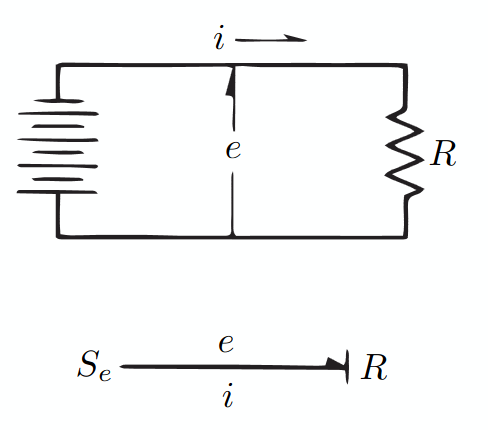
\includegraphics[scale=0.25]{figs/chapter2/2_5.png}
  \caption{Example of source elemets. Voltage generator and resistor in series, with $Se$ imposing voltage and $R$ determining current.}
\end{figure}

In reality, components always find a compromise. For instance, when you set the voltage of a real battery, the act of drawing current inherently lowers the voltage itself. Because ideal sources do not model this compromise in one go, a real-world component like a battery must be modeled using an ideal voltage source ($Se$) in series with a resistance ($R$) to accurately simulate the voltage drop under load.

When the source value is itself a function of a signal from another part of the graph, it becomes a \textbf{modulated source} MSe or MSf. This is how controlled actuators, variable-flow pumps, and vibration shakers are represented.

\begin{figure} [H]
  \centering
  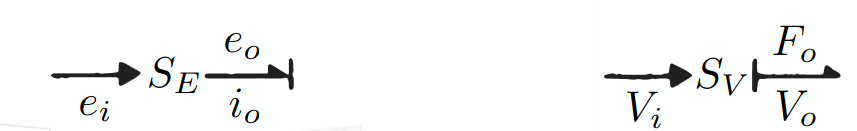
\includegraphics[scale=0.25]{figs/chapter2/2_6.png}
  \caption{Modulated source of effort (MSe) and modulated source of flow (MSf).}
\end{figure}

\section{The transformer \textit{TF}: effort--effort, flow--flow exchange}

A transformer is a \textbf{power-conserving 2-port}: $e_1 f_1 = e_2 f_2$ at all times. Its constitutive relations scale effort and flow by a constant (or time-varying) modulus $m$:
\begin{equation}
  \begin{cases}
    e_1 = m \, e_2 \\
    m \, f_1 = f_2
  \end{cases}
\end{equation}
Effort is scaled up by $m$, flow is scaled down by $m$ (or vice versa).

\begin{figure}[H]
  \centering
  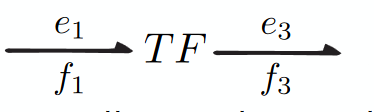
\includegraphics[scale=0.25]{figs/chapter2/2_7.png}
  \caption{Bond graph symbol for the transformer element.}
\end{figure}


Physical examples: electrical transformer ($m = N_1/N_2$, turns ratio); lever ($m = b/a$, arm ratio); hydraulic piston ($F = AP$, $AV = Q$, so $m = A$); gear pair ($m = r_1/r_2$); rack and pinion.

\begin{figure}[H]
  \centering
  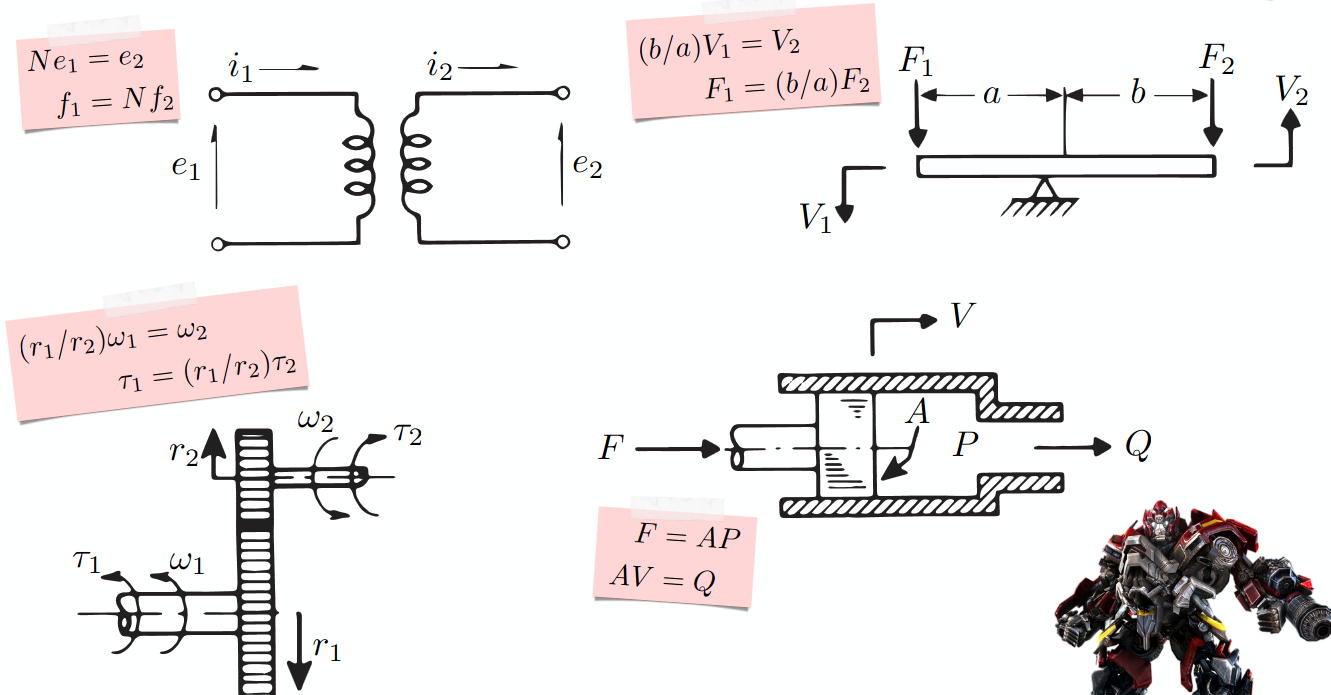
\includegraphics[scale=0.25]{figs/chapter2/2_8.png}
  \caption{Physical examples of transformer elements.}
\end{figure}


\begin{insightbox}[TF causality]
Two causal forms are valid for TF: either effort-in on port 1 (and effort-out on port 2), or effort-in on port 2. The causal stroke must appear on exactly one of the two ports. 

\end{insightbox}

If the geometry changes (e.g.\ a linkage), $m$ becomes time-dependent, the element becomes a \textbf{modulated transformer} MTF. 
\begin{figure} [H]
  \centering
  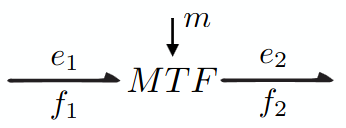
\includegraphics[scale=0.25]{figs/chapter2/2_14.png}
  \caption{Modulated transformer (MTF).}
\end{figure}

In robotics, the Jacobian matrix plays the role of the MTF modulus. The Jacobian expresses the relationship between end-effector and joint velocities ($v = J(\theta)\dot{\theta}$). Assuming power conservation, it naturally also relates the end-effector applied force to the joint torques ($\tau = J^T(\theta)F$).

\section{The gyrator \textit{GY}: effort--flow exchange}

A gyrator is also power-conserving, but it exchanges the roles of effort and flow:
\begin{equation}
  e_1 = r\,f_2, \qquad r\,f_1 = e_2.
\end{equation}

\begin{figure} [H]
  \centering
  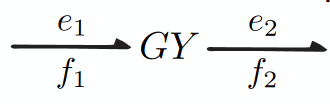
\includegraphics[scale=0.25]{figs/chapter2/2_9.png}
  \caption{Bond graph symbol for the gyrator element.}
\end{figure}

This is fundamentally different from TF: while a transformer maps effort to effort and flow to flow through a constant, the gyrator maps a flow to an effort and vice versa through a constant. 

\begin{figure}[H]
  \centering
  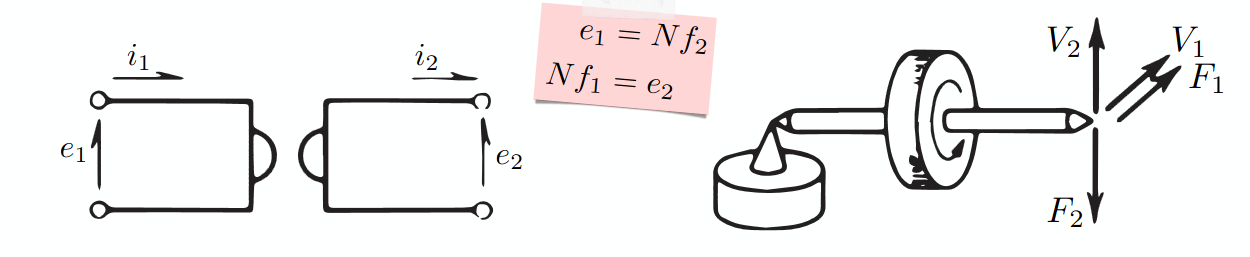
\includegraphics[scale=0.25]{figs/chapter2/2_10.png}
  \caption{Example of gyrator element.}
\end{figure}

\begin{figure}[H]
  \centering
  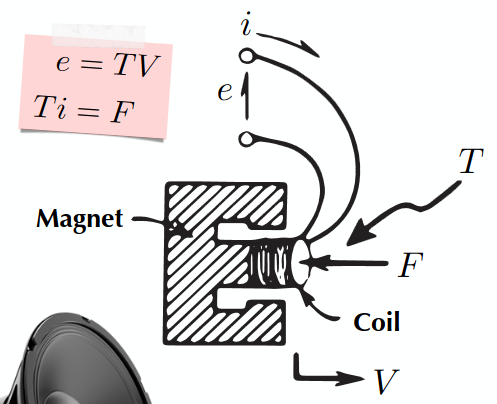
\includegraphics[scale=0.25]{figs/chapter2/2_11.png}
  \caption{More example of gyrator element.}
\end{figure}

Physical examples: DC motor (back-EMF $e_a = T\omega$, torque $Ti_a = \tau$, so $r = T$); gyroscope (a force in one direction induces an angular velocity in the perpendicular direction).

\begin{insightbox}[Gyrator is more fundamental than transformer]
The gyrator can sometimes seem like a mysterious element, but it is actually more fundamental than a transformer. Two cascaded gyrators produce a transformer. 

\begin{figure} [H]
  \centering
  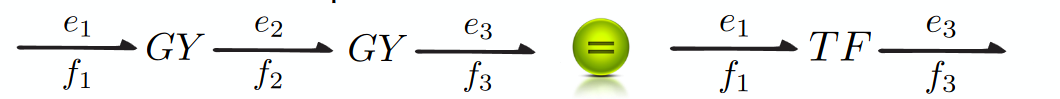
\includegraphics[scale=0.25]{figs/chapter2/2_12.png}
  \caption{Gyrator as a fundamental element.}
\end{figure}

More profoundly, a gyrator essentially interchanges the roles of effort and flow, so it maps C-elements into I-elements: a capacitor seen through a gyrator behaves as an inertia. This means one does not fundamentally need two types of energy-storage elements, the gyrator generates one from the other. Historically, ignoring gyrators and forcing gyroscopic systems into transformer notation led to incorrect models.

\begin{figure} [H]
  \centering
  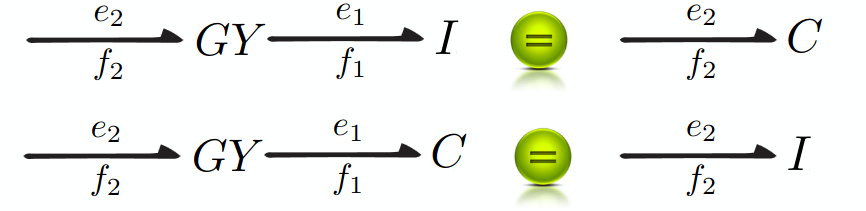
\includegraphics[scale=0.25]{figs/chapter2/2_13.png}
  \caption{Gyrator mapping C to I and vice versa.}
\end{figure}

\end{insightbox}


When the gyration ratio $r$ depends on a signal (e.g.\ motor torque constant varying with field current), the element becomes a modulated gyrator \textbf{MGY}.

\begin{figure} [H]
  \centering
  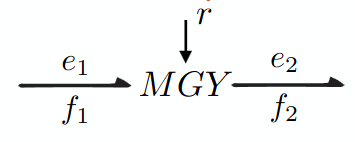
\includegraphics[scale=0.3]{figs/chapter2/2_15.png}
  \caption{Modulated gyrator (MGY).}
\end{figure}

\section{Junction elements: 0-junction and 1-junction}

Junctions are \textbf{power-conserving} multi-port elements that distribute power among connected elements. They enforce algebraic constraints on efforts and flows. Fundamentally, zero and one junctions are simply mathematical \textbf{conditions} applied to the system (such as force balance, flow conservation, or parallel branches sharing the same voltage).

\subsection{The 0-junction: common effort}

At a 0-junction all connected bonds share the \textbf{same effort}, and the flows sum algebraically to zero (with signs set by the half-arrow directions):
\begin{equation}
  e_1 = e_2 = e_3 = \cdots, \qquad \sum_k \pm f_k = 0.
\end{equation}

\begin{figure}[H]
  \centering
  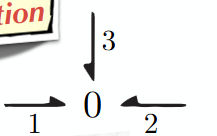
\includegraphics[scale=0.4]{figs/chapter2/2_16.png}
  \caption{Bond graph symbol for the 0-junction element.}
\end{figure}

Electrical analogue: a \textbf{node} (Kirchhoff's current law, same voltage). Mechanical analogue: a point where a single force acts on several elements with velocities that sum to zero (geometric compatibility, spring and damper in parallel). Here, we are imposing a relation between relative velocities. Hydraulic analogue: a junction of pipes (conservation of volume flow).

\subsection{The 1-junction: common flow}

At a 1-junction all connected bonds share the \textbf{same flow}, and the efforts sum algebraically to zero:
\begin{equation}
  f_1 = f_2 = f_3 = \cdots, \qquad \sum_k \pm e_k = 0.
\end{equation}

\begin{figure} [H]
  \centering
  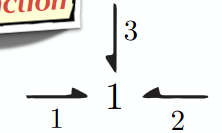
\includegraphics[scale=0.4]{figs/chapter2/2_17.png}
  \caption{Bond graph symbol for the 1-junction element.}
\end{figure}

Electrical analogue: a \textbf{loop} (Kirchhoff's voltage law, same current). Mechanical analogue: Newton's law for a mass, all forces acting on an inertia sharing a single velocity must balance. It encodes the action-reaction principle and effectively acts as a rigid connection among the mechanical elements. Hydraulic analogue: pressure drops around a single-flow circuit sum to zero.



\begin{warningbox}[Sign conventions at junctions]
The algebraic sum at a junction depends on the \emph{direction of the half-arrows}. One convention: at a 0-junction, the half-arrow of the ``driving'' bond points \emph{toward} the junction, and all others point away, then the sum of all $f_k$ equals the driving flow
\end{warningbox}

\subsection{Bond graph identities and simplification}

A 0-junction with only two bonds connecting to it reduces to direct connection (same effort, same flow). A 1-junction with only two bonds similarly reduces. These \textbf{bond graph identities} allow systematic simplification of an initial, verbose bond graph into a compact one. They are used heavily when eliminating zero-power bonds (e.g.\ after connecting to ground in a mechanical model) and when simplifying ``reducible loops'' that appear when spring and damper share the same relative velocity.

For \textbf{generalizing n-port components} there exist specific rules. 

\begin{figure} [H]
  \centering
  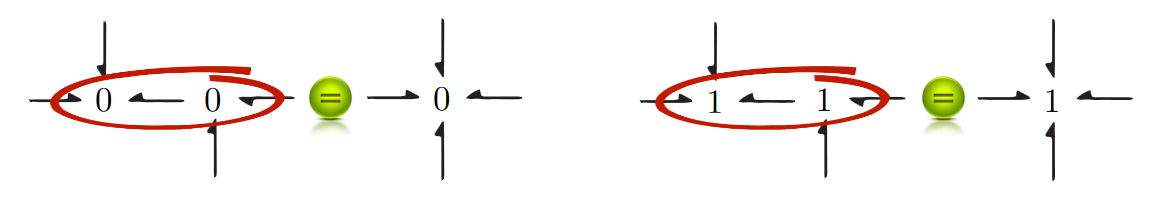
\includegraphics[scale=0.25]{figs/chapter2/2_18.png}
  \caption{Rules for simplifying n-port elements}
\end{figure}

\section{Causality summary for basic elements}

For effort and flow sources, causality is trivial and fixed. For basic 2-ports (TF, GY), there are two possible causal assignments; as soon as one variable is assigned as an input, the other is constrained by the constitutive relation. Similar logic naturally extends to 3-ports (junctions).


\begin{center}
\begin{tabular}{llll}
  \toprule
  \textbf{Element} & \textbf{Preferred causality} & \textbf{Alternative} & \textbf{Notes}\\
  \midrule
  Se & effort out (fixed) & - & always imposes $e$\\
  Sf & flow out (fixed) & - & always imposes $f$\\
  R  & either & either & indifferent (usually)\\
  C  & flow in (integral) & effort in (derivative) & derivative $\Rightarrow$ dependent state\\
  I  & effort in (integral) & flow in (derivative) & derivative $\Rightarrow$ dependent state\\
  TF & one of two forms & - & must be one in, one out\\
 
  GY & both in \emph{or} both out & - & two valid forms\\
  0-jct & one effort in, rest out & - & uniquely determined\\
  1-jct & one flow in, rest out & - & uniquely determined\\
  \bottomrule
\end{tabular}
\end{center}


Causality and bond graphs are very important. Indeed it's possible to predict many important features of the system
even before the constituitve laws for all the elements have been specified. 

It's possible to predict the number of state variables and it's useful for writing state equations. 

\vspace{0.5cm}


Once the causal stroke is added, it's possible to transform the bond graph into a block diagram.
They are more complex since a single bond represent two signal flows.
 %%%%%%%%%%%%%%%%%%%%%%%%%%%%%%%%%%%%%%%%%%%%%%%%%%%%%%%%%%%%%%%%%%%%%%%
\chapter{System Models in Different Domains}
\label{ch:systemmodels}
%%%%%%%%%%%%%%%%%%%%%%%%%%%%%%%%%%%%%%%%%%%%%%%%%%%%%%%%%%%%%%%%%%%%%%%


\section{Electrical circuits and networks}

Any electrical circuit can be modelled by a bond graph containing elements of the set $\{ 0, 1, R, C, I, Se, Sf \}$. For electrical circuits the mapping to bond graph variables is direct: voltage is effort, current is flow. The 0-junction encodes Kirchhoff's current law at a node (same voltage, currents sum to zero); the 1-junction encodes Kirchhoff's voltage law around a loop (same current, voltage drops sum to zero).

$TF$ and $GY$ are not included since they are used to represent electrical networks.

\begin{itemize}
  \item 0 Junction: Same voltage
  \item 1 Junction: Same current
\end{itemize}


\paragraph{Construction procedure.}
Constructing the overall bond graph model is much easier if a procedure can be followed that ensures success regardless of the complexity.

\begin{figure} [H]
\centering 
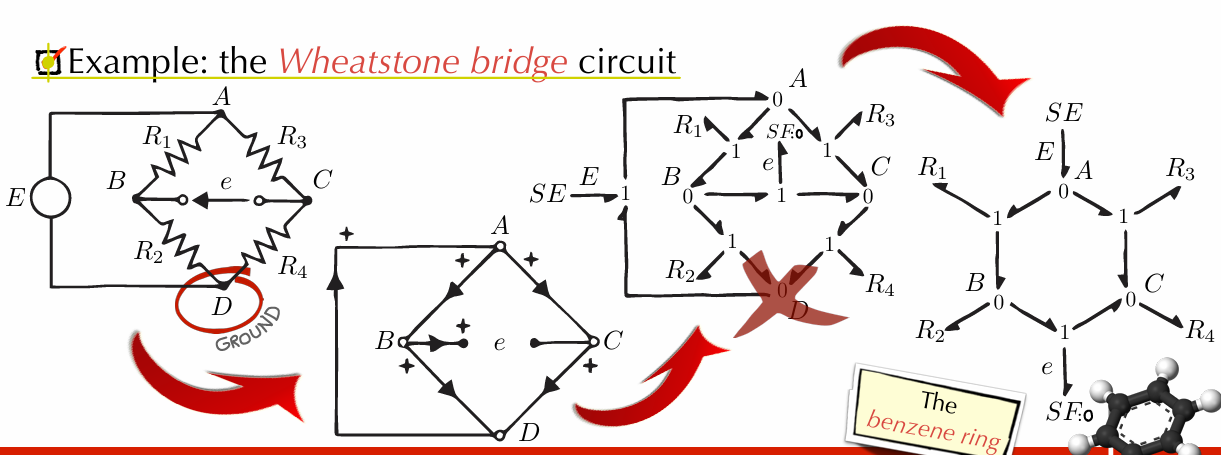
\includegraphics[scale=0.25]{figs/chapter3/3_1.png}
\caption{Example of electric circuit}
\end{figure}

\begin{enumerate}[leftmargin=2em,itemsep=2pt]
  \item \textbf{Assign a power convention}: for each circuit element choose positive current direction and positive voltage drop. Talking about power in BG, we typically ensure that, when positive, power is flowing \emph{towards} the passive 1-port element. Note that active elements are elements providing power (sources, but also energy-storing elements freeing their energy). In some situations, sources may even absorb power.
  \item \textbf{One 0-junction per node voltage}: place a 0-junction for every distinct node voltage (including what will be the ground). Every bond touching a 0-junction carries the same effort (node voltage).
  \item \textbf{One 1-junction per element}: for each circuit element (R, L, C, source), insert a 1-junction to represent the voltage difference across it. By properly directing the half-arrows on 1-junctions, the voltage drop can be established across each element. Connect the 1-junction between the two 0-junctions at its terminals. Attach the bond graph element (R, I, C, Se, Sf) to the 1-junction.
  \item \textbf{Ground = zero effort source}: choose a ground node and connect the ground 0-junction to a Sf~: 0 (zero-flow source) or Se~: 0 (zero-voltage), which in practice means deleting all bonds with zero power at that junction. Note that different bond graphs will result for a given circuit if we choose different ground nodes.7


  \begin{figure} [H]
  \centering
  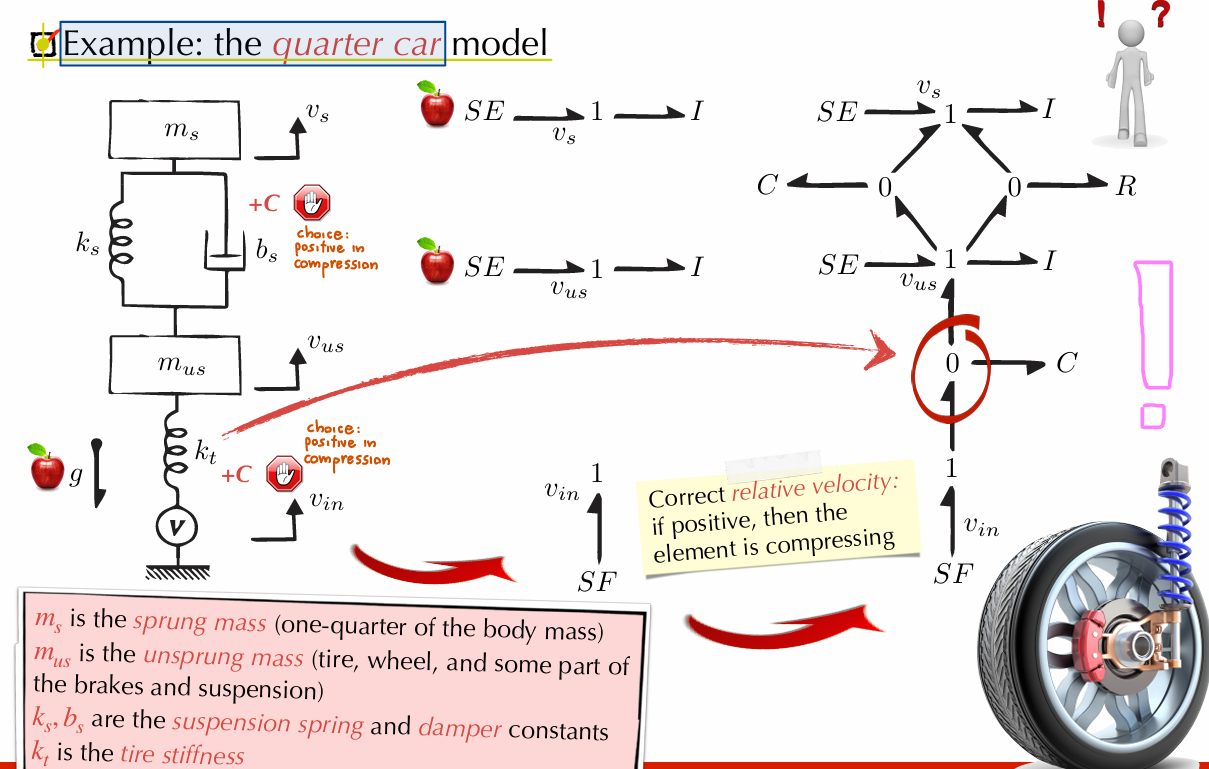
\includegraphics[scale=0.25]{figs/chapter3/3_2.png}
  \caption{Example of bond graph construction for the circuit in Fig. 3.1.}
  \end{figure}



  \item \textbf{Simplify}: apply bond graph identities to remove redundant junctions and bonds.
\end{enumerate}

\begin{figure} [H]
\centering
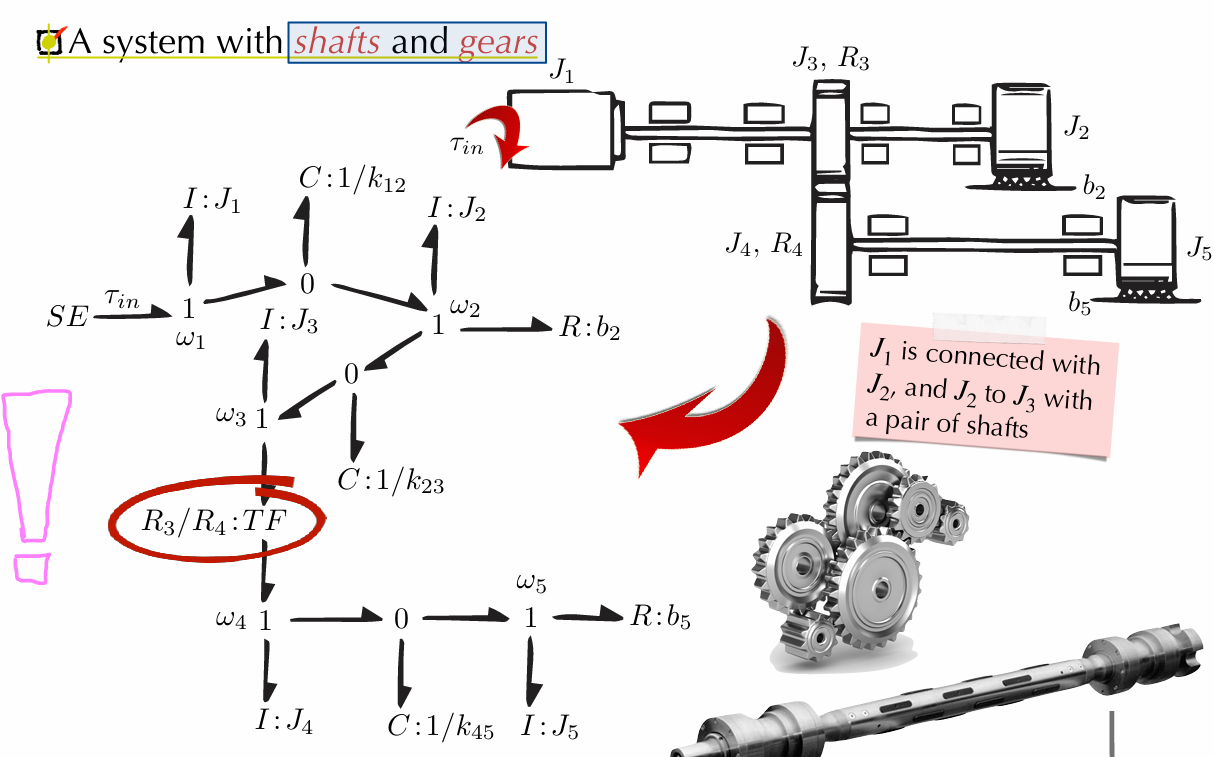
\includegraphics[scale=0.25]{figs/chapter3/3_3.png}
\caption{Example of bond graph simplification.}
\end{figure}


An electrical network is an extension of electrical circuits to include idealised transformers $TF$ and gyrators $GYG$. 



\subsubsection{Electrical Transformers}
It's used used to to step voltages up or down. 

\begin{figure} [H]
\centering
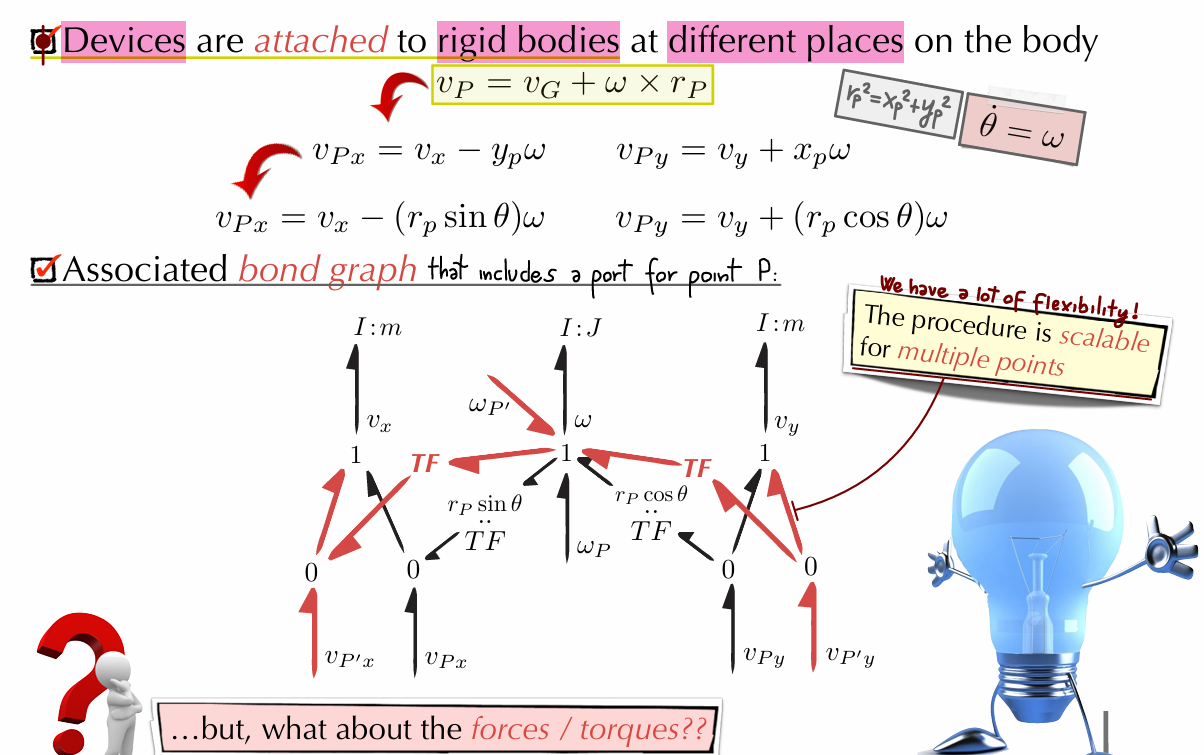
\includegraphics[scale=0.25]{figs/chapter3/3_4.png}
\caption{Ideal transformer with turns ratio $N$.}
\end{figure}


\subsubsection{Electrical Gyrators}

Electrical gyrators are exhibited in Hall effect transducers, where voltage across a semiconductor material is related to a current through the material perpendicular to the voltage drop direction. The same construction method extends to \textbf{electrical networks} containing transformers (TF) and gyrators (GY). The transformer element inserts between two 1-junctions; the turns ratio $N$ becomes the TF modulus. The basic rules for bond graph construction remain unchanged.



\begin{insightbox}[Ladder and T/pi structures]

\begin{figure} [H]
\centering
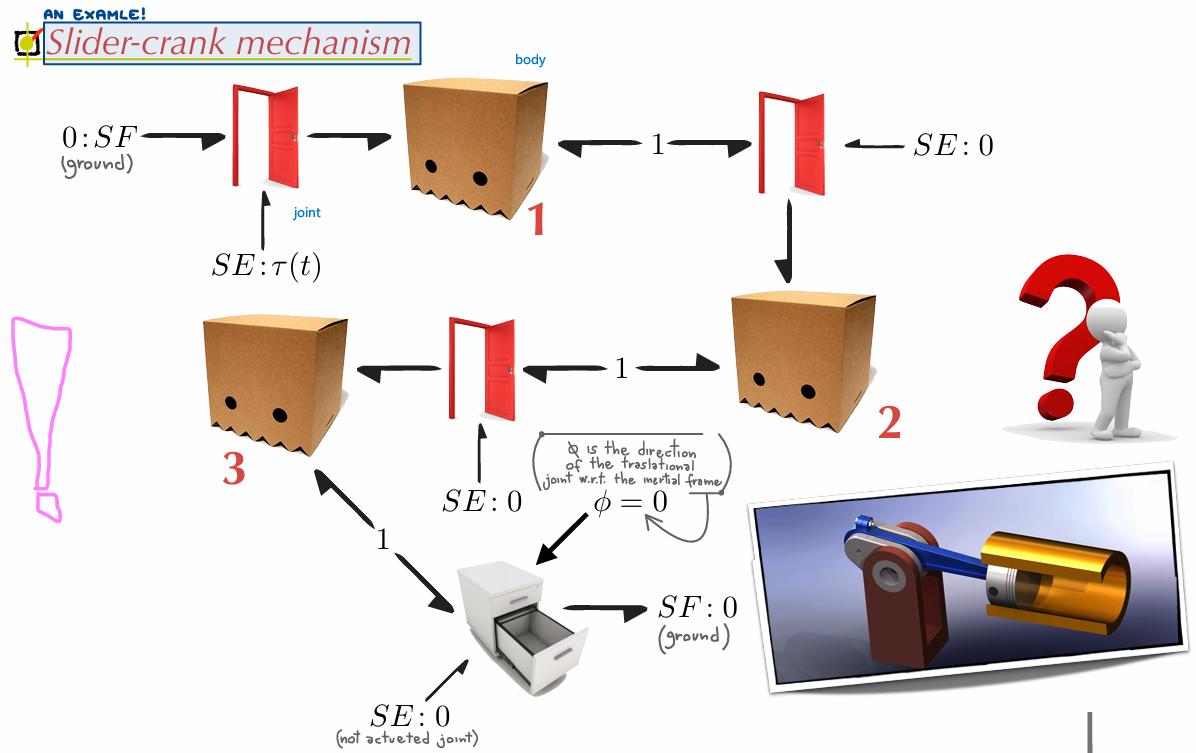
\includegraphics[scale=0.25]{figs/chapter3/3_5.png}
\caption{Resistive ladder with resistors}
\end{figure}

Transmission lines and long hydraulic lines have lumped approximations as ladder networks  cascaded T or pi sections. 
In bond graph terms, the T-section corresponds to alternating 1-junctions (series inductors) and 0-junctions (shunt capacitors). 
The topological dual (exchanging 0 and 1 junctions) gives the pi-section. Notice that the difference between these two schemes is the role of current and voltage is interchanged. This technique holds in general when we want to find the topological dual of even complex circuits: exchange 0 and 1 junctions in the BG!
The pi and tee structures become truncations of the ladder structure that allow for reasonable inclusion of some of the \textbf{transmission line dynamics without having the overall system become too large}. Understanding this duality is a powerful shortcut when building bond graphs by inspection.

\begin{figure} [H]
\centering
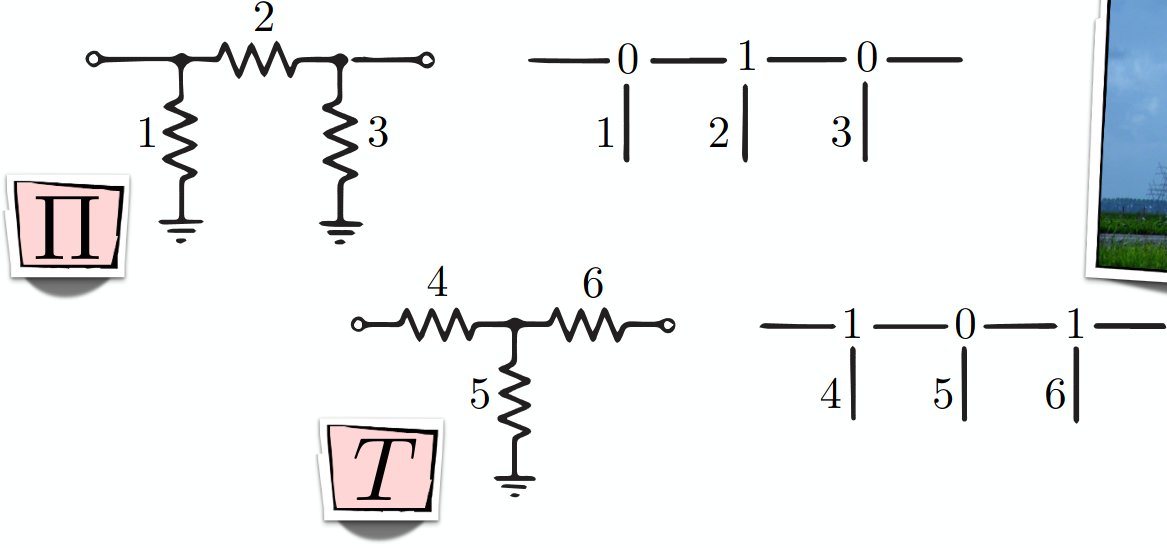
\includegraphics[scale=0.25]{figs/chapter3/3_6.png}
\caption{pi and tee sections as truncations of the ladder structure.}
\end{figure}


\end{insightbox}

\section{Mechanical translation}

Mechanical systems are those composed of components such as masses, springs, dampers, levers, flywheels, gears, shafts, and so forth. When dynamic systems are put together from these components, we must interconnect rotating and translating inertial elements with axial and rotational springs and dampers, and we must appropriately account for the kinematics of the systems.

For mechanical translation, velocity is flow and force is effort. The analogy with electrical circuits is \emph{dual}: in electrical circuits, nodes share voltage (0-junction); in mechanics, rigid connections share velocity (1-junction). 

\begin{itemize}
  \item 0 Junction: Relative velocity (force-generating elements)
  \item 1 Junction: Same velocity
\end{itemize}

\paragraph{Construction procedure for Mechanical Translation.}
\begin{enumerate}[leftmargin=2em,itemsep=2pt]
  \begin{figure} [H]
    \centering
    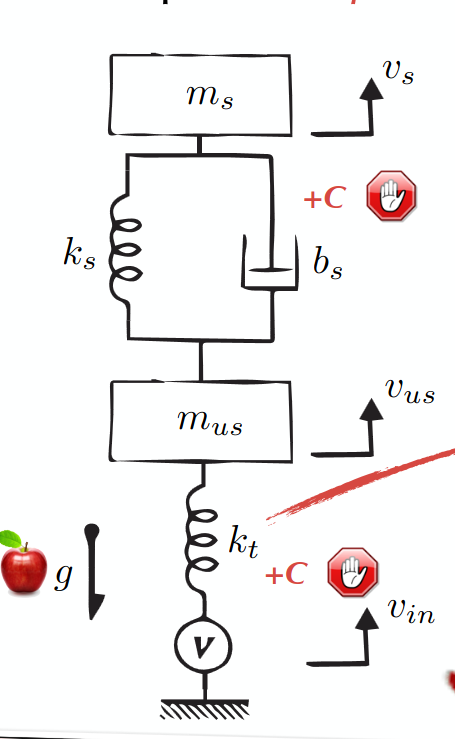
\includegraphics[scale=0.25]{figs/chapter3/3_7.png}
    \caption{Example of mechanical system with translation.}
  \end{figure}

  \item \textbf{Indicate velocity directions}: on a free-body-type sketch, use arrows and symbols to indicate the positive direction of absolute velocity components. Fixing conventional directions in this scheme is the first crucial step! State whether force-generating elements are positive in tension or compression using symbols such as +T or +C.
  \begin{figure} [H]
  \centering
  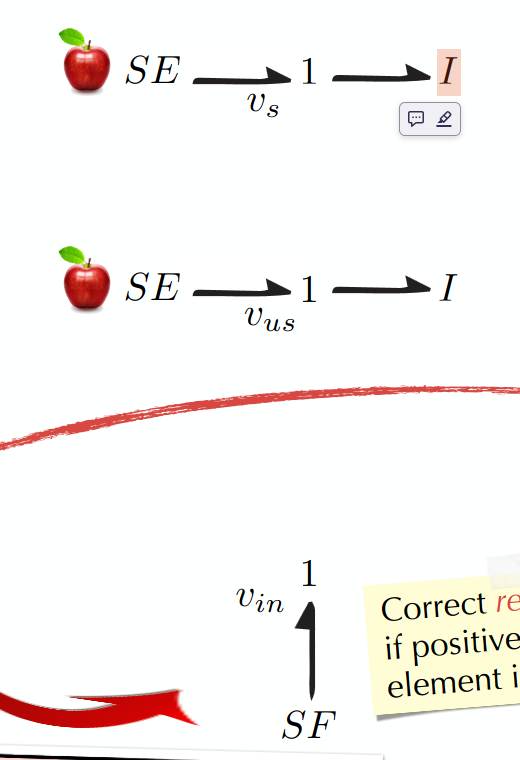
\includegraphics[scale=0.25]{figs/chapter3/3_8.png}
  \caption{Example of free-body sketch with velocity directions and force conventions.}
  \end{figure}

  \item \textbf{One 1-junction per distinct velocity}: each inertia is attached to its absolute velocity 1-junction.
  \item \textbf{0-junctions for relative velocities}: spring and damper forces react to the rate of extension, meaning they depend on the \emph{relative} velocity across them. A 0-junction connecting two 1-junctions produces the relative velocity difference needed by the compliant/resistive element. The sign at the 0-junction must be chosen so that the relative velocity is positive when the element is in the assumed tension/compression state. When forces are positive in tension, power will flow toward the elements.
  

  \begin{figure}[H]
  \centering
  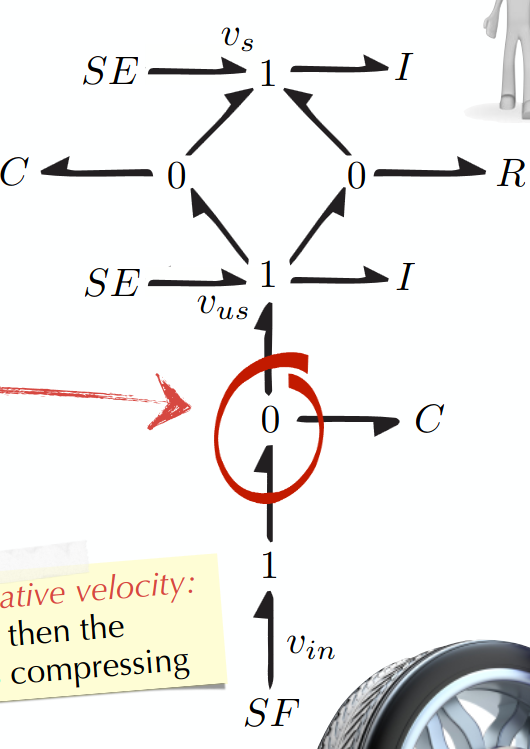
\includegraphics[scale=0.25]{figs/chapter3/3_9.png}
  \caption{Example of bond graph construction for the mechanical system in Fig. 3.7.}
  \end{figure}


  \item \textbf{Reference (ground)}: the inertial frame is fixed in zero velocity, represented by a Sf~: 0, which is deleted after establishing relative velocities.
  \item \textbf{Attach elements}: inertias on 1-junctions; springs (C~: $1/k$) and dampers (R~: $b$) on their relative-velocity 0-junctions; gravity and other absolute forces as Se sources on velocity 1-junctions.
\end{enumerate}

The \emph{beauty} of power conservation in junctions is that we need only to constrain the velocities, and the forces will be automatically balanced without further effort. Newton's second law and the action-reaction principle are built in without explicitly writing them. We can perform a double check to see that the force balance is realized by the 1-junctions.



\paragraph{Reducible loop.}
When a spring and damper are in parallel (same relative velocity), the 0-junction connecting both their velocity 1-junctions can be simplified using bond graph identities into a single 0-junction carrying both the C and R elements. This is the \textbf{reducible loop} , a very common pattern that emphasizes that several elements share exactly the same relative velocity.

\paragraph{Levers, pulleys and kinematic linkages.}
With minor efforts, it is possible to deal with translational systems containing levers, pulleys, and other simple motion-force transforming devices. These introduce position-dependent force/velocity transformations, represented by modulated transformers (MTF) or fixed TF when the geometry is constant. The MTF modulus is the relevant geometric ratio (e.g.\ the Jacobian in robotics).

\section{Fixed-axis rotation}

Fixed-axis rotation occurs in the mechanics of rotating machines, such as electric motors and internal combustion engines, gear boxes, transmissions, transfer cases, differentials, and drive shafts.

Only minor modifications to the procedure for mechanical translation allow handling systems with fixed-axis rotation. It is entirely analogous to translation with the variable substitution $V \to \omega$, $F \to \tau$, $m \to J$, $k \to k_r$, $b \to b_r$. 

The construction procedure is identical: 1-junctions for distinct absolute angular velocities, 0-junctions for relative angular velocity across compliant or resistive rotational elements, TF for gear pairs (modulus = gear ratio $r_1/r_2$), and eliminating the bonds with zero angular velocity.

In the fixed-axis rotation framework, it's not really relevant to talk about +T or +C; what is relevant is to maintain coherence with the relative velocities across all the schemes (e.g., choosing one velocity as the upstream master velocity and the other as the downstream slave velocity).

\begin{figure} [H]
\centering
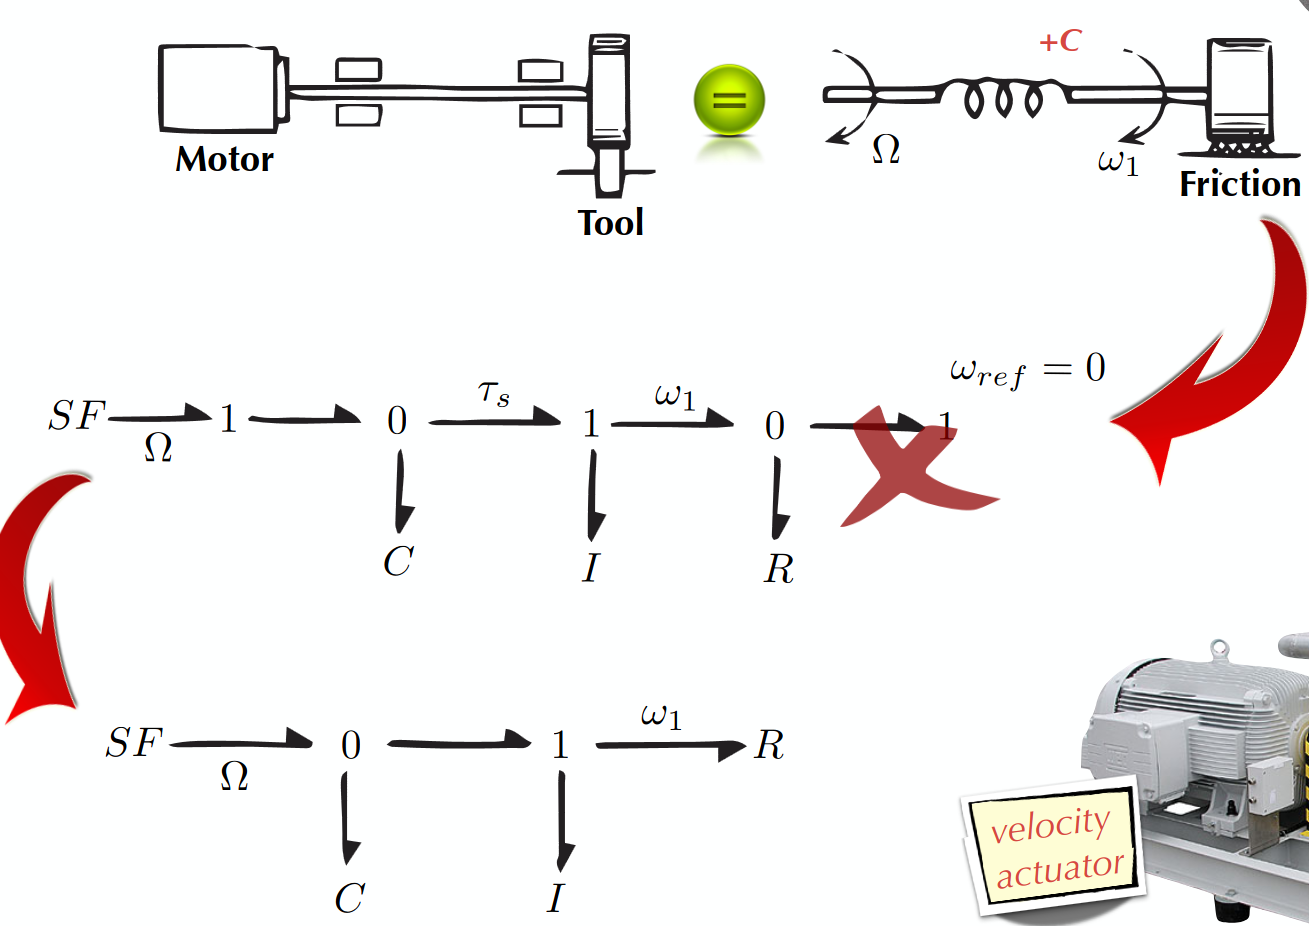
\includegraphics[scale=0.25]{figs/chapter3/3_10.png}
\caption{Example of bond graph construction for a fixed-axis rotational system.}
\end{figure}


\section{Plane motion of rigid bodies}

Mechanical bodies with finite mass both translate and rotate in real applications; their dynamics are governed by a simultaneous combination of translation and rotation. 3-D motion is not trivial, so plane motion is much simpler. Plane motion results when the inertial bodies of a physical system are constrained to translate in two dimensions and to rotate only about an axis perpendicular to the plane of motion. The motion is always w.r.t. an inertial frame (with eventually coordinate transformations in the middle).

When a body both translates and rotates in a plane, three absolute velocity components are needed: $v_x$, $v_y$ (translational velocities of the centre of mass) and $\omega$ (angular velocity). Newton's law in the plane gives three 1-junctions, one per component, each with its own inertia element:

\begin{equation}
  m\dot{v}_x = F_x, \quad m\dot{v}_y = F_y, \quad J\dot{\omega} = \tau,
\end{equation}

\begin{figure} [H]
\centering
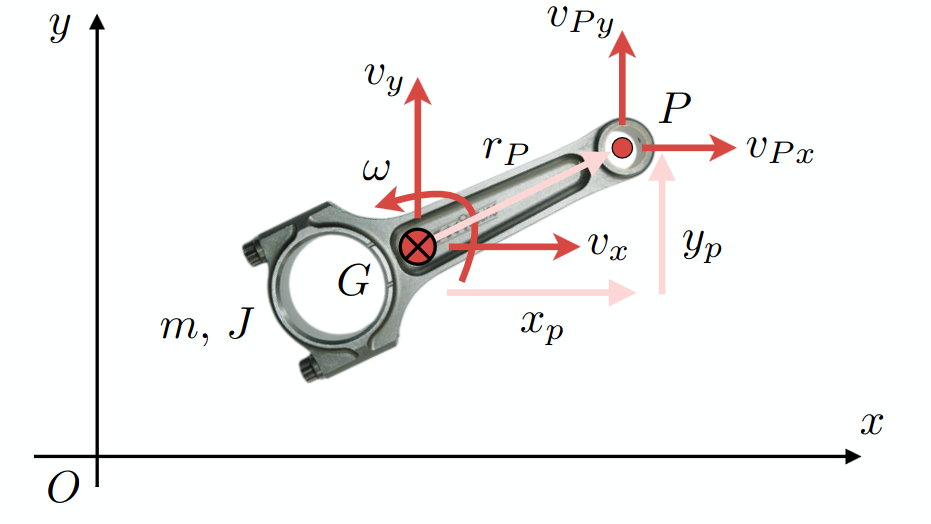
\includegraphics[scale=0.25]{figs/chapter3/3_11.png}
\caption{Mechanical body}
\end{figure}

\begin{figure} [H]
  \centering
  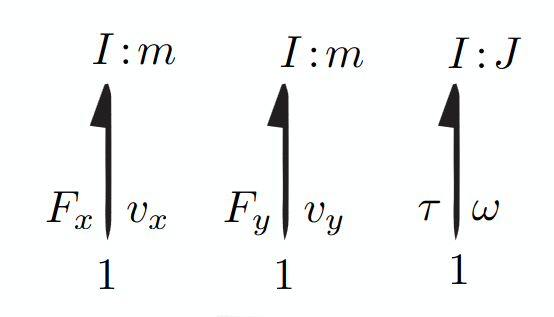
\includegraphics[scale=0.25]{figs/chapter3/3_12.png}
  \caption{Bond graph representation of the plane motion of a rigid body.}

\end{figure}

so the kinetic energy is $T = \frac{1}{2}m v_x^2 + \frac{1}{2}m v_y^2 + \frac{1}{2}J\omega^2$ with three I-elements. This dynamic representation does not involve directly any position information, which is coherent with the fact that this object stores kinetic energy, not potential energy.

Devices are attached at points $P$ offset from the centre of mass by $(r_P\cos\theta, r_P\sin\theta)$ in the inertial frame. The velocity of point $P$ is:
\begin{equation}
  v_{Px} = v_x - (r_P\sin\theta)\omega, \qquad
  v_{Py} = v_y + (r_P\cos\theta)\omega.
\end{equation}
These are linear combinations of the three body-velocity components, implemented with MTF elements (moduli $r_P\sin\theta$ and $r_P\cos\theta$, time-varying through $\theta$). By power conservation ($\Delta F_x v_x + F_y v_y + \tau \omega = F_{Px}v_{Px} + F_{Py}v_{Py} + \tau_P \omega_P$), the corresponding forces and torques at the body's ports are automatically balanced without writing free-body equations explicitly. The result is an "object" with a force/velocity interface toward the environment (what is outside the system). All the port variables are expressed with respect to the inertial frame. 


\begin{insightbox}[Parenthesis: the Body Frame!]
To characterize the energy of a rigid body, it is necessary to know the velocity of the center of mass and the angular velocity. The velocities discussed so far are expressed in the inertial reference, but for multi-body dynamics, it is sometimes convenient to introduce body-fixed coordinates. This coordinate frame remains attached to the center of mass and moves with the body. The advantage is that the inertial tensor is constant, unlike in the inertial frame where it varies with the configuration of the mechanism. 
However, expressing absolute accelerations in the body frame requires additional terms (e.g., $a_x = \dot{v}_X - \omega v_Y$). While body frames are generally preferred to have a constant inertial tensor, in the planar case, inertial frames can be used without any problems.

We can see the body dynamics as a "black box" with three ports (two for translation and one for rotation) that can be connected to the environment. The internal structure of the body is not relevant for the external behavior, which is fully characterized by the kinetic energy and the force/velocity relations at the ports. This is a powerful abstraction that allows us to model complex systems without needing to know all the internal details of each component.

\begin{figure} [H]
  \centering
  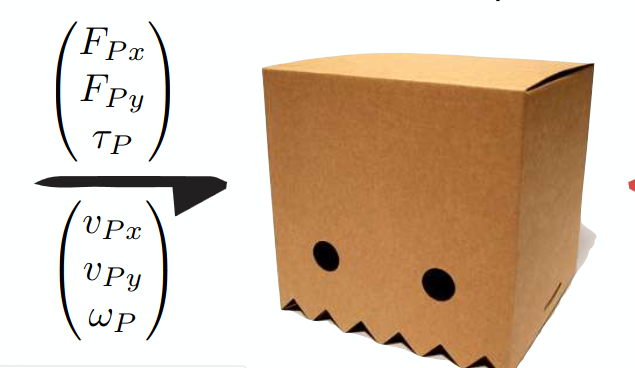
\includegraphics[scale=0.25]{figs/chapter3/3_13.png}
  \caption{Black-box representation of a rigid body with three ports.}
\end{figure}

\end{insightbox}

\paragraph{Connecting rigid bodies: joints.}
Going back to the formulation in the inertial frame, to interconnect rigid bodies and obtain complex mechanisms, it is necessary to define joints that constrain motion in specific directions.
A \textbf{rotational joint} constrains the two connected bodies to have the same position (zero relative linear velocity) while leaving angular velocity free. Any difference in angular velocity ($\omega_r = \omega_B - \omega_A$) means a torque exists.

\begin{figure} [H]
\centering
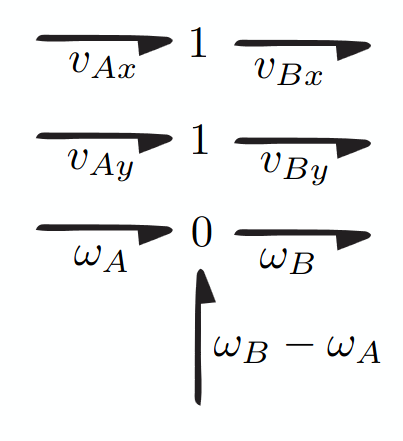
\includegraphics[scale=0.25]{figs/chapter3/3_14.png}
\caption{Rotational joint connecting two bodies.}
\end{figure}


A \textbf{translational joint} constrains relative motion to one direction. Since velocities are in the inertial frame, this direction is not fixed and is related to an angle $\phi$. The relative velocities must be transformed into the direction of the joint.
Both are represented by setting appropriate velocity-difference bonds to zero and using MTF elements for the direction transformation in the inertial frame. This is the basis for the bond graph modelling of robot manipulators and mechanisms.


\begin{figure} [H]
\centering
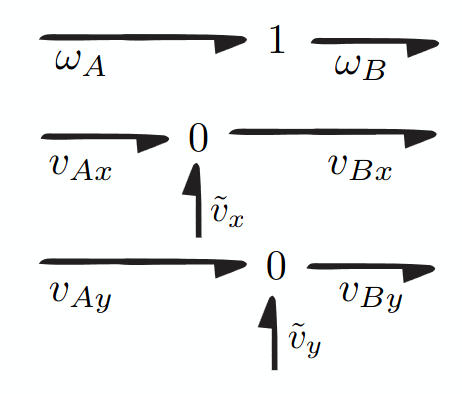
\includegraphics[scale=0.25]{figs/chapter3/3_15.png}
\caption{Translational joint connecting two bodies.}
\end{figure}

\begin{figure}[H]
\centering
% \includegraphics[scale=0.25]{figs/chapter3/3_16.png}
\caption{Rotation of the relative velocity. Instead of dividing by $cos$ and $sin$, we use a trick with a MTF}
\end{figure}


\section{Hydraulic and acoustic circuits}

\begin{itemize}
  \item One category is \textbf{hydrostatic systems}. Typical examples are pumps, motors, pipes, pistons, valves, filters, and accumulators that use nearly incompressible fluids. These systems have high pressures and low fluid velocities so that the \textbf{static pressure dominates the dynamic pressure}. Pressure $P$ is effort, volume flow rate $Q$ is flow.
  \item A second category involves compressible gases where the pressure deviations are small enough that the \textbf{acoustic approximation} applies. In this regime, the gas behaves linearly, sound waves can be described using simplified wave equations, and we can avoid considering thermodynamic effects. Pneumatic systems with large pressure variations need a more complicated modeling treatment.
\end{itemize}

Acoustic approximation refers to a simplified model used for compressible gases, like air, when pressure variations are very small compared to the ambient pressure. In this regime, the gas behaves linearly, and sound waves can be described using simplified wave equations.

\begin{equation*}
  \frac{\partial ^2 p}{\partial t^2} = c^2 \nabla^2 p
\end{equation*}

Where $p$ is the acoustic pressure, and $c$ is the speed of sound in the medium.


\subsection{Fluid Resistance}
A 1-port fluid resistor relates a \textbf{pressure drop} $P_3 = P_1 - P_2$ to a volume flow rate. \textbf{The value of the resistance can be measured experimentally.}

\begin{figure}[H]
  \centering
  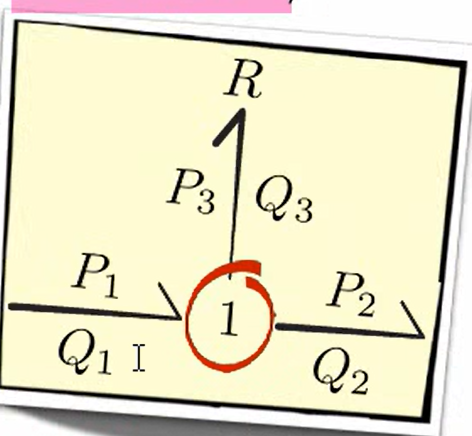
\includegraphics[scale=0.25]{figs/chapter3/3_17.png}
  \caption{Fluid resistor connecting two fluid nodes.}
\end{figure}

\begin{equation*}
  \begin{matrix}
    Q_1 = Q_2 = Q_3 \\
    P_3 = P_1 - P_2 = \Phi_R(Q_3)  = R_3 Q_3 \quad \text{(linear)} 
  \end{matrix}
\end{equation*}

The Reynold number determines if the flow is laminar or turbulent and thus the relationship between pressure drop and flow rate

\begin{equation*}
  Re = \frac{4 \rho Q}{\pi d \mu}
\end{equation*}

\begin{itemize}
  \item If the Reynolds number is low ($Re < 2000$), $P = R Q$, where $R$ is the linear resistance coefficient. This is the regime of laminar flow, where the fluid flows in parallel layers without turbulence.
  \begin{equation*}
    R = 128 \mu l / (\pi d^4)
  \end{equation*}

  \item If the Reynolds number is high ($Re > 5000$), the flow is turbulent, and the pressure drop is given by $P = a_t Q |Q|^{3/4}$, where $a_t$ is a turbulent resistance coefficient.
  
  \item For $2000 < Re < 5000$, the flow is in a transitional regime, and the relationship between pressure drop and flow rate is more complex, often requiring empirical data or more sophisticated models to accurately describe the behavior.

\end{itemize}

\subsubsection{Orifices}
Short obstructions like orifices and valves are important cases where a pressure drop occurs over short lengths. For an orifice with a fixed area, the pressure drop is proportional to the square of the volume flow rate 

\begin{equation*}
  \Delta P = \frac{\rho Q|Q|}{2 C_d^2 A_0^2}
\end{equation*}

where the discharge coefficient $C_d$ depends on the geometry and nonidealities.

\subsubsection{Valves}
For valves, the area $A(x)$ depends on a position coordinate. The position of a mechanical part influences the hydraulic resistance, acting as a transducer linking the mechanical and hydrostatic domains. They can be modeled by variable-resistance elements modulated by a displacement $\dot{x}$.

\begin{equation*}
  \Delta P = \frac{\rho Q|Q|}{ 2 C_d^2(x) A_0^2(x)}
\end{equation*}

It's important to note that elecetrovalevs modeling is a challenging task.

\subsection{Fluid Capacitance}
A fluid capacitor imposes a relationship between a \textbf{pressure and the integral of the volume flow rate}. Essentially is the  volume of fluid.

\begin{figure}[H]
  \centering
  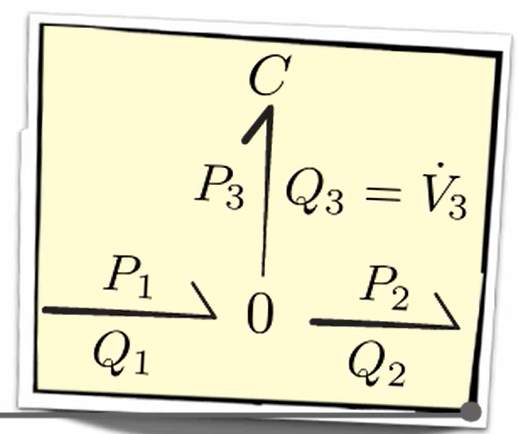
\includegraphics[scale=0.25]{figs/chapter3/3_18.png}
  \caption{Fluid capacitor.}
\end{figure}

\begin{equation*}
  \begin{matrix}
    P_3 = \Phi_C^{-1}(V_3) = \frac{V_3}{C} \\
    V_3 = \int Q_3 dt
  \end{matrix}
\end{equation*}


For a straight-walled water tank in a gravity field,

\begin{equation*}
  P_3 = \rho g h = \rho g \frac{V_3}{A_3}
\end{equation*}
\begin{equation*}
  C_3 = \frac{A_3}{\rho g}
\end{equation*}

\begin{insightbox}[Fluid capacitance as "pressure inertia"]
  The fluid capacitance can be thought as a "Pressure Inertia". Just as a mass resists changes in velocity, a fluid capacitor resists changes in pressure. The larger the capacitance, the more fluid volume is needed to produce a given pressure change, which is analogous to how a larger mass requires more force to achieve the same acceleration.
\end{insightbox}


\subsubsection{Fluid Compressibility}
If and are not equal, represents the rate of compression of the fluid in the pipe. and $V_3$ represents the decrease in volume of the fluid in the segment.

\begin{equation*}
  \begin{matrix}
    dP = - B \frac{dV}{V_0} \\
    \Delta P = \frac{B}{V_0} \Delta V_3 \Longrightarrow C = \frac{V_0}{B}
  \end{matrix}
\end{equation*}

\subsubsection{Elasticity of the vessel}
In the other case, the fluid is incompressible, but the vessel containing it is elastic. The pressure change is related to the change in volume by the bulk modulus of the vessel material. The bulk modulus $B$ is defined as the ratio of the infinitesimal pressure increase to the resulting relative decrease in volume:

The bulk modulus is expressed as:
\begin{equation*}
  B = -V_0 \frac{dP}{dV}
\end{equation*}

\begin{figure}
  \centering
  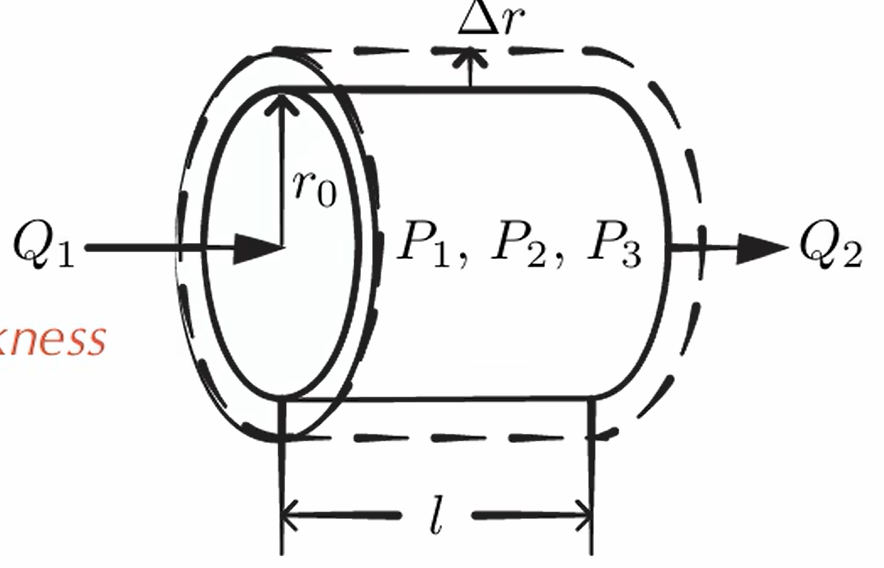
\includegraphics[scale=0.25]{figs/chapter3/3_19.png}
  \caption{Fluid capacitance due to vessel elasticity.}
\end{figure}

\begin{equation*}
  \begin{matrix}
    \sigma = \frac{r_0 P}{t_w} \longrightarrow \text{hoop stress} \\
    \epsilon = \frac{\sigma}{E} = \frac{r_0 P}{t_w E} = \frac{\Delta r}{r_0} \longrightarrow \text{circumferential strain} \\
  \end{matrix}
\end{equation*}

So the change in volume is:

\begin{equation*}
  \begin{matrix}
    \Delta V = \Delta (\pi r^2 l) = \dots = \frac{2 r_0 V_0}{t_w E} P \\
    P_3 = \frac{t_w E}{2 r_0 V_0} V_3 \Longrightarrow C = \frac{2 r_0 V_0}{t_w E}
  \end{matrix}
\end{equation*}

\begin{insightbox}[Capacitance in parallel]
  For cases in which both effect (fluid compressibility and vessel elasticity) contribute, the total capacitance is the sum of the individual capacitances, as they are in parallel. This is because both effects contribute to the overall change in volume for a given pressure change, and their contributions add together to determine the total capacitance of the system.

  \begin{figure}[H]
    \centering
    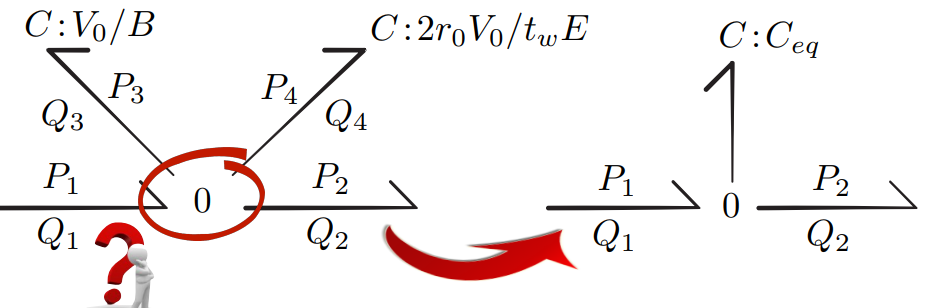
\includegraphics[scale=0.25]{figs/chapter3/3_20.png}
    \caption{Parallel combination of fluid compressibility and vessel elasticity.}
  \end{figure}

  If both fluid compressibility and pipe elasticity contribute, an equivalent compliance can be constructed: $C_{eq} = V_0(\frac{1}{B} + \frac{2r_0}{t_w E})$.

\end{insightbox}


When fluid compliance cannot be modeled with linear behavior, nonlinear models are essential. An example is a gas accumulator with a rubber bladder containing compressed gas. Using the isentropic pressure-volume law 

\begin{figure}[H]
  \centering
  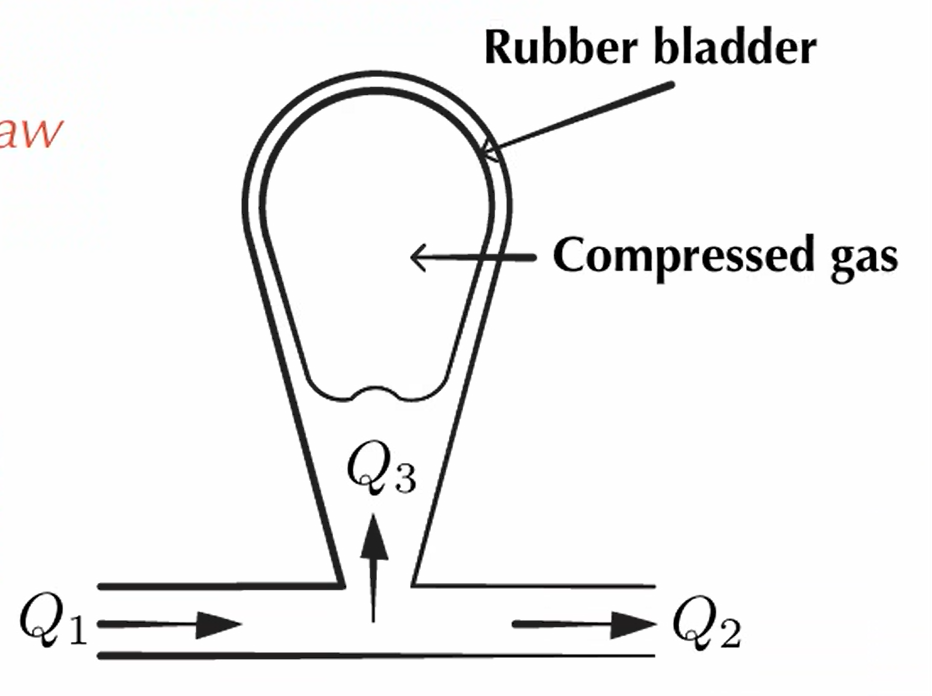
\includegraphics[scale=0.25]{figs/chapter3/3_21.png}
  \caption{Nonlinear fluid capacitor with isentropic behavior.}
\end{figure}

\begin{equation*}
    P V^\gamma = const
\end{equation*}

The pressure is a nonlinear function of the volume: $P_3 = \frac{P_0 V_0^\gamma}{(V_0 - V)^\gamma}$.

\subsection{Fluid Inertia}
Fluid systems have inertia effects analogous to mechanical systems: fluid elements store kinetic energy. The inertia coefficient is related to the parameters of a pipe segment. 

\begin{equation*}
  p_{P_3} = \int P_3 d\tau = \int (P_1 - P_2) d\tau \leftrightarrow I_3 Q_3 = p_{P_3}
\end{equation*}

From Newton's law, a linear inertia coefficient for a pipe of constant cross-section $A$ and length $l$ is $I = \rho \frac{l}{A}$. For a pipe with a non-constant section, $I = \int_0^l \frac{\rho}{A(s)} ds$.

\begin{figure}[H]
  \centering
  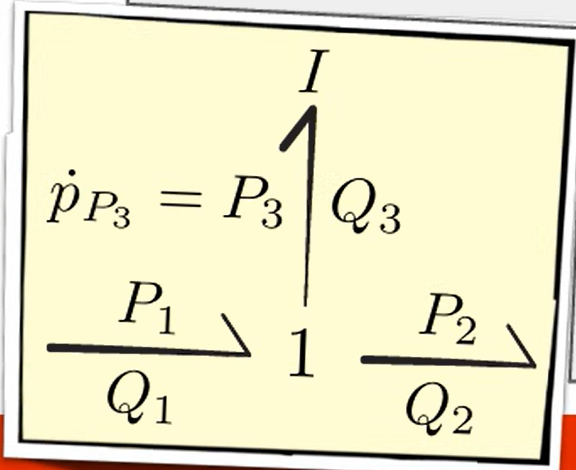
\includegraphics[scale=0.25]{figs/chapter3/3_22.png}
  \caption{Fluid inertia in a pipe segment.}
\end{figure}

\begin{insightbox}[Explaining the fluid inertia]
  The fluid inertia is used to explain the phenomenon that happens when, for instance, a valve is suddenly closed. The fluid in the pipe has kinetic energy (a buildup of momentum), and when the valve is closed, the momentum cannot dissipate immediately, it has to keep flowing until it is dissipated.
\end{insightbox}

\subsubsection{Construction of Hydraulic Bond Graphs}
For both, the construction procedure follows the same 0/1-junction rules as electrical circuits:
\begin{enumerate}
  \item Indicate positive directions for fluid flows and pressures.
  \item For each distinct absolute pressure introduce a 0-junction. Attach elements if they react to one of the absolute pressures. If necessary, include a 0-junction for atmospheric pressure (which can be eliminated if "gauge" pressures are used. Namely, it can be elimnated if all the compoents has a base, the atmospheric pressure).
  \item Insert R-, C-, and I-elements between appropriate 0-junctions using 1-junctions that establish pressure differences acting on the passive elements.
  \item Simplify the graph.
\end{enumerate}

\section{Transducers \& multi-energy domain models}

Transducers are devices that couple subsystems of distinct energy domains. A major reason for studying bond graphs is that they provide a uniform and precise way to represent systems when several forms of power and energy are involved.

\paragraph{Transformer transducers.} 
An ideal transformer transducer, like a hydraulic ram (piston), converts mechanical power to hydraulic power.

\begin{figure}[H]
  \centering
  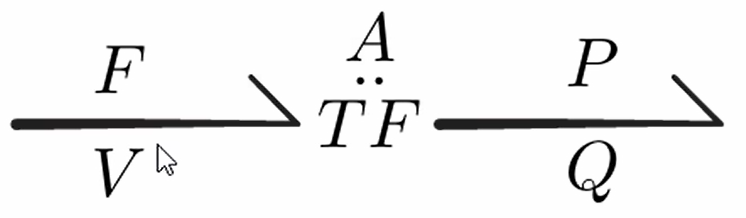
\includegraphics[scale=0.25]{figs/chapter3/3_23.png}
  \caption{Ideal transformer transducer (piston) connecting mechanical and hydraulic domains.}
\end{figure}

\begin{itemize}
  \item Transformer is for the fact that the relation between the two domains is a linear scaling of effort and flow variables. 
  \item Transducer is for the fact that it converts power from one domain to another.
\end{itemize}

\begin{figure}[H]
  \centering
  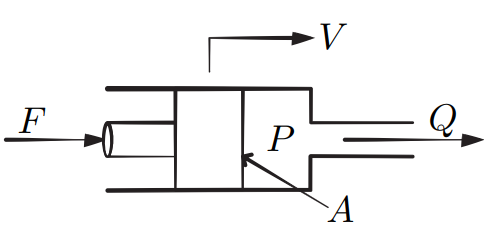
\includegraphics[scale=0.25]{figs/chapter3/3_24.png}
  \caption{Ideal transformer transducer (piston) with idealized power flow.}
\end{figure}

\begin{equation*}
  \begin{matrix}
    F = A P \\
    V = \frac{Q}{A}
  \end{matrix}
\end{equation*}
This applies only to the ideal effects at the face of the piston. Real devices exhibit power losses and energy-storing mechanisms. The process consists of enriching the idealized model. On the mechanical side, we add a 1-junction with a resistor to include friction (which may be dry friction, $F_f = F_0 sgn(V)$, or linear, $F_f = bV$) and an I-element for the piston's mass. On the hydraulic side, a 0-junction and resistance represent leakage, and a C-element models fluid compliance (which may be nonlinear and depend on the nominal extension $x_0$). This complexity can lead to oscillatory phenomena that are damped by the resistance.

\begin{figure}[H]
  \centering
  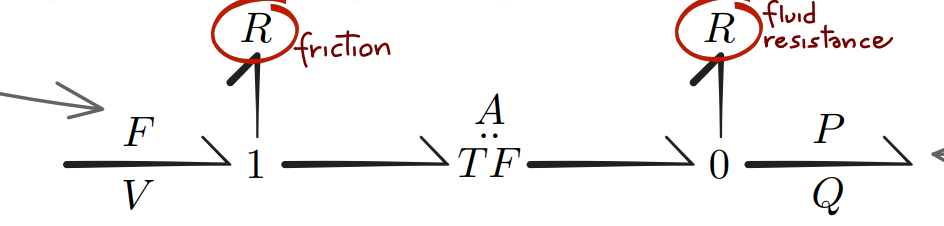
\includegraphics[scale=0.25]{figs/chapter3/3_25.png}
  \caption{Enriched transformer transducer model with losses and energy storage.}
\end{figure}

Positive displacement hydraulic pumps and motors consist of pistons moved by a shaft. With many pistons, the angular speed is related to the flow rate by a nearly constant coefficient: 
\begin{equation*}
  \begin{matrix}
    P_B - P_A = T \tau \\
    T Q = \omega
  \end{matrix}
\end{equation*}

\begin{figure}[H]
  \centering
  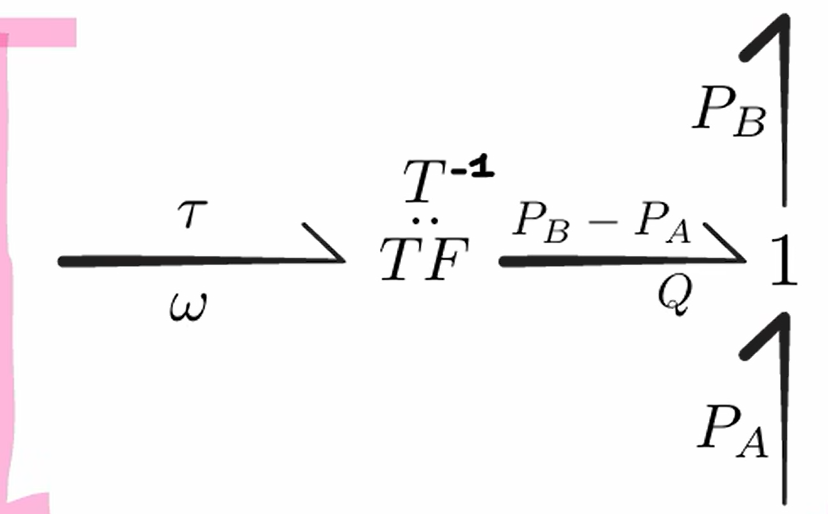
\includegraphics[scale=0.25]{figs/chapter3/3_26.png}
  \caption{Positive displacement hydraulic pump/motor model.}
\end{figure}

  \begin{insightbox}{Enriching the ideal transformer model}
  The ideal transformer model captures the fundamental power conversion mechanism, but it does not account for real-world complexities such as friction, inertia, leakage, and compliance. By enriching the model with additional elements (resistors for losses, I-elements for inertia, C-elements for compliance), we can capture a more accurate representation of the system's behavior. The augmented model can exhibit also non linear phenomena.
  \begin{figure}[H]
    \centering
    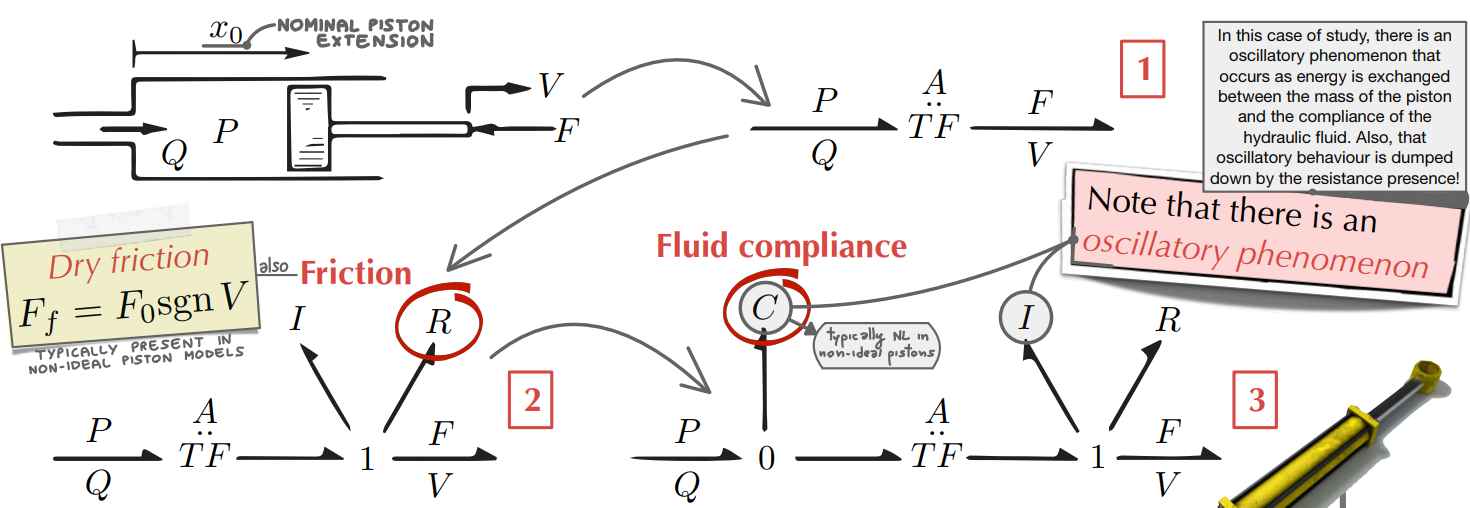
\includegraphics[scale=0.25]{figs/chapter3/3_27.png}
    \caption{Enriched transformer model with additional phenomena.}
  \end{figure}
\end{insightbox}

\paragraph{Gyrator transducers.}
Electromechanical transducers, such as rotary/linear motors or voice coils, use gyrators. A current-carrying conductor moving in a magnetic field experiences an induced voltage (Faraday's law, $e = BlV$) and produces a force (Lorentz force, $Bli = F$). The cross-coupling of effort to flow and flow to effort makes this a gyrator ($e/V = GY = F/i$).

For a DC motor/generator with a commutator, the induced voltage is proportional to the angular speed, and the torque is proportional to the current:

\begin{equation*}
  \begin{matrix}
    e = T \omega \\
    T i = \tau
  \end{matrix}
\end{equation*}

\begin{figure}[H]
  \centering
  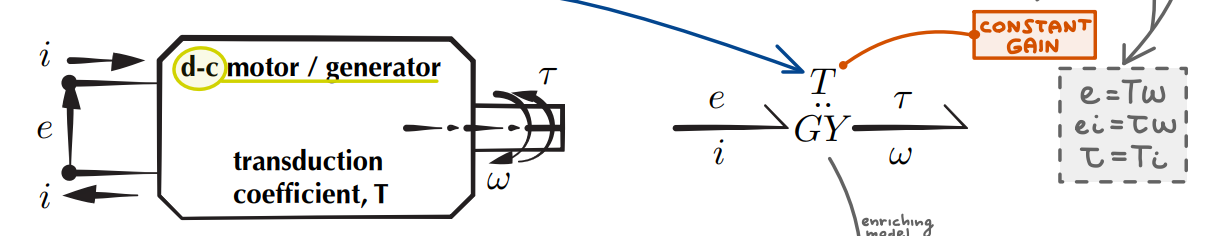
\includegraphics[scale=0.25]{figs/chapter3/3_28.png}
  \caption{Gyrator transducer model for an electromechanical device.}
\end{figure}

A detailed model is developed by adding the winding resistance and inductance, and the rotor's inertia and friction to the basic GY element.

\begin{figure}[H]
  \centering
  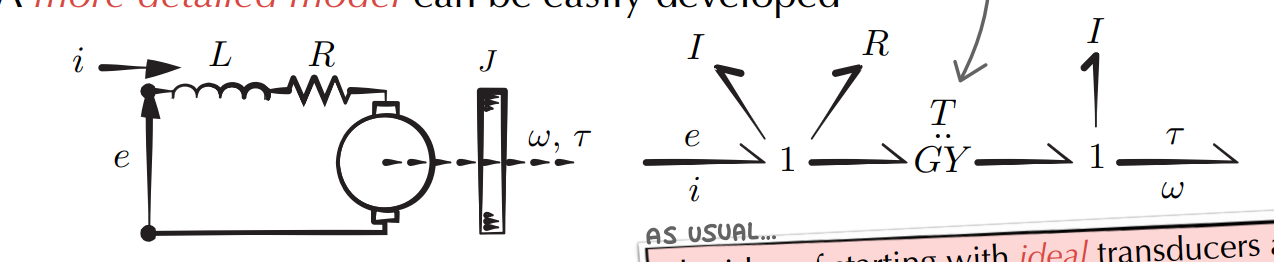
\includegraphics[scale=0.25]{figs/chapter3/3_29.png}
  \caption{Enriched gyrator model with additional phenomena.}
\end{figure}



\paragraph{Modulated Transducers.}
If the gain is time-dependent, MTF and MGY can model more complex power transducers. 

\begin{equation*}
  \left\{\begin{matrix}
    \lambda = n B l_2 l_1 \sin\theta \\
    e = (n B l_2 l_1 \cos\theta) \omega \\
    (n B l_2 l_1 \cos\theta) i = \tau
  \end{matrix}\right.
\end{equation*}

\begin{figure}[H]
  \centering
  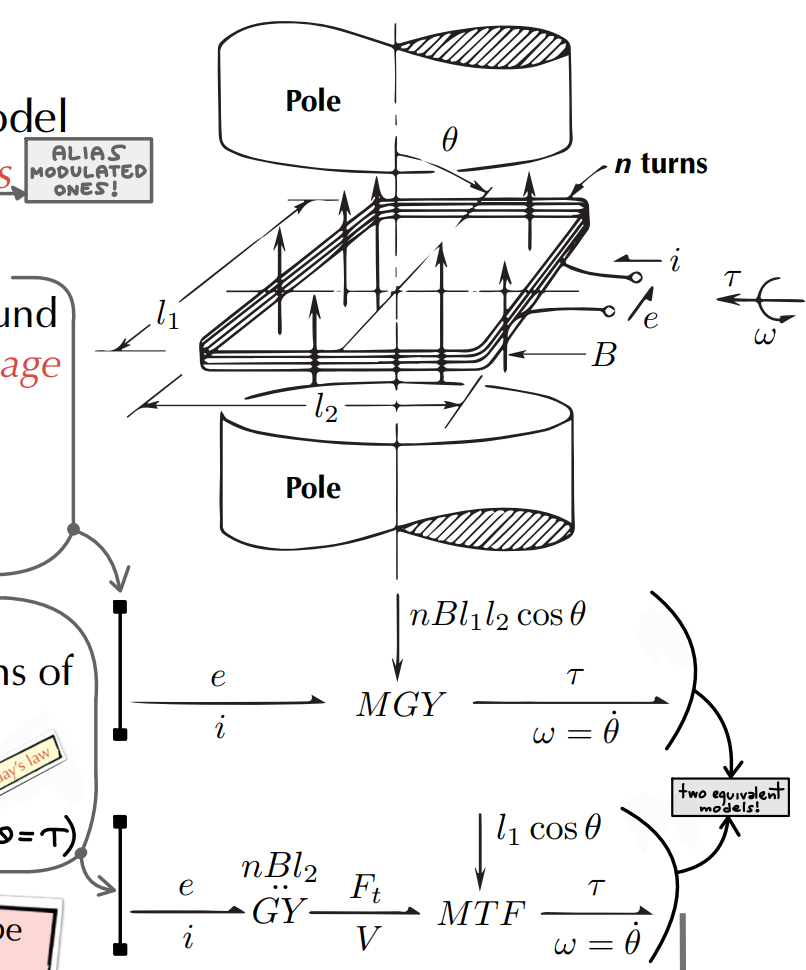
\includegraphics[scale=0.25]{figs/chapter3/3_30.png}
  \caption{Modulated transformer and gyrator transducers.}
\end{figure}

%──────────────────────────────────────────────────────────────────────
\part{Causality, Equations and Advanced Structures}
%──────────────────────────────────────────────────────────────────────
 %%%%%%%%%%%%%%%%%%%%%%%%%%%%%%%%%%%%%%%%%%%%%%%%%%%%%%%%%%%%%%%%%%%%%%%
\chapter{Causality and System Equations}
\label{ch:causality}
%%%%%%%%%%%%%%%%%%%%%%%%%%%%%%%%%%%%%%%%%%%%%%%%%%%%%%%%%%%%%%%%%%%%%%%

In the world of state-space equations, the very same system can be described with different (but equivalent) sets of differential equations. The whole order of the system equations will always be the same (equal to the order of the model). For instance, a system can be represented by a single nth-order differential equation in terms of one unknown variable, or $n$ first-order coupled differential equations in terms of $n$ unknown variables (system theory approach), or various combinations of unknowns and equations of appropriate orders obtained with the Lagrangian approach. 

We aim for a unified and easier methodology: Bond Graphs! One reason for constructing bond graphs is that it is straightforward to derive system equations and to develop numerical simulations. We can also go from a bond graph directly to a simulation without first obtaining the equations of motion manually. The real virtue of bond graph modelling becomes apparent when one considers that all system models use the same symbols. One formulation and solution procedure is needed!

Assigning causality to a bond graph is the step that transforms a structural description into a computational one. It decides which variables are inputs and which are outputs at every port, propagates these choices through the graph, and ultimately determines the mathematical character of the resulting model. The systematic procedure for doing this, the Sequential Causal Assignment Procedure (SCAP), is the workhorse algorithm for deriving state-space equations from bond graphs.

\section{The augmented bond graph}

Before deriving equations, the bond graph must be \textbf{augmented}: 
\begin{enumerate}
  \item The bond graph has been designed, and an appropriate power convention has been assigned.
  \item All bonds are numbered consecutively. This creates the \emph{computational bond graph}.
  \item Each bond is assigned a causal orientation (causal stroke) for the $e$ and $f$ variables.
\end{enumerate}

The causal strokes record, for every bond, whether effort flows left-to-right or right-to-left — i.e.\ which element is computing each variable. The power half-arrow and the causal stroke are completely independent pieces of information. The half-arrow records the assumed positive power direction; the causal stroke records the computational input--output assignment. Do not confuse them. Power sign convention and causality assignment are totally unrelated.

\section{Causality constraints by element type}

In a causal sense, there are two types of bond graph elements: sources ($Se$ and $Sf$) and junctions (0, 1, TF, and GY), that must meet certain causal conditions or their basic definitions are no longer valid. If a system cannot meet these causal conditions, the basic physical model on which the bond graph is based must be restudied; an impossible situation that is not capable of sensible mathematical resolution has been created.

Every element imposes constraints on the causalities of its bonds:
\begin{itemize}[leftmargin=2em,itemsep=3pt]
  \item \textbf{Se}: must impose effort — the causal stroke is always \emph{away} from the Se.
  \item \textbf{Sf}: must impose flow — the causal stroke is always \emph{toward} the Sf.
  \item \textbf{C (integral causality)}: flow is input, effort is output — stroke away from C. A capacitor in integral causality is used as a charge storage and for this it fills having its own voltage.
  \item \textbf{C (derivative causality)}: effort is input, flow is output — stroke toward C. This is the \emph{non-preferred} form. A capacitor in derivative causality is used as a current generator to keep up lacks of voltage by discharging $I=C\dot{V}$.
  \item \textbf{I (integral causality)}: effort is input, flow is output — stroke toward I. An inductor in integral causality is used as a momentum storage and for this it fills having its own current (speed).
  \item \textbf{I (derivative causality)}: flow is input, effort is output — stroke away from I. Non-preferred. An inductor in derivative causality is used as a voltage generator to keep up lacks of current by discharging $V=L\dot{I}$.
  \item \textbf{R}: generally indifferent (either causality), unless the constitutive law is not invertible (e.g.\ Coulomb friction, which is not a bijection in $e$--$f$).
  \item \textbf{TF}: one port effort-in, the other effort-out (one stroke in, one out).
  \item \textbf{GY}: both ports effort-in, or both effort-out (both strokes on the same side).
  \item \textbf{0-junction}: exactly one bond has its effort directed \emph{into} the junction (one stroke pointing away from the junction); all others have effort directed out (stroke toward junction).
  \item \textbf{1-junction}: exactly one bond has its flow directed \emph{into} the junction (one stroke toward junction); all others have flow directed out (stroke away from junction).
\end{itemize}

These constraints mean that once any one element in a connected sub-graph gets its causality assigned, that assignment propagates through junctions and 2-port elements like a chain reaction. The constraint elements represent the physical structure in the system, and assigning causality to them means that they are used correctly in a particular "input-output fashion".

\section{The Sequential Causal Assignment Procedure (SCAP)}

\begin{enumerate}[leftmargin=2em,label=\textbf{Step \arabic*.},itemsep=4pt]
  \item \textbf{Assign source causalities.} For each Se and Sf, assign the only admissible causal form. Propagate the implications through all constraint elements (0, 1, TF, GY) which may be connected to it. 
  \item Repeat step 1 until all sources have been assigned the required causality.
  \item \textbf{Assign storage elements (preferred causality).} For each C and I element not yet causally assigned, assign \emph{integral causality} (preferred). Propagate through constraint elements. 
  \item Repeat step 3 until all storage elements have been assigned a causality. 
  \item \textbf{Assign R-elements (if still needed).} If bonds remain unassigned after steps 1--4, choose any unassigned R-element and assign an arbitrary causality to it, and extend the causal implications through the graph. Each such arbitrary assignment signals an \textbf{algebraic loop}. 
  \item Repeat step 5 until all R-elements have been used.
  \item \textbf{Assign remaining bonds arbitrarily.} Any remaining unassigned bond (joined to two constraint elements) can be assigned arbitrarily. Extend the causal implications. Each produces another algebraic loop.
  \item Repeat step 7 until all remaining bonds have been assigned.
\end{enumerate}

The procedure is straightforward and orderly, and it can be implemented in a simulation environment. Note that in assigning causality, the results do not depend on the order of bonds chosen (except in special circumstances).

\begin{insightbox}[What the SCAP tells you]
Several situations can arise when applying the SCAP, revealing the type of mathematical model:
\begin{itemize}[leftmargin=1.5em,itemsep=0pt]
  \item \textbf{All storage elements in integral causality, and the graph is complete after step 4}: the simplest and most common case. The model yields explicit ODEs directly.
  \item \textbf{Causality is completed using steps 5-8}: one or more \emph{algebraic loops} exist. The model involves coupled algebraic--differential equations; some effort or flow variable is algebraically related to itself and must be solved simultaneously.
  \item \textbf{Some storage elements forced into derivative causality (during step 3)}: the model contains \emph{implicit} differential equations (DAEs). The number of derivative-causality storage elements equals the \emph{reduction in system order} relative to the total element count.
\end{itemize}
\end{insightbox}

\section{Reading off state-space equations: Basic formulation \& Reduction}

From a fully augmented bond graph model, the equations for the system can be developed in a very orderly fashion, either by hand or thanks to a simulation package. Very general and powerful procedures are available for producing sets of system equations, consisting of these main steps: select input and energy state variables, formulate the initial set of system equations, and reduce the initial equations to state-space form.

The selection of inputs is straightforward, since they are associated to each source element. These variables will appear in the final state-space equations if they have any effect on system behaviour.

The state variables are:
\begin{itemize}[leftmargin=2em,itemsep=0pt]
  \item The \textbf{momentum $p$} on every I-element in \emph{integral} causality.
  \item The \textbf{displacement $q$} on every C-element in \emph{integral} causality.
\end{itemize}

It is useful to indicate the \textbf{co-energy variables}: flows on the I-elements ($f = \Phi_I^{-1}(p)$) and efforts on the C-elements ($e = \Phi_C^{-1}(q)$). Co-energy variables appear in the initial formulation and then they are eliminated during the reduction process since they are function of the state.

The order of the system equals the number of energy storage elements in integral causality. The derivation procedure is systematic:

\begin{enumerate}[leftmargin=2em,label=\textbf{(\arabic*)},itemsep=3pt]
  \item For each state variable, write its rate of change (time derivative) as an effort or a flow: $\dot{p} = e$ or $\dot{q} = f$.
  \item Causality is used to track the efforts and flows through the bond graph. The causal stroke tells us which element is \emph{providing} this effort or flow. Trace through the bond graph from the state variable's bond, substituting at each junction and element, until only sources and \textbf{co-energy variables} remain. It makes no difference which state variable we start with.
  \item Substitute the co-energy variables last to obtain equations purely in state variables and inputs. This leads to explicit first-order equations.
\end{enumerate}

\figplaceholder{Example 1: Formulation of a simple 2-state system}{See slides 18-19, pack M04}

\begin{mathbox}[Simple example: RC circuit]
State variable: $q_2$ on C. Input: $e_1(t)$ from Se.\smallskip

From the 0-junction: $e_2 = e_1 - e_4$ (0-jct, effort balance).\newline
From the 1-junction: $e_4 = R_4 f_4 = R_4 f_2$ (R-element, effort-in causality, same flow on 1-jct).\newline
Co-energy: $f_2 = \dot{q}_2$, and $e_2 = q_2/C_2$.\medskip

Result: $\dot{q}_2 = f_2 = \frac{e_1 - q_2/C_2}{R_4}$ — the standard RC first-order equation.
\end{mathbox}

\paragraph{The 1-junction encodes KVL, the 0-junction encodes KCL.}
Reading equations from a bond graph is essentially applying Kirchhoff's laws automatically: the 0-junction says ``efforts sum to zero around a node'' (I Kirchhoff); the 1-junction says ``flows sum to zero around a loop'' (V Kirchhoff). Causality tells you which variable is expressed in terms of the others.

\figplaceholder{Example 3: System with a transformer and multiple states}{See slides 20-23, pack M04}

\section{Algebraic loops}

Talking about state-space equations formulation, in situations in which we do NOT have algebraic-loops and we have ALL storage energy elements in integral causality, the formulation is very straight-forward, obtaining explicit differential equations. Instead, when we have algebraic loops (we have encountered steps 5-6 of the SCAP) and/or we have some energy storage elements in derivative causality, the formulation is not anymore so immediate! 

An algebraic loop arises when a chain of elements forms a closed ring with no energy-storage element breaking it. In that loop, one variable (effort or flow) becomes algebraically related to itself (as well as to other inputs and co-energy state variables). Tracing around the loop brings you back to your starting point: $e_1 = F_1(e_2, f_2)$, $e_2 = F_2(e_3, f_3) \dots$ until we reach again the initial variable.

The procedure for handling algebraic loops is to first make an arbitrary causal assignment on one of the causally unassigned bonds and then propagate the causal information as far as possible. If the causality completes after one arbitrary assignment, then there is one algebraic loop. The more loops involved, the more difficult the final formulation becomes.

\begin{warningbox}[Cause of algebraic loops]
Algebraic loops always arise from a \textbf{modelling simplification}. For example, two parallel dampers with no masses to separate them create an algebraic loop in force. In reality, there would be some small compliance or inertia in between; the idealisation of perfectly rigid connections removes it and creates the loop. 
\end{warningbox}

When SCAP is stuck on step 4, it is necessary to arbitrarily assign causality to one bond. It is recommended that when a resistance element is involved in the algebraic loop, the resistance element be chosen for the arbitrary assignment (step 5). It is customary to choose the variable that was arbitrarily selected to be the output from the R-element and the input to the rest of the system. 

In order to solve the algebraic loop, we have to collect all the equations involved in the loop and solve the system to find an expression of $e/f$ that depends \emph{only} on inputs and/or co-energy state variables. This explicit algebraic equation can then be substituted directly into the ODEs.

For linear systems, this procedure will work for multiple loops, although solving by hand becomes formidable rather quickly. For nonlinear systems, it may not be possible to invert some of the algebraic relationships (e.g. Coulomb friction). When these inversions appear to be impossible, we HAVE TO eradicate the problem at the root by passing to less simplistic modelling assumptions!

\figplaceholder{Algebraic Loop Example: Assigning arbitrary causality on an R-element}{See slides 26-29, pack M04}

\section{Derivative causality}

Another possible consequence of certain modelling assumptions is that, after sequential causal assignment, one or more energy storage elements are forced into derivative causality. 
When a C-element is forced to accept derivative causality (effort-in), it means that its effort (and hence its displacement $q = Ce$) is \emph{algebraically determined} by the rest of the system — it does not contribute an independent state variable to the final equations. This occurs when two C-elements are connected in a configuration that rigidly constrains their displacements (e.g.\ two springs rigidly connected without an intervening mass). The system order is reduced by one per derivative-causality C.

Similarly for I-elements in derivative causality (flow-in): their momenta are algebraically determined. The independent state variables remain the energy variables in the energy storage elements with integral causality. (Note: The derivative elements do still store energy!).

The true problem arises when formulating the equations. When we encounter a C/I element in derivative causality, we are guaranteed to end up with its power variable that is NOT the co-energy one ($\dot{q}$ for C-elements and $\dot{p}$ for I-elements). We end up with a double problem: we end up with the derivative of an energy variable, AND this energy variable is NOT a state one!

These situations always signal an \textbf{implicit (DAE) model}. Implicit state equations can be algebraically transformed to explicit ones, but this is not necessarily a simple task. 

\paragraph{Handling Derivative Causality Algebraically:}
Given the dependent energy variable of a C/I element in derivative causality, it is always guaranteed that it is algebraically related (constrained) to variables that are independent state ones. 
\begin{enumerate}
    \item Find out (by inspecting the BG) the algebraic relation that gives the energy dependent variable as a function of the state ones.
    \item Differentiate that relation to obtain an expression for $\dot{q}$ (for C) or $\dot{p}$ (for I) as a function of differentiated state variables.
    \item Substitute this back into your equations. The result is a valid state equation, but it will be in implicit form.
    \item To get it in explicit form, further algebraic manipulations are required to isolate the derivatives of the state variables on the left side.
\end{enumerate}

\figplaceholder{Derivative Causality Example: Neglecting motor inertia}{See slides 34-36, pack M04}

\paragraph{Handling Derivative Causality at the Root:}
Derivative causality is ALWAYS caused by too simplistic modelling assumptions! It physically indicates an over-idealisation (e.g.\ perfectly rigid connections between compliant elements, or massless inertial elements). 

It is always possible to revisit the modelling assumptions that resulted in the formulation problem and change these assumptions to yield a model that is virtually the same as the original one, but without the formulation problems. Introducing a new energy storage element (a tiny mass or compliance) restores integral causality and ordinary ODE structure. 

There are some computational penalties that accompany very small added inertias or very stiff added compliances in a model (it introduces a fast time scale, making the system "stiff" for numerical solvers). However, for some systems, these penalties are a very small price to pay for eliminating formulation problems at the root.

\section{System order and physical meaning}

The order of a bond graph model equals the number of independent energy storage elements. This is a fundamental invariant: it does not matter which set of state variables is chosen (positions vs.\ momenta, etc.) — the order is always the same. Equivalently, the order equals the minimum number of initial conditions needed to uniquely determine future evolution.

The energy of the system at any instant is the sum of the energies stored in all elements with integral causality:
\begin{equation}
  E_{\mathrm{total}}(t) = \sum_{C\text{-elements}} E_C(q) + \sum_{I\text{-elements}} E_I(p).
\end{equation}
This is the \textbf{Hamiltonian} of the system (in the linear case, $E = \frac{1}{2}\mathbf{x}^T Q \mathbf{x}$ for an appropriate positive-definite matrix $Q$).
 %%%%%%%%%%%%%%%%%%%%%%%%%%%%%%%%%%%%%%%%%%%%%%%%%%%%%%%%%%%%%%%%%%%%%%%
\chapter{Multiport Fields and Junction Structures}
\label{ch:fields}
%%%%%%%%%%%%%%%%%%%%%%%%%%%%%%%%%%%%%%%%%%%%%%%%%%%%%%%%%%%%%%%%%%%%%%%

Real physical components often couple multiple energy flows simultaneously. A flexible beam deformed by two forces stores energy that depends on \emph{both} displacements simultaneously, not independently. A 3D rigid body has coupled translational and rotational inertia. These multi-port couplings cannot be captured by separate 1-port elements — they require \textbf{multiport fields}. 

Using fields and junction structures, it is possible to study systems with complex multiport components using bond graphs because they combine structural detail, clarity, and ease of visualization. 

\begin{insightbox}[Important Assumption for Fields]
All multiport elements that we are going to study in this chapter are assumed to be (and are going to be studied as) \textbf{ALL INWARDS} in terms of power bond directions. This means power is conventionally positive when flowing into the field from all ports.
\end{insightbox}

\section{C-fields: multiport potential energy storage}

A \textbf{C-field} is the multiport generalization of the 1-port C-element. It is itself a distributed compliance element, representing a distributed hole of energy conservation. It has $n$ ports, and its potential energy is a function of all $n$ displacements simultaneously:
\begin{equation}
  E(\mathbf{q}) = \int_{0}^{t} \sum_{i=1}^{n} e_i f_i d\tau = 
  \int_{0}^{t} \sum_{i=1}^{n} e_i \dot{q}_i d\tau = 
  \int_{0}^{t} \sum_{i=1}^{n} e_i(\mathbf{q}) dq_i =  
  \int_{\mathbf{q}_0}^{\mathbf{q}} \mathbf{e}(\bar{\mathbf{q}})^T\,d\bar{\mathbf{q}}, \qquad
  e_i = \frac{\partial E}{\partial q_i}(\mathbf{q}).
\end{equation}

This means that a change in any component is going to cause a change in the stored energy. Because $E(\mathbf{q})$ represents stored potential energy, the C-field inherently conserves energy.

\begin{insightbox}{Advantage of Fields}
  The advantage of Fields is that they allow us to capture the physics of multiport energy storage directly, without needing to break it down into multiple 1-port elements and junctions. Moreover, a C-field can be thought of as a \textbf{Inertia} \textbf{Compliance} \textbf{Damping} Matrix that captures the coupling between ports in a compact way without the need of explicitly writing the internal structure of the filed. 
\end{insightbox}


The constitutive law is a set of $n$ functions $e_i(\mathbf{q})$ giving the efforts at each port as a function of all displacements. By inspection, $\mathbf{e}(\mathbf{q}) = \nabla E(\mathbf{q})$. For the C-field to be physically meaningful (\textbf{conservative}), the energy function $E(\mathbf{q})$ must exist, which requires the \textbf{Maxwell reciprocal relations} (a structural constraint):
\begin{equation}
  \frac{\partial e_i}{\partial q_j} = \frac{\partial^2 E}{\partial q_i \partial q_j} = \frac{\partial e_j}{\partial q_i} \quad \forall\, i,j.
  \label{eq:maxwell}
\end{equation}
This is the direct multivariable generalization of the single-port condition $e = \partial E/\partial q$. It is clear that not every arbitrary set of constitutive laws expressing efforts in terms of displacements could come from a valid energy-storing C-field—only those sets that obey this symmetry property!

\paragraph{Compliance and stiffness forms.}
If the constitutive law can be written $\mathbf{q} = \mathbf{M}_c(\mathbf{e})$ (displacements as functions of efforts), this is the \textbf{compliance form}. If it can be written $\mathbf{e} = \mathbf{M}_k(\mathbf{q})$ (or $\mathbf{M}_c^{-1}(\mathbf{q})$), this is the \textbf{stiffness form}. 

In the linear case, the equations become:
\begin{equation}
  \mathbf{e} = \mathbf{K}\,\mathbf{q} \quad (\text{stiffness}), \qquad
  \mathbf{q} = \mathbf{C}\,\mathbf{e} \quad (\text{compliance}),
\end{equation}
where $\mathbf{K} = \mathbf{C}^{-1}$ is the stiffness matrix and $\mathbf{C} = \mathbf{M}_c$ is the compliance matrix. The stored energy is $E = \frac{1}{2}\mathbf{q}^T\mathbf{K}\mathbf{q}$. Maxwell reciprocity requires $\mathbf{K} = \mathbf{K}^T$ and $\mathbf{C} = \mathbf{C}^T$ (symmetric matrices), a familiar result from structural mechanics.

\begin{example}[Elastic beam loaded at two points]
An Euler-Bernoulli beam of length $L$, stiffness $EI$, loaded by forces $F_1$ at $L/3$ and $F_2$ at $2L/3$ has the compliance matrix:
\begin{equation}
  \begin{pmatrix}x_1\\x_2\end{pmatrix}
  = \frac{L^3}{243EI}\begin{pmatrix}4&\frac{7}{2}\\\frac{7}{2}&4\end{pmatrix}
  \begin{pmatrix}F_1\\F_2\end{pmatrix}.
\end{equation}
The symmetric compliance matrix confirms Maxwell reciprocity. 
\end{example}


\paragraph{Nonlinear C-fields.}
Nonlinear C-fields are common in certain application areas. A mechanical element that behaves as a linear 1-port in restricted cases can often be modelled as a nonlinear 2-port C-field when two-dimensional motion is permitted. 

\begin{figure} [H]
  \centering
  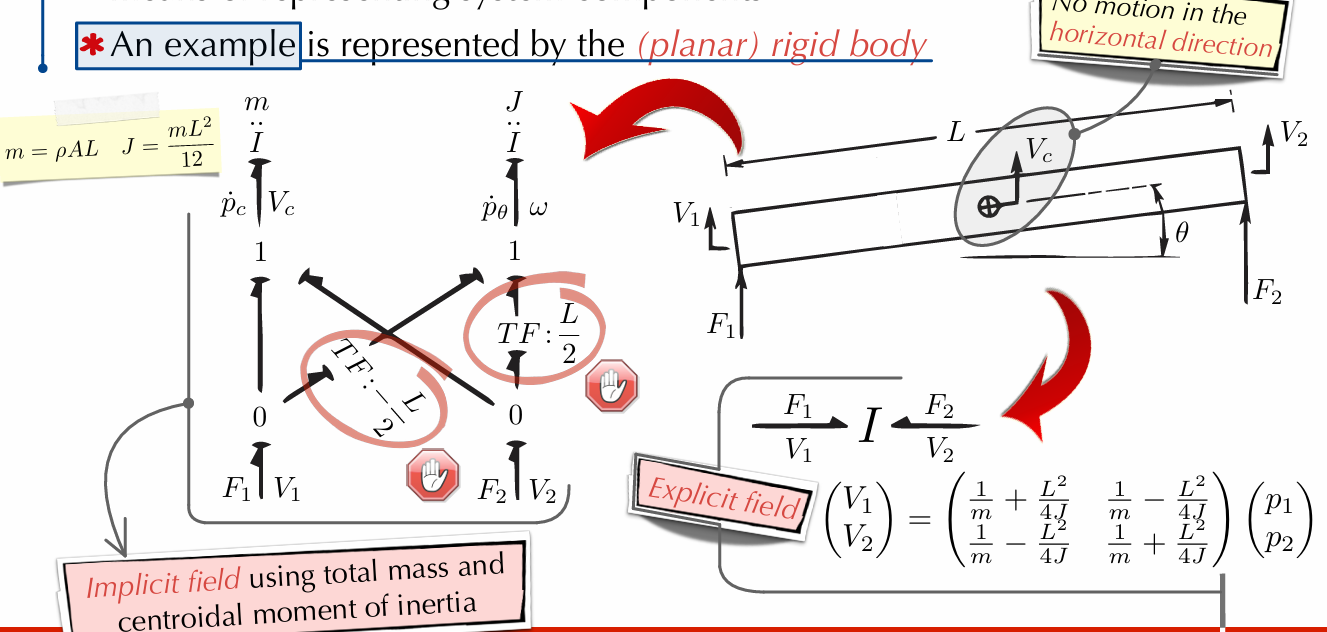
\includegraphics[scale=0.25]{figs/chapter5/5_3.png}
  \caption{A simple linear spring pivoting in a 2D plane is a nonlinear C-field.}
\end{figure}


For example, a simple linear spring (rest length $L_0$, stiffness $k$) pivoting in a 2D plane ($x, y$) has the energy:
\begin{equation}
  E(x,y) = \frac{1}{2}k\left(\sqrt{x^2+y^2} - L_0\right)^2
\end{equation}
The gradient of this potential energy gives the highly nonlinear constitutive equations for the $x$ and $y$ efforts:
\begin{equation}
  F_x = kx - k\frac{L_0 x}{\sqrt{x^2+y^2}}, \qquad F_y = ky - k\frac{L_0 y}{\sqrt{x^2+y^2}}
\end{equation}

\subsection{Explicit vs.\ implicit C-fields}

An \textbf{implicit field} arises when a group of 1-port C-elements, connected by junction structures (0-junctions, 1-junctions, TF), collectively behaves as a C-field. For example, two springs $k_1$ and $k_2$ connected in series via a 1-junction (sharing a common force, but adding displacements) or connected in parallel via a 0-junction form an implicit C-field. The implicit form is naturally obtained from the assembly of the bond graph; converting it to explicit form requires solving for the field's constitutive equations algebraically.

\begin{figure}[H]
  \centering
  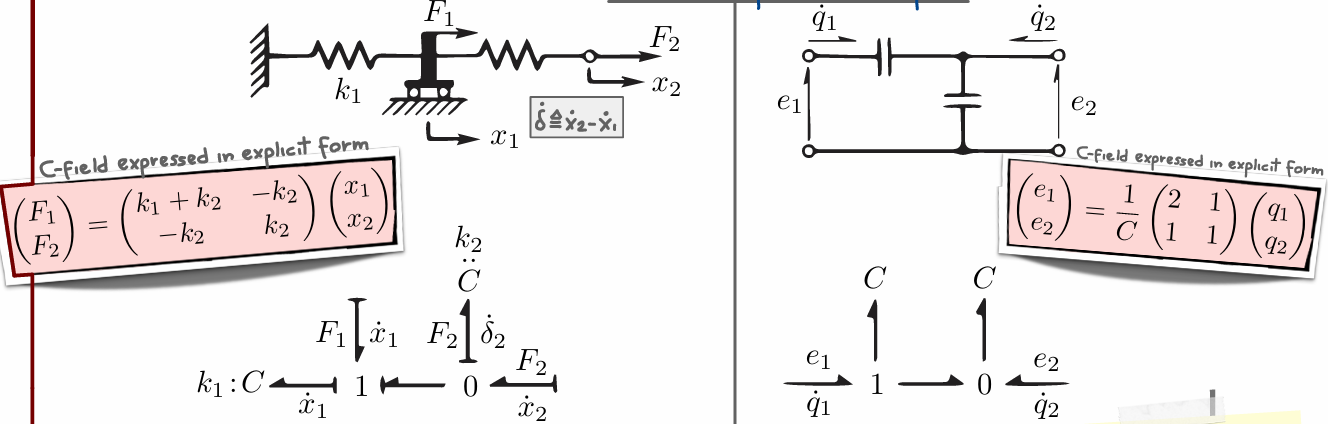
\includegraphics[scale=0.25]{figs/chapter5/5_1.png}
  \caption{Implicit C-field}
\end{figure}

An \textbf{explicit field} is one whose constitutive law is given directly as $\mathbf{e}(\mathbf{q})$ or $\mathbf{q}(\mathbf{e})$ — the multiport is defined from the outset as a single entity (like the beam example above). 

\begin{figure}[H]
  \centering
  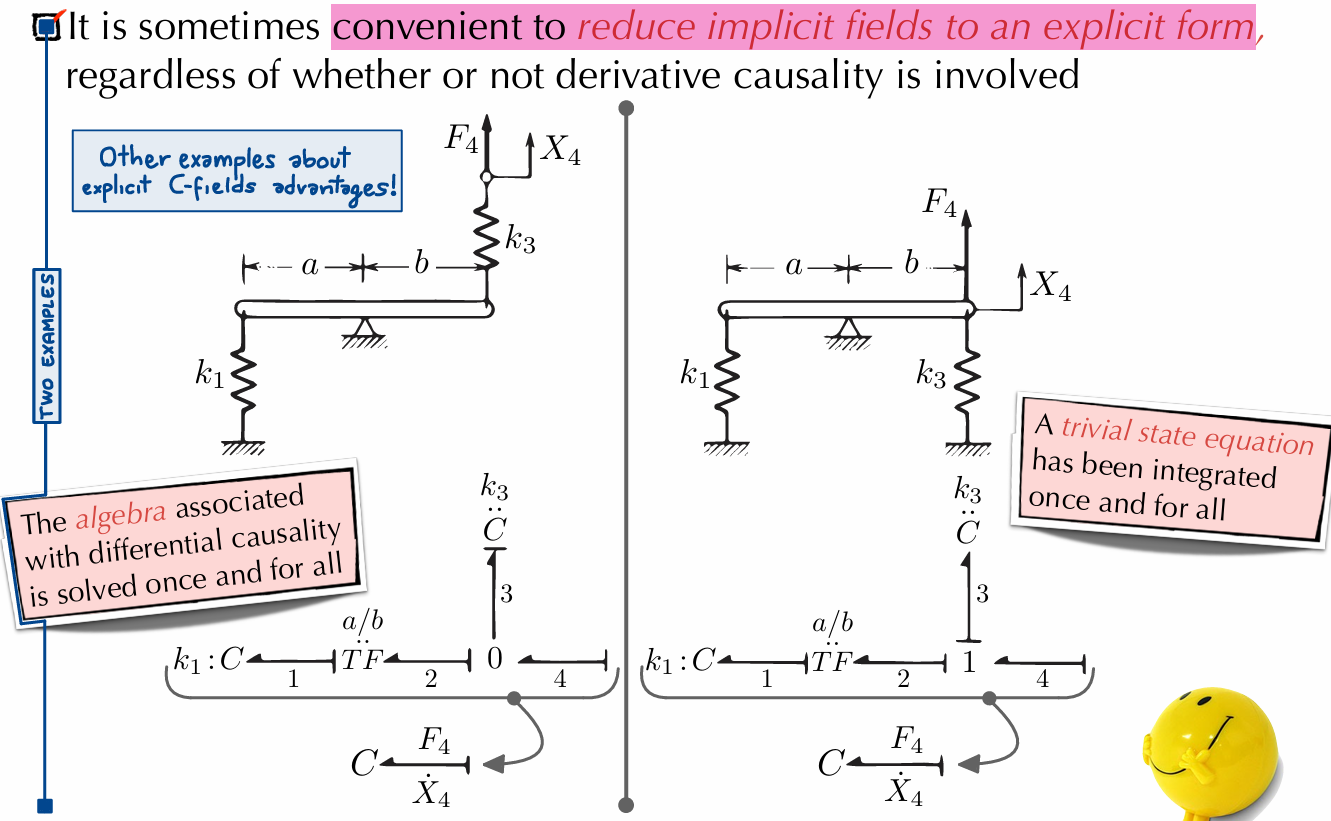
\includegraphics[scale=0.25]{figs/chapter5/5_2.png}
  \caption{Explicit C-field}
\end{figure}


\begin{insightbox}[When to convert implicit to explicit]
  Converting an implicit field to an explicit form (Viva Explicit C-Fields!) is extremely useful when: 
  (a) Some elements of the field are forced into derivative causality. By pre-solving the algebraic loops and constraints inside a field matrix, you save the computer from crashing during simulation and kill the derivative causality mathematically.
  (b) Equation formulation is simplified by working directly with the field's stiffness or compliance. The transformation into an explicit form integrates trivial state equations once and for all, avoiding the necessity of handling derivative causality completely.
\end{insightbox}

\subsection{Causality in C-fields}

As in the case of 1-port C-elements, multiport C-fields also admit mixed integral-derivative causalities. A C-field with $n$ ports can accept any mixture of integral and derivative causalities across its ports, as long as the resulting constitutive equations can be inverted appropriately.

\begin{figure} [H]
  \centering
  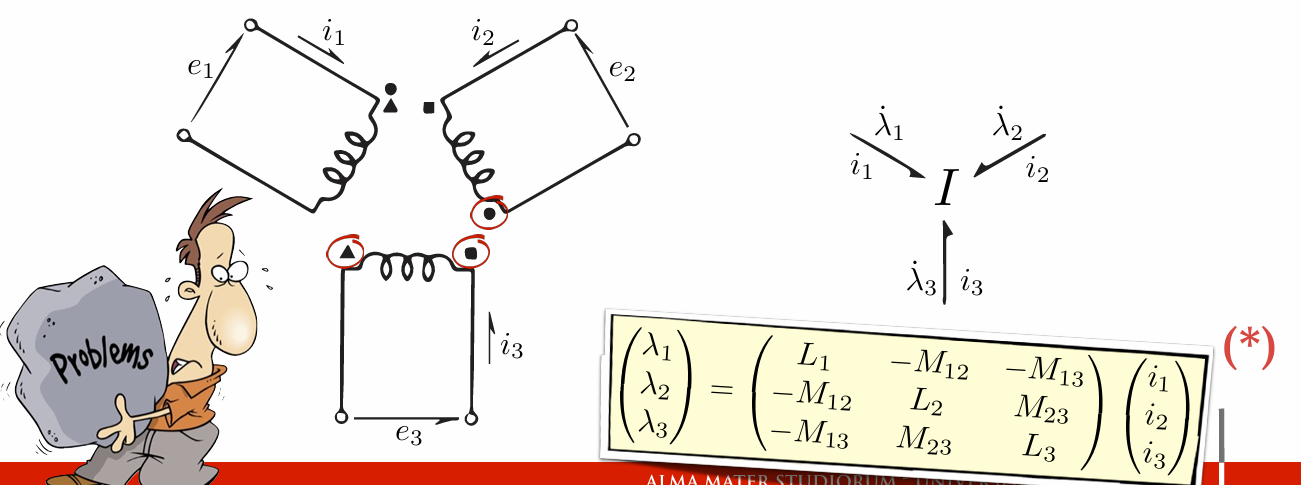
\includegraphics[scale=0.25]{figs/chapter5/5_4.png}
  \caption{Causality in C-fields}
\end{figure}




\begin{insightbox}[Example of causality assignment in a C-field]
  \begin{enumerate}
    \item Draw bond graph
    \item Assign causality
    \item Express the C-field
  \end{enumerate}

  \begin{figure}[H]
    \centering
    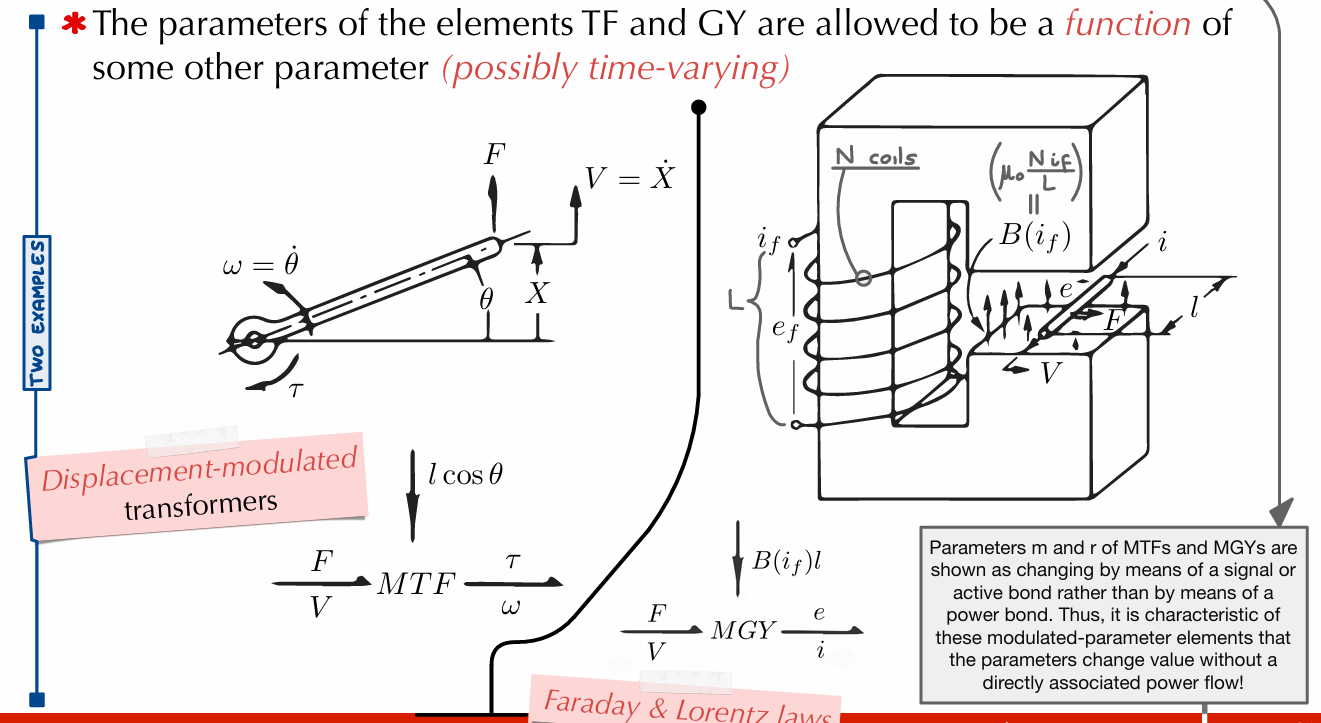
\includegraphics[scale=0.25]{figs/chapter5/5_5.png}
    \caption{Example of causality assignment in a C-field}
  \end{figure}

  The manipulation from implicit to explicit field can be of help if one or more elements must be assigned derivative causality.

  \begin{itemize}
    \item The transformation in an explicit form simplifies equation formulation
    \item This process increases the insight into the \textbf{causes} of derivative causality
    \item The explicit-field representation can be used to avoid the necessity of handling derivative causality. 
  \end{itemize}

  

  It's important to note that when assigning causality, even if an element is assigned in derivative causality, it does not necessarily mean that the resulting constitutive equations will be in derivative form. The derivate causallity of the element is holded inside the C-field, but not externally, at the terminal side. From the terminal point of view, this is just a C-field in fully integral causality. 

  The causality of the inner elements it is not visible from the outside. This is a key point to understand when working with fields.
  
\end{insightbox}


In \textbf{fully integral causality}, all flows are inputs and all efforts are outputs: $\mathbf{e} = \mathbf{K}\,\mathbf{q}$ (stiffness form). In \textbf{fully derivative causality}, all efforts are inputs and all displacements are outputs: $\mathbf{q} = \mathbf{C}\,\mathbf{e}$ (compliance form). \textbf{Mixed causality} involves both, requiring a mixed-form constitutive law obtained by partially inverting the stiffness/compliance matrix. 

For an implicit field, admissible causal forms are easily determined by propagating the standard bond graph causality rules through its constituent elements (e.g., studying conflicts at 0 or 1 junctions). For an explicit field specified in a particular causal form, the question is an algebraic one (whether the constitutive equations can be inverted), and for nonlinear fields, this can be very hard to decide. Notice that, in principle, any strictly valid C-field can always go into fully integral causality!

\section{I-fields: multiport kinetic energy storage}

For I-fields we can develop a complete parallel dual formulation with respect to C-fields. Inertial fields are the exact duals of capacitive fields. The \textbf{I-field} is the multiport generalisation of the 1-port I-element. Its kinetic energy is a function of all momenta simultaneously:

\begin{equation}
  E(\mathbf{p}) = \int_{0}^{t} \sum_{i=1}^{n} e_i f_i d\tau = 
  \int_{0}^{t} \sum_{i=1}^{n} f_i \dot{p}_i d\tau = 
  \int_{0}^{t} \sum_{i=1}^{n} f_i (\mathbf{p}) dp_i =  
  \int_{\mathbf{p}_0}^{\mathbf{p}} \mathbf{f}(\bar{\mathbf{p}})^T\,d\bar{\mathbf{p}}, \qquad
  f_i = \frac{\partial E}{\partial p_i}(\mathbf{p}).
\end{equation}


In the linear case, the energy is $E(\mathbf{p}) = \frac{1}{2}\mathbf{p}^T\mathbf{M}^{-1}\mathbf{p}$. The constitutive law maps momenta to flows via the inverse mass/inertia matrix $\mathbf{M}^{-1}$ (i.e. $\mathbf{f} = \mathbf{M}^{-1}\mathbf{p}$). 

The Maxwell reciprocal relations for I-fields require $\partial f_i/\partial p_j = \partial f_j/\partial p_i$, which translates to the symmetry of $\mathbf{M}^{-1}$ (and hence of $\mathbf{M}$). Like C-fields, I-fields occur in both implicit and explicit forms, and manipulating them can yield highly useful simplified representations.

The most important mechanical physical I-field is the \textbf{3D rigid body}: it has three translational and three rotational momentum ports, with the (constant) mass-inertia tensor providing the constitutive law. In 2D, the I-field reduces to two translational inertias and one rotational inertia, as discussed in Chapter~3. By transforming an implicit rigid-body I-field into an explicit one, we can define the relationship between the center-of-mass velocity and the velocities of the attachment points analytically.


\paragraph{Interacting Coils (Mutual Inductance).}
Another classic use of I-fields is in electrical circuits containing mutually interacting coils. These are conveniently represented using explicit I-fields in derivative causality. To write the constitutive laws, one needs a sign convention for currents/voltages and a convention for the relative orientation of the coils (often denoted by dots, squares, or triangles on schematic diagrams).

If the currents $i_1$ and $i_2$ are defined so that when positive they both enter the dotted ends, the mutual-inductance effects $M$ are positive:
\begin{equation}
  \begin{pmatrix}\lambda_1\\\lambda_2\end{pmatrix} = \begin{pmatrix}L_1 & M_{12}\\ M_{12} & L_2\end{pmatrix}\begin{pmatrix}i_1\\i_2\end{pmatrix}
\end{equation}
If one current enters a dot and the other leaves a dot, the mutual terms become $-M_{12}$. Independently of the coil orientation convention, the inductance matrix and its inverse will always be symmetric as long as the I-field is conservative.

\begin{figure}[H]
  \centering
  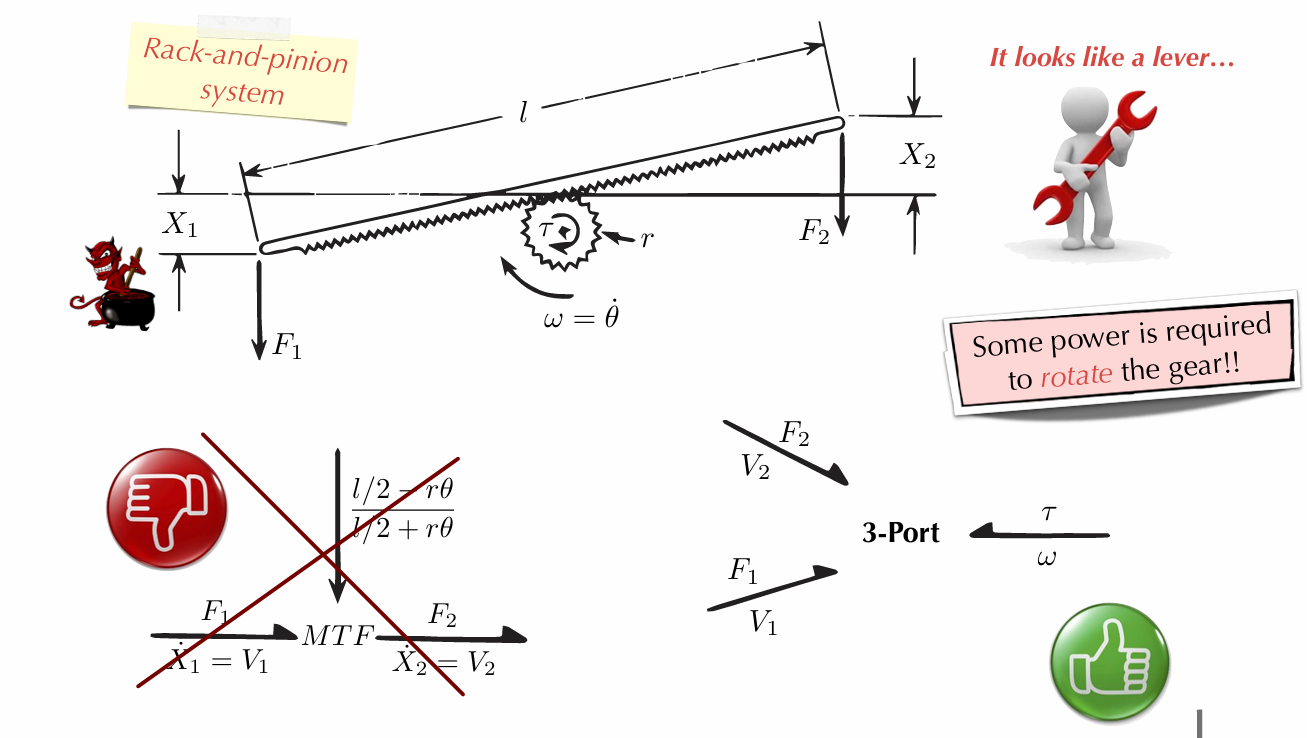
\includegraphics[scale=0.25]{figs/chapter5/5_6.png}
  \caption{Mutually interacting coils represented as an I-field}
\end{figure}


\section{Mixed energy-storing fields (IC-fields)}

There are cases when an energy-storing device acts as a C-field at some ports and an I-field at others. Within a single energy domain, there is usually no need for such an element. However, energy transducers are often ideally energy conservative but store and release energy across different domains over time (e.g., storing electrical energy and releasing it as mechanical work). Because their electrical and mechanical energies are dynamically coupled, they cannot be modeled by simple 1-port C or I elements. You must use a mixed \textbf{IC-field} to mathematically capture the complex physics natively.


For an IC-field with momentum variables $p$ and displacement variables $q$, the total energy features dynamic coupling (an irrotational case) and contains mixed terms. The constitutive equations are obtained by taking the appropriate partial derivatives of the total stored energy $E(p, q)$. 

\begin{equation}
  E(\mathbf{p}) = \int_{0}^{t} \sum_{i=1}^{n} e_i f_i d\tau = 
  \int_{0}^{t} \sum_{i=1}^{j} f_i \dot{p}_i d\tau + \int_{0}^{t} \sum_{k=j+1}^{n} e_k \dot{q}_k d\tau
\end{equation}

Maxwell's reciprocal relations for IC-fields require that the mixed second derivatives of the energy function are equal:
\begin{equation}
  \frac{\partial^2 E}{\partial p_i \partial q_k} = \frac{\partial^2 E}{\partial q_k \partial p_i} \quad \forall\, i, k.
\end{equation}


\begin{figure}[H]
  \centering
  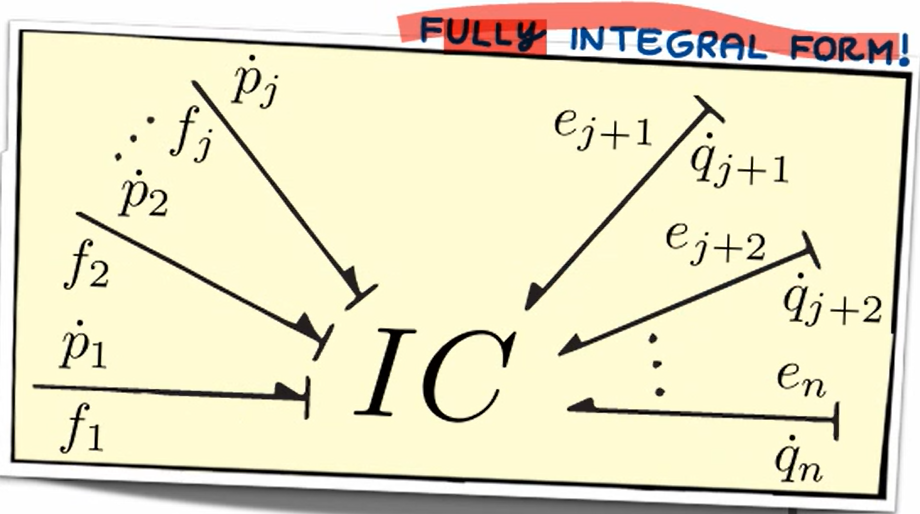
\includegraphics[scale=0.25]{figs/chapter5/5_7.png}
  \caption{IC-field with two I-ports and two C-ports}
\end{figure}

\begin{example}[Movable-Plate Capacitor]
A capacitor where one plate can move mechanically acts as a C-port electrically (charge $q$) and a C-port mechanically (position $x$). The stored energy is $E(q,x) = \frac{1}{2}\frac{q^2}{C(x)}$. The constitutive equations are:
\begin{equation}
    e = \frac{\partial E}{\partial q} = \frac{q}{C(x)} \qquad \text{and} \qquad F = \frac{\partial E}{\partial x} = -\frac{1}{2}\frac{q^2}{C^2(x)}\frac{\partial C}{\partial x}
\end{equation}

\begin{figure}[H]
  \centering
  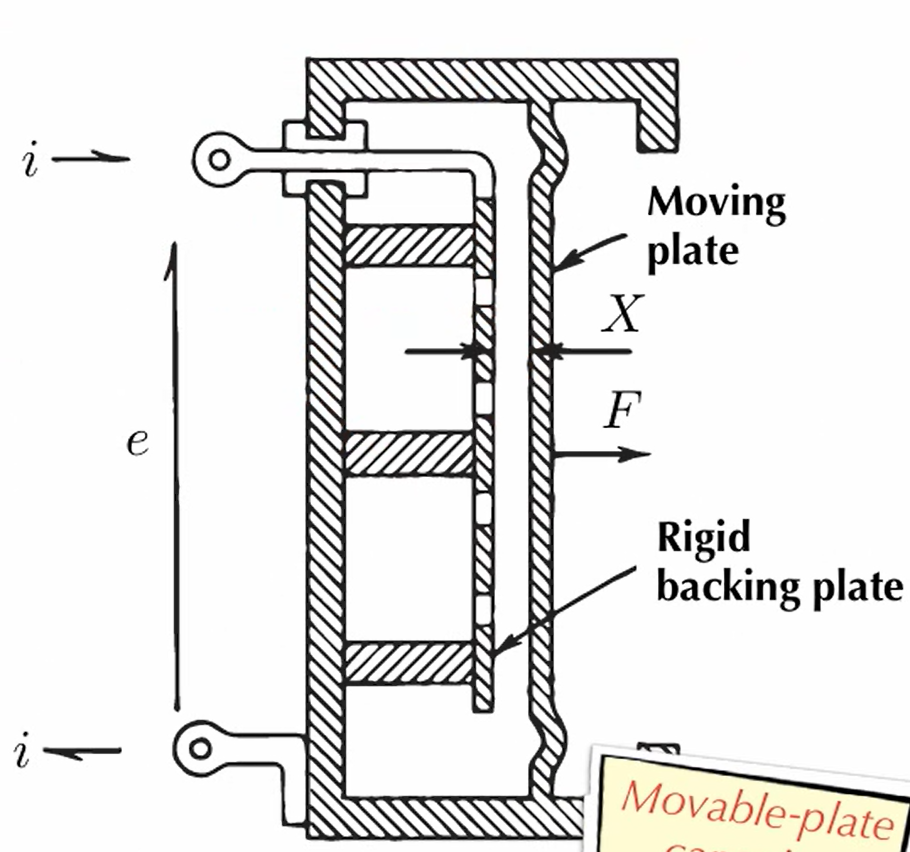
\includegraphics[scale=0.25]{figs/chapter5/5_8.png}
  \caption{Movable-plate capacitor as an IC-field}
\end{figure}

\end{example}




\begin{example}[Electrical Solenoid]
The electrical solenoid serves as a prototype of an IC-field transducer. From the electrical port, the coil exhibits self-inductance ($\lambda$). From the mechanical port, the force on the slug depends on its position ($x$). The energy is $E(\lambda,x) = \frac{1}{2}\frac{\lambda^2}{L(x)}$. The constitutive equations are:
\begin{equation}
    i = \frac{\partial E}{\partial \lambda} = \frac{\lambda}{L(x)} \qquad \text{and} \qquad F = \frac{\partial E}{\partial x} = -\frac{1}{2}\frac{\lambda^2}{L^2(x)}\frac{\partial L}{\partial x}
\end{equation}

\begin{figure}[H]
  \centering
  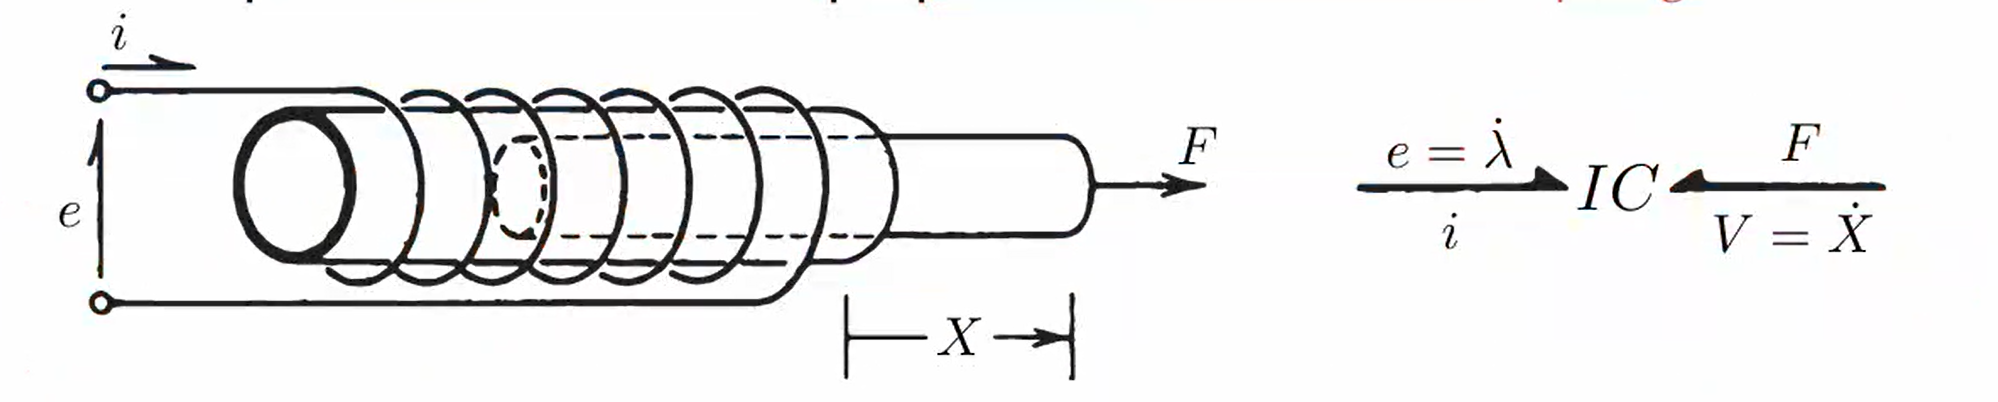
\includegraphics[scale=0.25]{figs/chapter5/5_9.png}
  \caption{Electrical solenoid as an IC-field}
\end{figure}

\end{example}


\section{R-fields: multiport dissipation}

An \textbf{R-field} is an $n$-port with a static (or algebraic) constitutive law that relates efforts and flows. In general, R-fields are \textbf{NOT} strictly related or associated to power losses: their TRUE intrinsic characteristic is to algebraically relate efforts and flows! 

This broad definition includes power-conserving elements, such as 0- and 1-junctions, and elements containing sources. However, in practice, most explicit R-fields do dissipate power (e.g. thermal resistors, coupled fluid friction matrices). Explicit R-fields arise frequently in modelling nonlinear devices.

The causality of an R-field is determined by the sources and energy-storing elements attached to it. 
\begin{itemize}
    \item \textbf{Resistance causality:} All flows are inputs, efforts are outputs ($e_i = \Phi_{R_i}(f_1 \dots f_n)$).
    \item \textbf{Conductance causality:} All efforts are inputs, flows are outputs ($f_i = \Phi_{R_i}^{-1}(e_1 \dots e_n)$).
    \item \textbf{Mixed causality:} A mixture of effort and flow inputs. 
\end{itemize}


\begin{figure}[H]
  \centering
  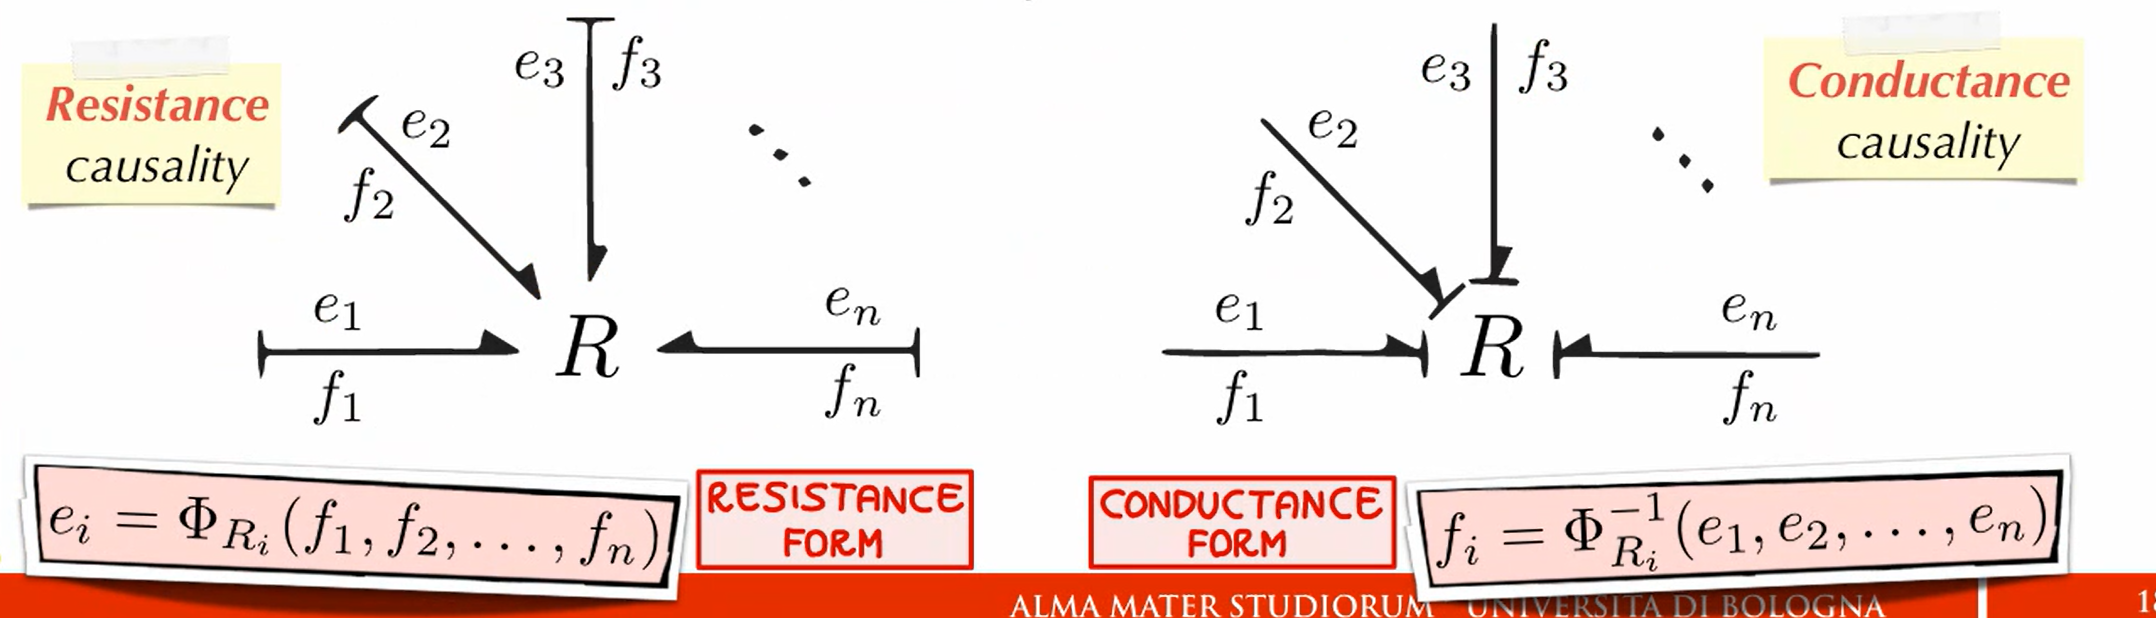
\includegraphics[scale=0.25]{figs/chapter5/5_10.png}
  \caption{Causality in R-fields}
\end{figure}

\paragraph{Onsager vs. Casimir Forms and Power.}
Since an R-field has no stored energy function, there is no direct equivalent to Maxwell's Reciprocal Relations. However, structural properties do exist. Any square Constitutive Law Matrix (CLM) $M$ can always be mathematically decomposed into a symmetric part $M_S = \frac{1}{2}(M+M^T)$ and a skew-symmetric (antisymmetric) part $M_A = \frac{1}{2}(M-M^T)$. 

The asymmetric contribution $M_A$ is always related to \emph{perfectly conserved power} ($P_w = b^T M_A b = 0$). The symmetric part $M_S$ is associated with power dissipation.

Implicit R-fields composed strictly of linear 1-port resistances, 0-junctions, 1-junctions, and transformers will obey \textbf{Onsager Reciprocity}: when expressed in pure resistance or conductance form, their CLM is perfectly symmetric (called the \emph{Onsager form}). When expressed in mixed causality, the matrix is guaranteed to present asymmetric terms. 

Importantly, NOT all R-fields obey Onsager Reciprocity. If Gyrators (GY) are allowed inside the implicit R-field, the reciprocity is broken, yielding asymmetric terms even in pure resistance/conductance forms. This is known as the \textbf{Casimir form}.

There could be examples of R-fields that are not Onsager and Casimir at the same time, but a mix of the two. 

\begin{figure} [H]
  \centering
  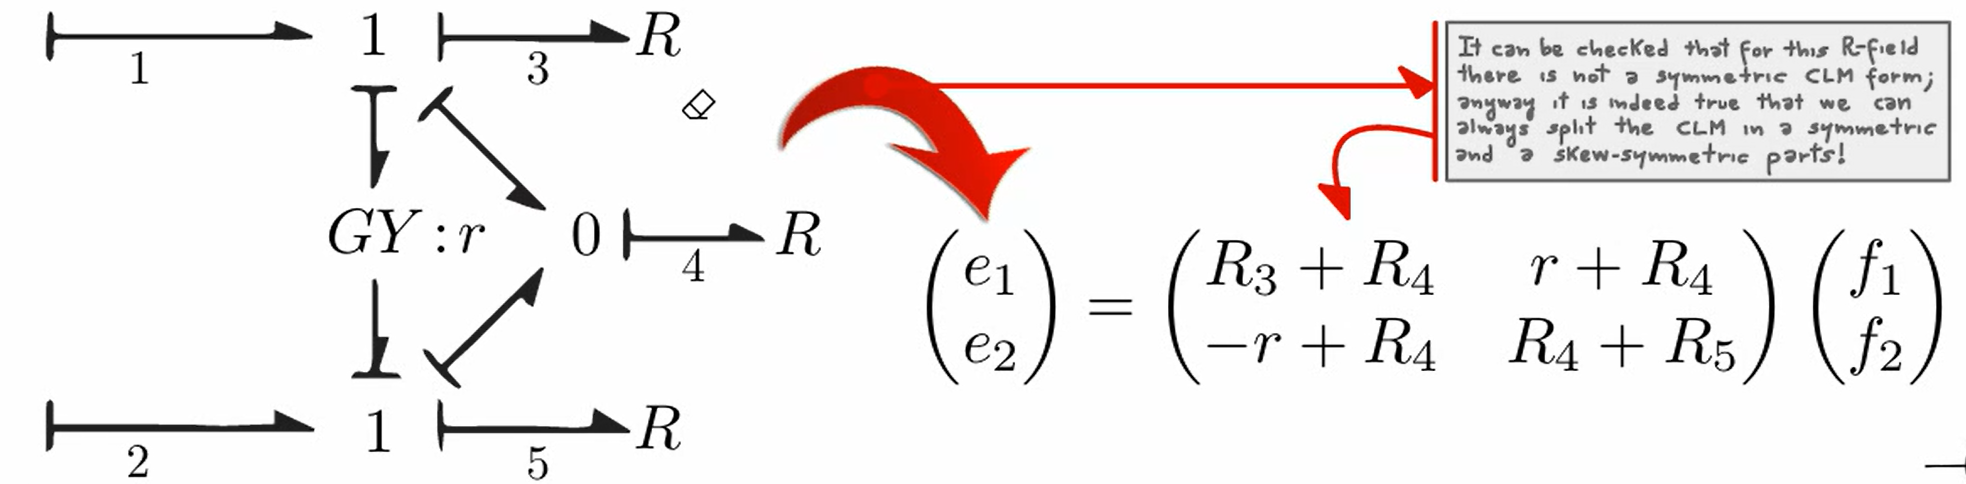
\includegraphics[scale=0.25]{figs/chapter5/5_11.png}
  \caption{R-field without Onsager and Casimir reciprocity}
\end{figure}


\section{Modulated 2-port elements}

Before discussing pure junction structures, it is essential to introduce the modulated 2-ports. The \textbf{modulated transformer (MTF)} and \textbf{modulated gyrator (MGY)} are nonlinear, power-conserving generalisations of TF and GY. 

The parameters (modulus $m$ or $r$) of these elements are allowed to be a function of some other parameter in the system (often a displacement or angle, possibly time-varying). These parameters are modulated by means of a signal (active bond) rather than a power bond. Thus, it is characteristic of these elements that the parameters change value without a directly associated power flow!

Examples include the DC motor (Faraday \& Lorentz laws modelled as an MGY depending on field current) and the slider-crank or rack-and-pinion mechanisms (modelled as MTF). 


\section{Junction structures}

\textbf{Junction structures} are the energy switchyards that enforce the constraints among parts of dynamic systems. They result from the interconnection of 0-junctions, 1-junctions, TF, and GY. They contain no dissipative or storage elements.

Junction structures are essentially special types of R-fields that \emph{never} dissipate power (meaning their CLM is completely skew-symmetric). They are always \textbf{anti-symmetric} because they cannot dissipate power. Because they cannot dissipate power, they typically \textbf{cannot} accept all possible causal assignments at their ports (e.g., a pure junction structure without gyrators cannot accept resistance or conductance causality on all ports simultaneously).

Junction structures have a key property: they are themselves power-conserving, so $\sum_k e_k f_k = 0$ across all their external ports. Equivalently, the junction structure defines a set of linear constraints (from the junctions) and scaling/exchange rules (from TF and GY) on the port variables.

\begin{figure}[H]
  \centering
  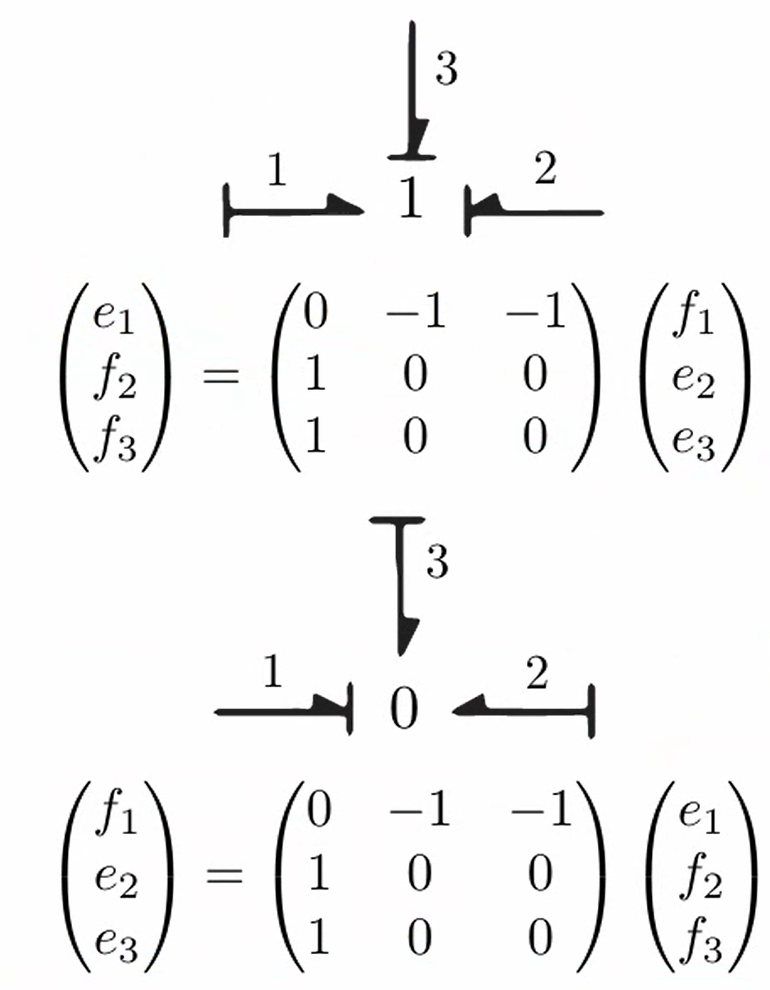
\includegraphics[scale=0.25]{figs/chapter5/5_12.png}
  \caption{Junction structure as a power-conserving R-field}
\end{figure}


\subsection{Multiport Transformers (Kinematics)}

Another extremely interesting viewpoint about junction structures involves the transformations of variables they provide. A \textbf{multiport transformer} is a specific assemblage of 0s, 1s, and TFs that shows more than two ports to the external world. 

Mathematically, a multiport transformer is characterised by a matrix $\mathbf{G}$ and its transpose $\mathbf{G}^T$, just as a 2-port transformer is characterised by a single modulus $m$. By setting a "through" power convention (power in for inputs, out for outputs), the constitutive law can always be written as:

\begin{equation}
    \mathbf{e}_{in} = \mathbf{G} \cdot \mathbf{e}_{out} \qquad \text{and} \qquad \mathbf{f}_{out} = \mathbf{G}^T \cdot \mathbf{f}_{in}
\end{equation}

\begin{figure}[H]
  \centering
  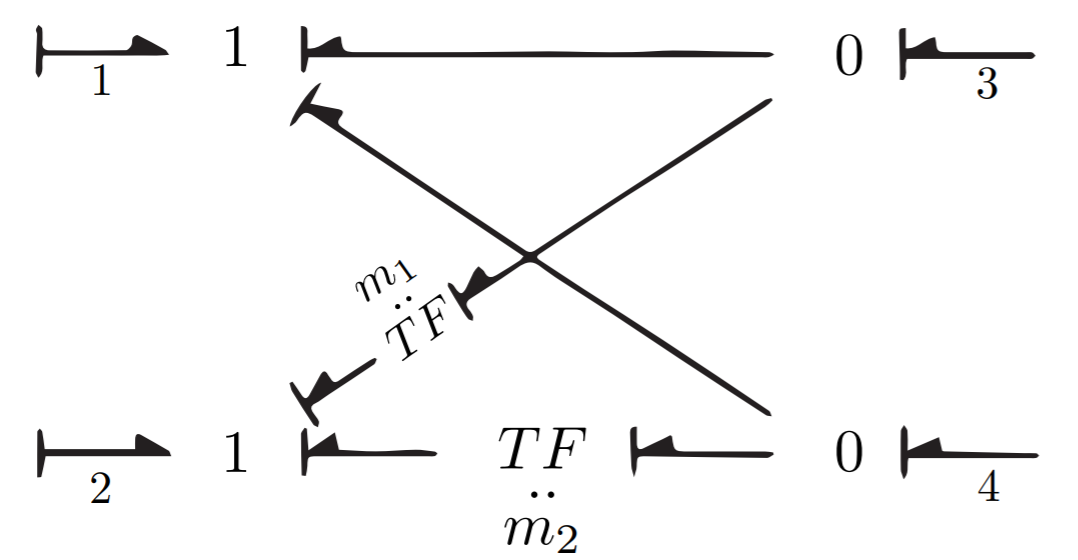
\includegraphics[scale=0.25]{figs/chapter5/5_13.png}
  \caption{Multiport transformer as a power-conserving R-field}
\end{figure}


This is exactly the formulation used for 3D Kinematics and coordinate transformations! A typical example is implementing a Jacobian $J(q)$ that links a joint-coordinate space to a Cartesian-coordinate space in robotics. The forward kinematics ($\dot{x} = J(q)\dot{q}$) dictates the flow transformations, and by power conservation, the transpose Jacobian dictates the force-torque effort transformations ($T = J^T(q)F$). Grouping these into a multiport MTF field elegantly handles 3D kinematics directly within the bond graph framework.



%──────────────────────────────────────────────────────────────────────
\part{Mechanical, Distributed and Thermo-fluid Systems}
%──────────────────────────────────────────────────────────────────────
 %%%%%%%%%%%%%%%%%%%%%%%%%%%%%%%%%%%%%%%%%%%%%%%%%%%%%%%%%%%%%%%%%%%%%%%
\chapter{Multi-body Systems}
\label{ch:multibody}
%%%%%%%%%%%%%%%%%%%%%%%%%%%%%%%%%%%%%%%%%%%%%%%%%%%%%%%%%%%%%%%%%%%%%%%



Extending bond graph modelling from 2D plane motion to full \textbf{3D rigid-body mechanics} brings geometric nonlinearity through the rotation group. These geometric nonlinearities are a primary cause of equation formulation problems. The key modelling choice — whether to express quantities in the inertial frame or a body-fixed frame — has direct consequences for the structure of the equations and the bond graph.

\section{Dynamics of a 3D rigid body}

Consider a rigid body of mass $m$ with moments of inertia $J_x, J_y, J_z$ along the principal axes. The body-fixed coordinate frame $\{G; x, y, z\}$ is attached to the center of mass $G$ with axes aligned with the principal axes of inertia. 

\paragraph{Why the body frame?}
In the inertial frame, the inertia tensor $\mathbf{J}$ is a $3\times3$ matrix that varies with the body's orientation — making the constitutive equations of the I-field time-varying and complex. In the body frame, $\mathbf{J} = \mathrm{diag}(J_x, J_y, J_z)$ is \textbf{constant}, which is the primary advantage of this formulation. The mass $m$ and inertia $\mathbf{J}$ are invariant, making them highly practical coordinates for computation.

The price is that Newton's law in the body frame contains \textbf{nonlinear gyroscopic terms} from the frame's own rotation. Newton's law applied in the body frame requires accounting for the rate of change of momentum relative to the moving frame.

\paragraph{Newton--Euler equations.}
Let $\mathbf{v} = (v_x, v_y, v_z)^T$ and $\boldsymbol{\omega} = (\omega_x, \omega_y, \omega_z)^T$ be the translational velocity of $G$ and the angular velocity, \emph{both expressed in the body frame}. Let $\mathbf{F}$ and $\boldsymbol{\tau}$ be force and torque at $G$ in the body frame. Then:
\begin{equation}
  \mathbf{F} = \dot{\mathbf{p}} + \boldsymbol{\omega}\times\mathbf{p},
  \qquad \mathbf{p} = m\mathbf{v},
\end{equation}
\begin{equation}
  \boldsymbol{\tau} = \dot{\mathbf{h}} + \boldsymbol{\omega}\times\mathbf{h},
  \qquad \mathbf{h} = \mathbf{J}\boldsymbol{\omega}.
\end{equation}
Written component-wise, these are the \textbf{Euler equations}:
\begin{align}
  F_x &= m\dot{v}_x + m\omega_y v_z - m\omega_z v_y \notag\\
  F_y &= m\dot{v}_y + m\omega_z v_x - m\omega_x v_z \notag\\
  F_z &= m\dot{v}_z + m\omega_x v_y - m\omega_y v_x \notag\\[4pt]
  \tau_x &= J_x\dot{\omega}_x + \omega_y J_z\omega_z - \omega_z J_y\omega_y \notag\\
  \tau_y &= J_y\dot{\omega}_y + \omega_z J_x\omega_x - \omega_x J_z\omega_z \notag\\
  \tau_z &= J_z\dot{\omega}_z + \omega_x J_y\omega_y - \omega_y J_x\omega_x.
\end{align}


\begin{insightbox}
  Note that we are dealing the body fixed frame here. This is just the derivative wrt to time of a vector, that in this case are the momentum ($p$) and the angular momentum ($h$). There is a \textbf{hidden frame fixed to the momentum vectors.} 

  The angular momentum formula is more intuitive since it's more used as we work with fixed body frame with fixed inertia and axis of inertia. This is not usually done with forces, since we see them in the inertial frame. 

  Note also that it's always possible to measure $\omega$ with a gyro, since all the points in a rigid body have the same angular velocity. However, the linear velocity of the CoG is not directly measurable by a sensor fixed to the body, since it depends on the point itself. That's why we don't use the first equations in practice.

  \begin{figure} [H]
    \centering
    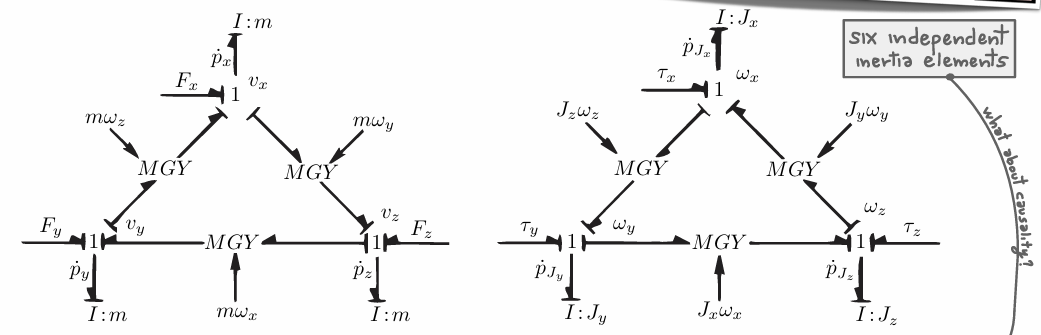
\includegraphics[width=0.8\textwidth]{figs/chapter6/6_1.png}
    \caption{Considerations on the body frame and the hidden frame of the momentum vectors.}
  \end{figure}

\end{insightbox}



These nonlinear differential equations have no general analytical solution. Furthermore, they provide velocities with respect to a frame that is aiming in a different direction at every instant. The cross-product terms $\boldsymbol{\omega}\times\mathbf{p}$ and $\boldsymbol{\omega}\times\mathbf{h}$ are gyroscopic: they do not do work (they are perpendicular to velocity), but they redistribute momentum between components. In the bond graph, they appear as \textbf{modulated gyrators} (MGY elements) whose moduli depend on the angular velocity — making the model intrinsically nonlinear.

\begin{insightbox}[The I-field of a 3D rigid body vs. Independent Elements]
The 3D rigid body is conceptually represented by a \textbf{6-port I-field} in the body frame: three translational ports and three rotational ports. The constitutive law (flow = $\mathbf{M}^{-1}\mathbf{p}$, with block-diagonal $\mathbf{M} = \mathrm{diag}(m\mathbf{I}_3, \mathbf{J})$) is linear and constant. 

However, \emph{attention must be paid to the actual bond graph implementation}. In practice, this block is modelled as \textbf{six independent 1-port I-elements}, which are in integral causality. (since the mass matrix is diagonal in the principal body frame), interconnected by an Eulerian junction structure containing the MGYs. The nonlinear gyroscopic interaction is handled by MGY elements in the junction structure, not inside the I-elements themselves. This separation of linear storage from nonlinear routing is elegant and computationally efficient. As long as external forces and torques are causal inputs, integral causality exists for all six I-elements.
\end{insightbox}

\begin{figure} [H]
  \centering
  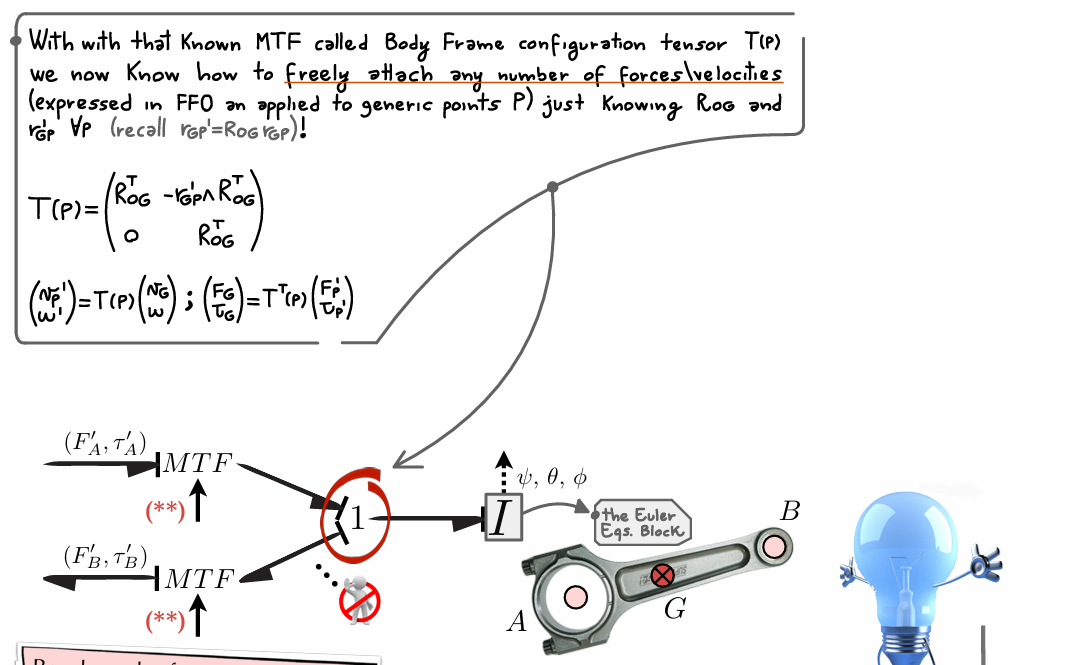
\includegraphics[width=0.8\textwidth]{figs/chapter6/6_2.png}
  \caption{The I-field of a 3D rigid body is often implemented as six independent I-elements (three for translation, three for rotation) interconnected by a junction structure that encodes the gyroscopic interactions via MGY elements.}   
\end{figure}

\begin{figure}
  \centering
  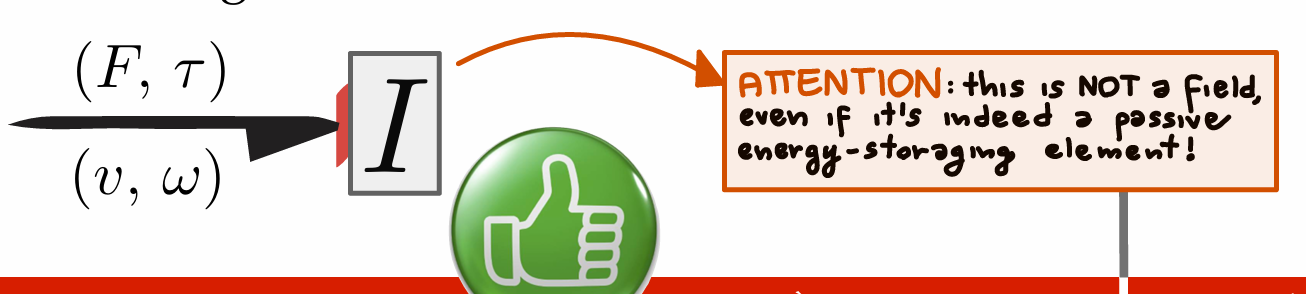
\includegraphics[width=0.8\textwidth]{figs/chapter6/6_2_1.png}
  \caption{THis is not a single field, this is a double field because they are two separated systems.}
\end{figure}

Note that in the bond enters the ($F_x, _y, F_z$) forces that's important to mention that they are refered to the body frame (which is moving w.r.t. the inertial frame). Forces assign causality effort, and the I-field is in integral causality, so the velocities are outputs. The MGY elements take these velocities and feed them back into the I-field to account for the gyroscopic effects.

\section{Rotation matrices and coordinate transformations}

Since all velocities and forces are expressed in the body frame, but external loads and gravity often come from the inertial frame (where e.g., gravity acts strictly downwards), coordinate transformations are necessary. We need an appropriate "junction element" to bridge the body frame and the inertial frame.

The rotation matrix $\mathbf{R}(t)$ (a $3\times3$ orthogonal matrix with $\mathbf{R}^T\mathbf{R} = \mathbf{I}$, $\det\mathbf{R} = 1$) transforms vectors from the body frame to the inertial frame ($\mathbf{w}_{inertial} = \mathbf{R} \mathbf{w}_{body}$). In bond graphs, $\mathbf{R}$ acts as a Modulated Transformer (MTF) that conserves power.

\paragraph{Yaw, Pitch, and Roll (Cardan Angles).}
Any spatial transformation consists of a series of coordinate rotations. For spinning bodies, Euler angles are typical, but for multi-body systems like robotic arms or aircraft, Yaw ($\psi$), Pitch ($\theta$), and Roll ($\phi$) (Cardan Angles) are frequently used. The combined rotation matrix is $\mathbf{R}_{\psi\theta\phi} = \mathbf{R}_\psi \mathbf{R}_\theta \mathbf{R}_\phi$.

By mapping the body-frame angular velocity $\boldsymbol{\omega}$ to the angle derivatives, we obtain the kinematic relationships:
\begin{align}
  \dot{\psi} &= \frac{\sin\phi}{\cos\theta}\omega_y + \frac{\cos\phi}{\cos\theta}\omega_z \\
  \dot{\theta} &= \cos\phi\, \omega_y - \sin\phi\, \omega_z \\
  \dot{\phi} &= \omega_x + \sin\phi\frac{\sin\theta}{\cos\theta}\omega_y + \cos\phi\frac{\sin\theta}{\cos\theta}\omega_z
\end{align}

\begin{figure} [H]
  \centering
  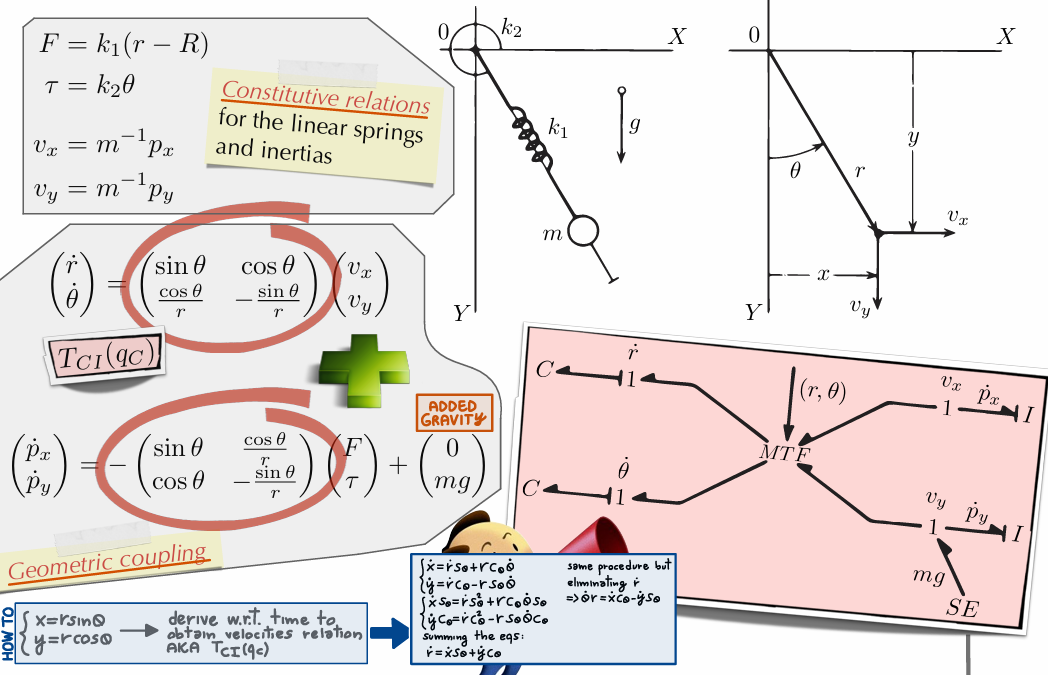
\includegraphics[width=0.8\textwidth]{figs/chapter6/6_3.png}
  \caption{Roll pitch and yaw rotation matrices}  
\end{figure}


Care must be taken regarding kinematic singularities (e.g., when $\cos\theta = 0$). Alternatively, one can directly integrate the differential equation of the rotation matrix:
\begin{equation}
  \dot{\mathbf{R}} = \mathbf{R}\,\mathbf{S}(\boldsymbol{\omega})
\end{equation}
where $\mathbf{S}(\boldsymbol{\omega})$ is the skew-symmetric matrix:
\begin{equation}
  \mathbf{S}(\boldsymbol{\omega}) = \begin{pmatrix}0 & -\omega_z & \omega_y\\\omega_z & 0 & -\omega_x\\-\omega_y & \omega_x & 0\end{pmatrix}.
\end{equation}
The quantity $\dot{\mathbf{R}}\mathbf{R}^T = \mathbf{R}\,\mathbf{S}(\boldsymbol{\omega})\,\mathbf{R}^T$ is the angular velocity in the inertial frame expressed as a skew-symmetric matrix. In the bond graph, MTF elements with moduli from $\mathbf{R}$ handle these transformations when coupling to the environment or to other bodies.

\begin{figure} [H]
  \centering
  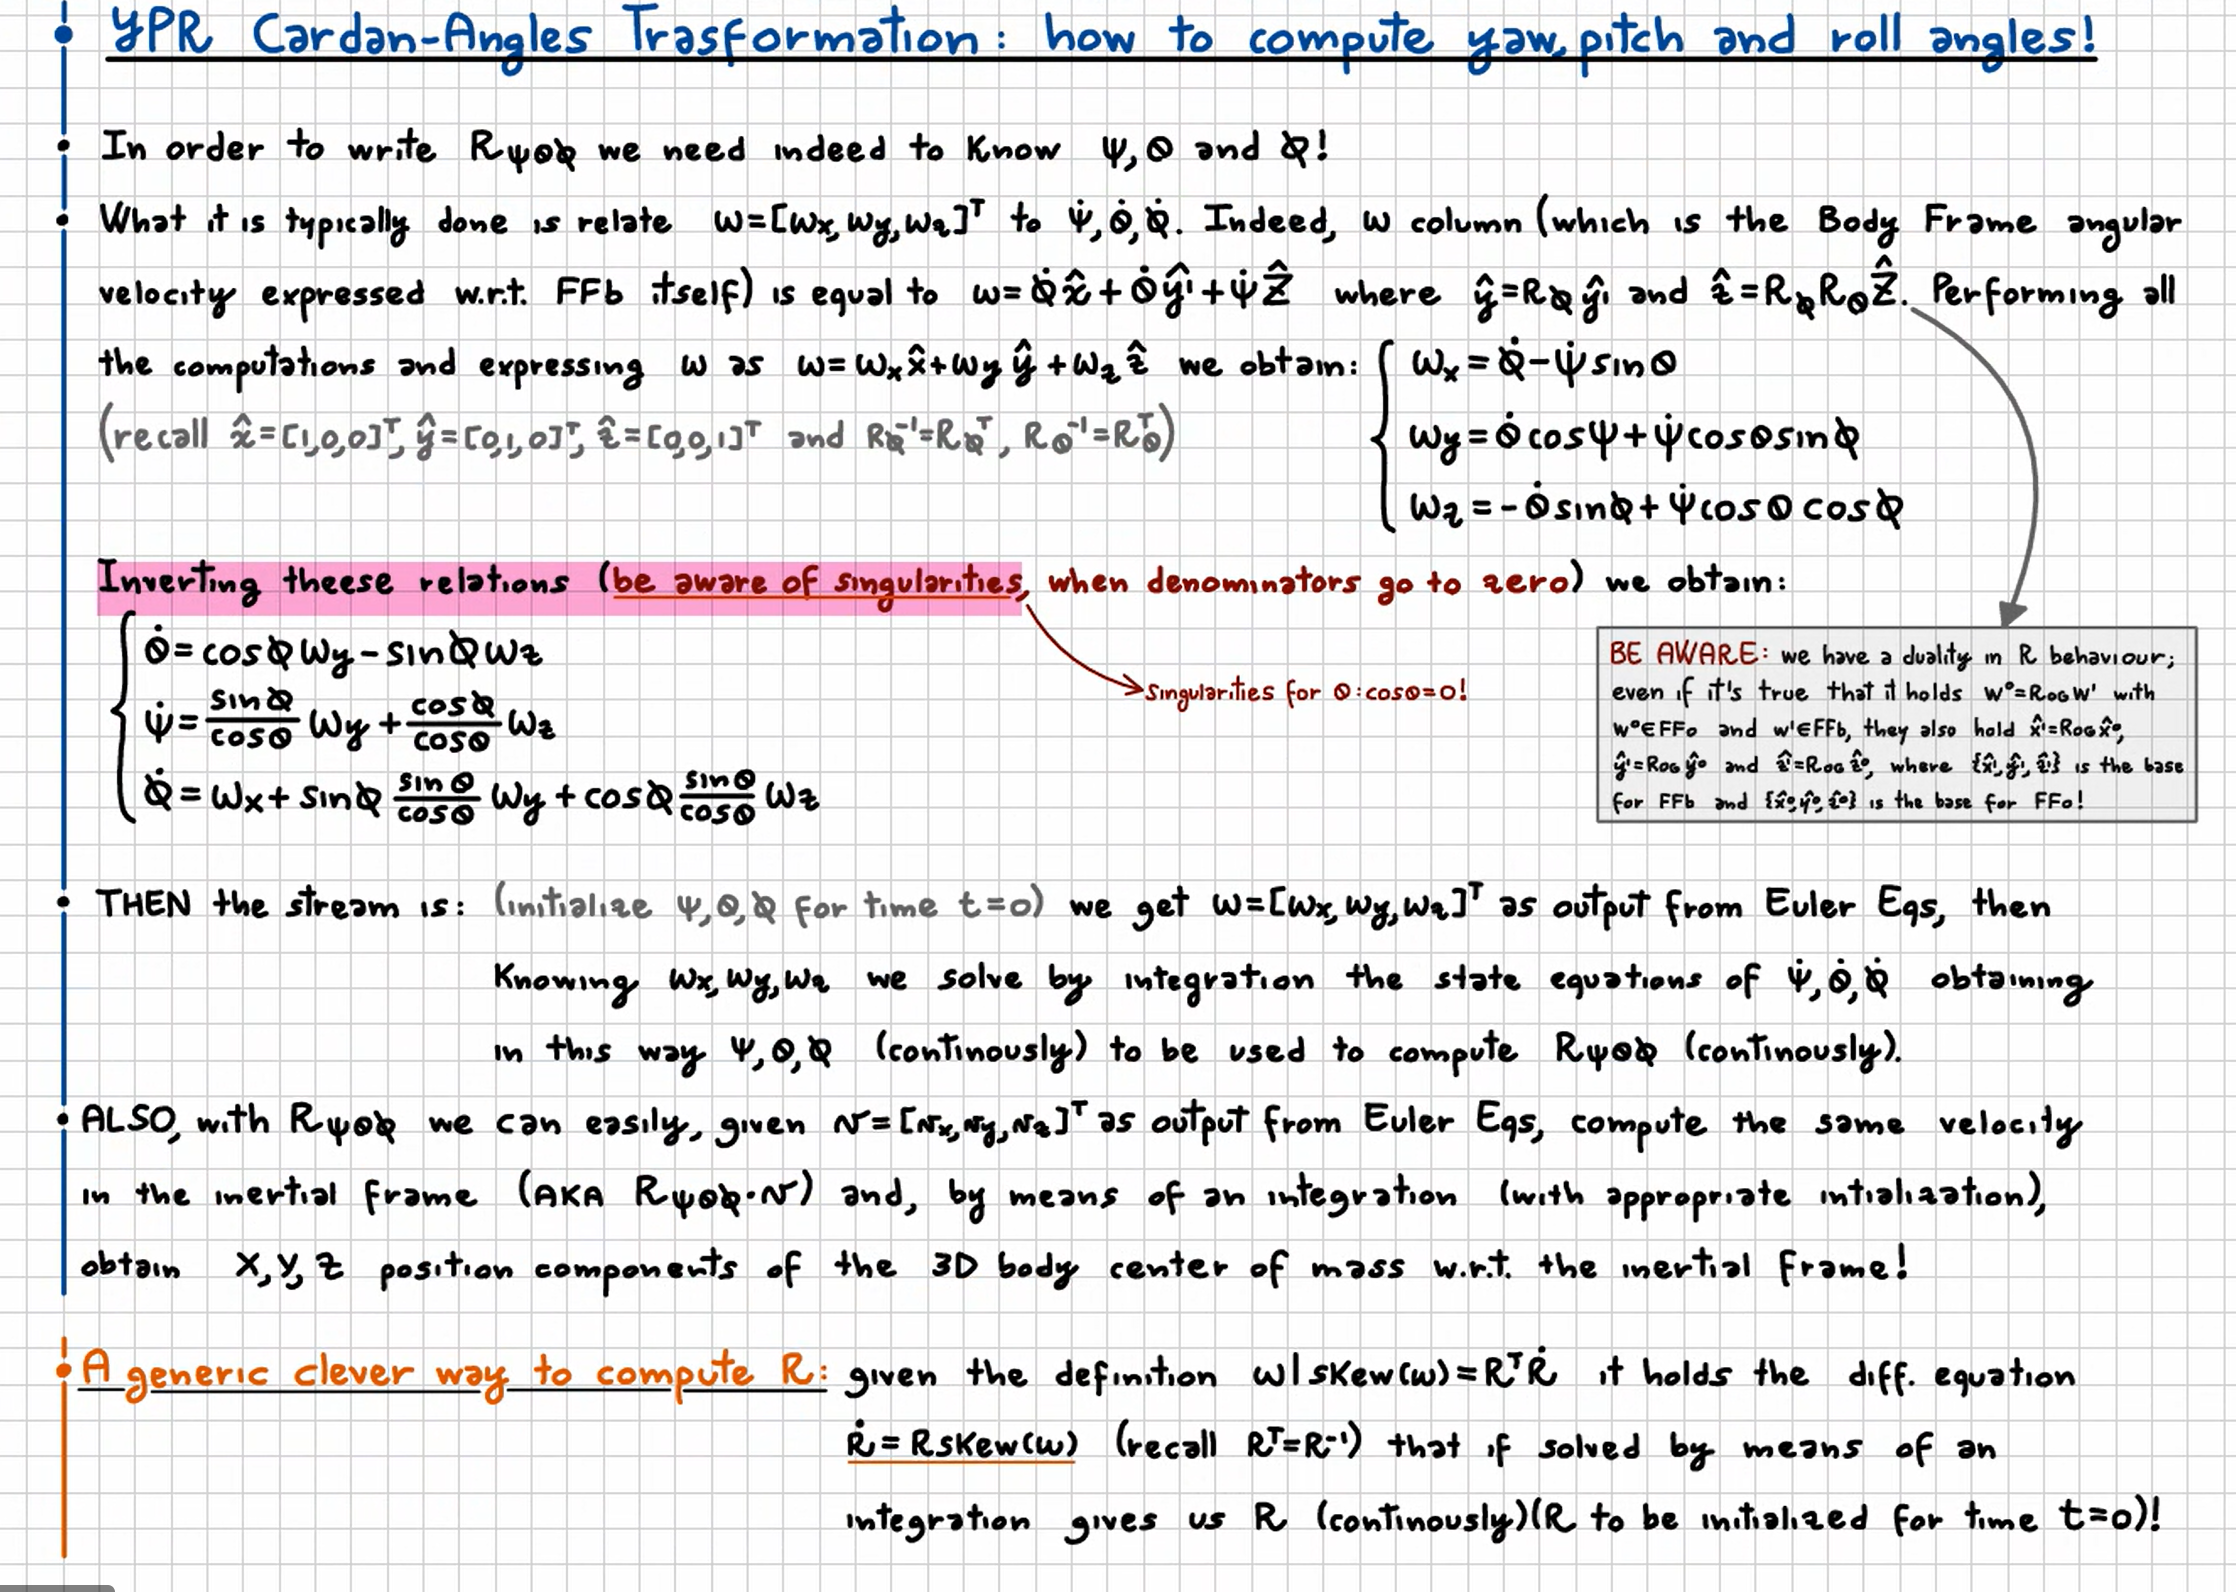
\includegraphics[width=0.8\textwidth]{figs/chapter6/6_4.png}
  \caption{Andrea Lombardi insight}
\end{figure}


\paragraph{Multidimensional dynamics}

We can always tranform the body-fixed variables into inertial frame variables by using a modulated transformer that handles the rotation. 

\begin{figure}[H]
  \centering
  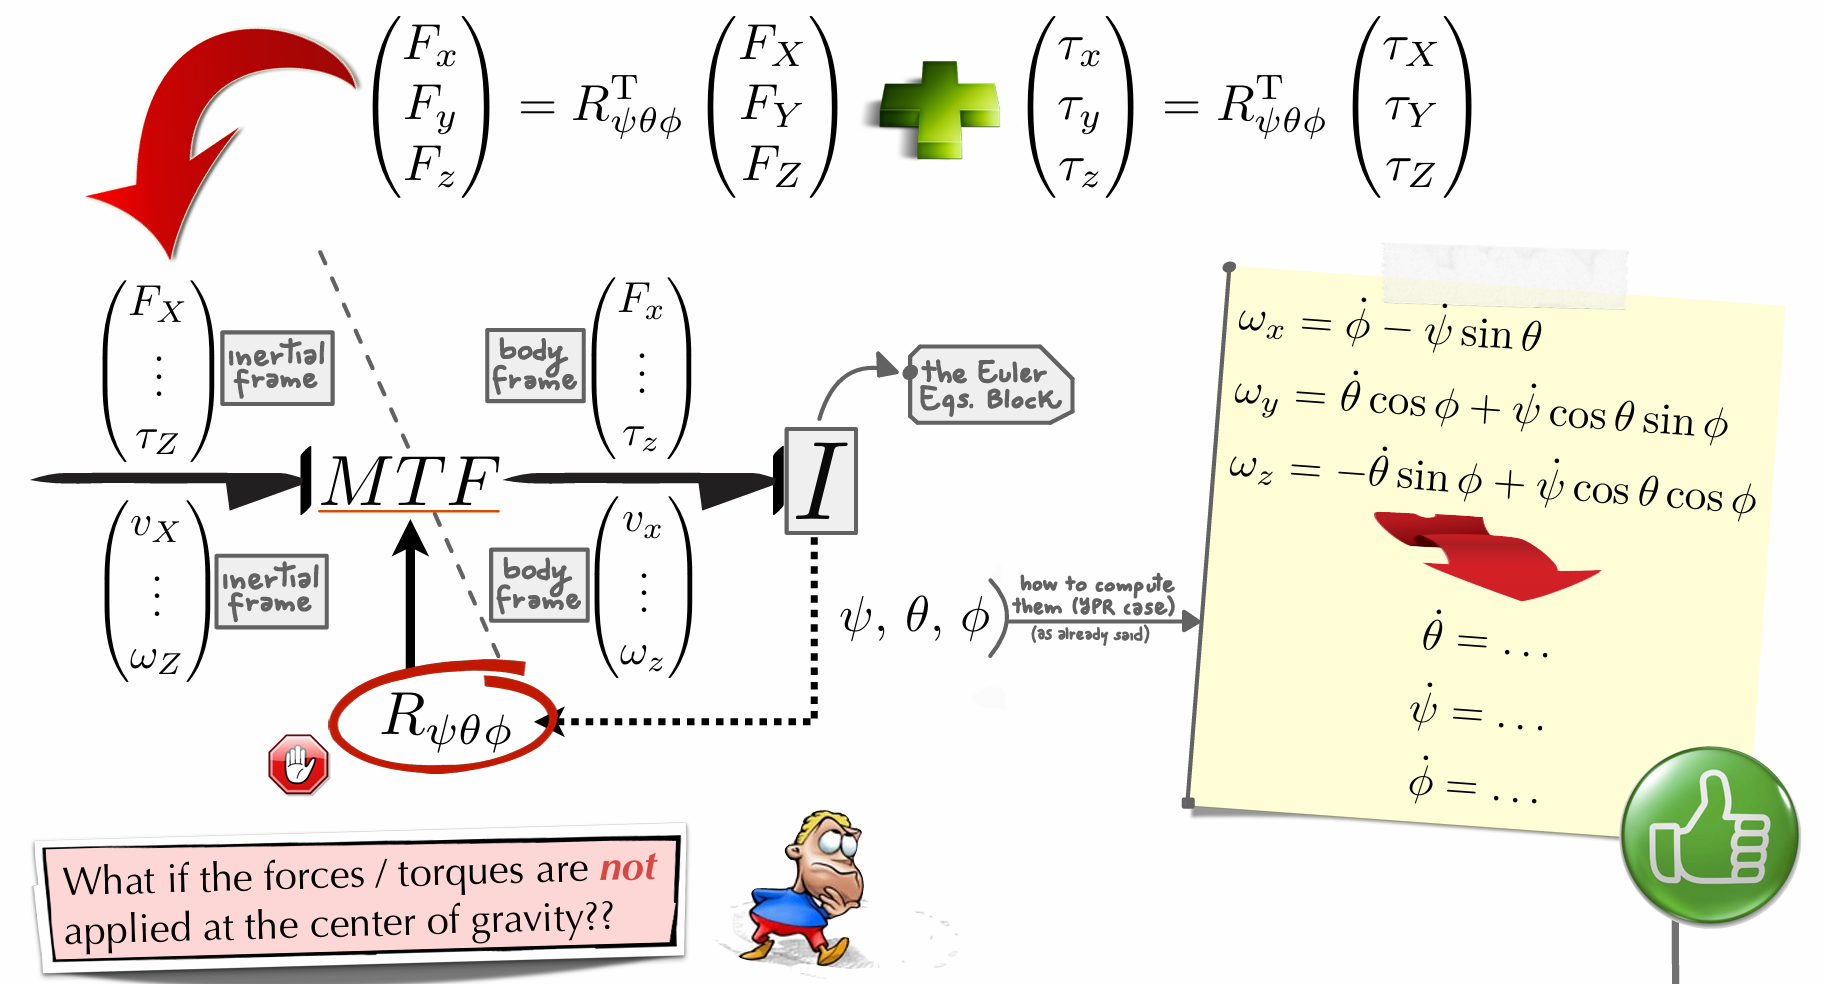
\includegraphics[width=0.8\textwidth]{figs/chapter6/6_5.png}
  \caption{The rotation matrix $\mathbf{R}$ acts as a modulated transformer (MTF) that converts body-frame velocities and forces to inertial-frame quantities, allowing us to connect the rigid body I-field to external forces and gravity defined in the inertial frame.}
\end{figure}


\paragraph{Forces not applied at the Centre of Gravity.}
Often, connecting forces are applied at a point $P$ offset from the CoG $G$ by a fixed vector $\mathbf{r}_{GP}$ in the body frame. The velocity of point $P$ is given by:
\begin{equation}
  \mathbf{v}_P = \mathbf{v}_G + \boldsymbol{\omega} \times \mathbf{r}_{GP}
\end{equation}
In matrix form, this kinematic relationship defines a \textbf{Body Frame Configuration Tensor} $\mathbf{T}(P)$:
\begin{equation}
  \begin{pmatrix}\mathbf{v}_P \\ \boldsymbol{\omega}\end{pmatrix} = \begin{pmatrix}\mathbf{I} & -\mathbf{r}_{GP}\times \\ \mathbf{0} & \mathbf{I}\end{pmatrix} \begin{pmatrix}\mathbf{v}_G \\ \boldsymbol{\omega}\end{pmatrix}
\end{equation}
By power conservation, the transposed tensor maps the forces applied at $P$ back to equivalent forces and torques at the CoG:
\begin{equation}
  \begin{pmatrix}\mathbf{F}_G \\ \boldsymbol{\tau}_G\end{pmatrix} = \begin{pmatrix}\mathbf{I} & \mathbf{0} \\ \mathbf{r}_{GP}\times & \mathbf{I}\end{pmatrix} \begin{pmatrix}\mathbf{F}_P \\ \boldsymbol{\tau}_P\end{pmatrix}
\end{equation}
This allows us to freely attach any number of forces or velocities applied at generic points using an MTF block.

\begin{figure}[H]
  \centering
  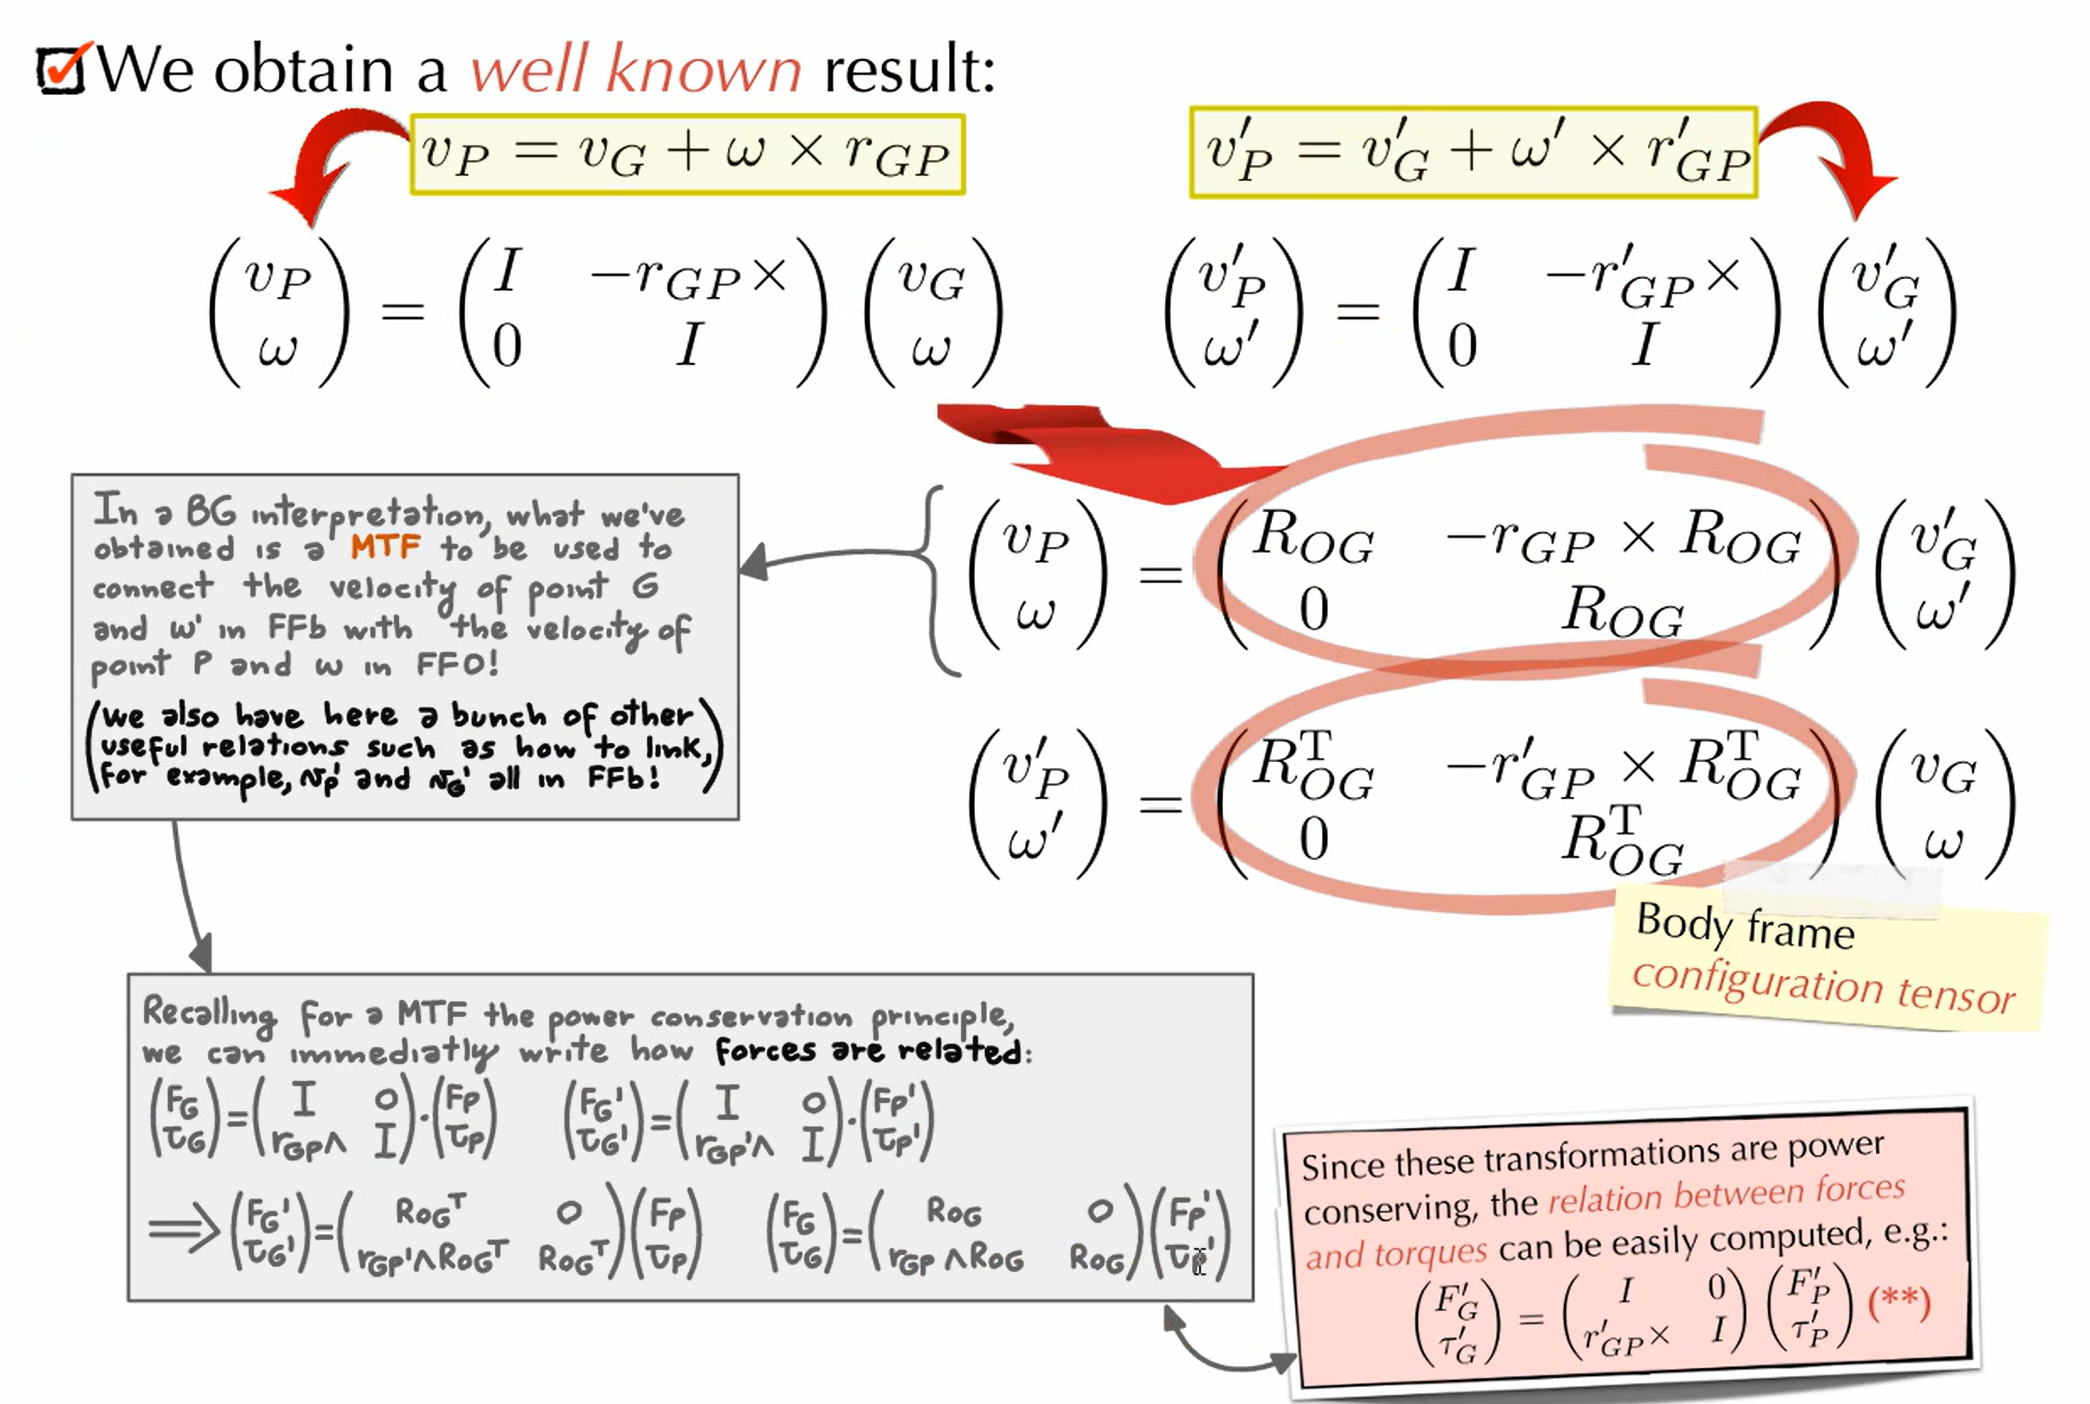
\includegraphics[width=0.8\textwidth]{figs/chapter6/6_6.png}
  \caption{Forces applied at a point $P$ offset from the CoG $G$ can be transformed to equivalent forces and torques at $G$ using a Body Frame Configuration Tensor $\mathbf{T}(P)$, which accounts for the lever arm effect of the offset.}
\end{figure}

We can write the whole rigid link bond graph in this manner: 

\begin{figure}[H]
  \centering
  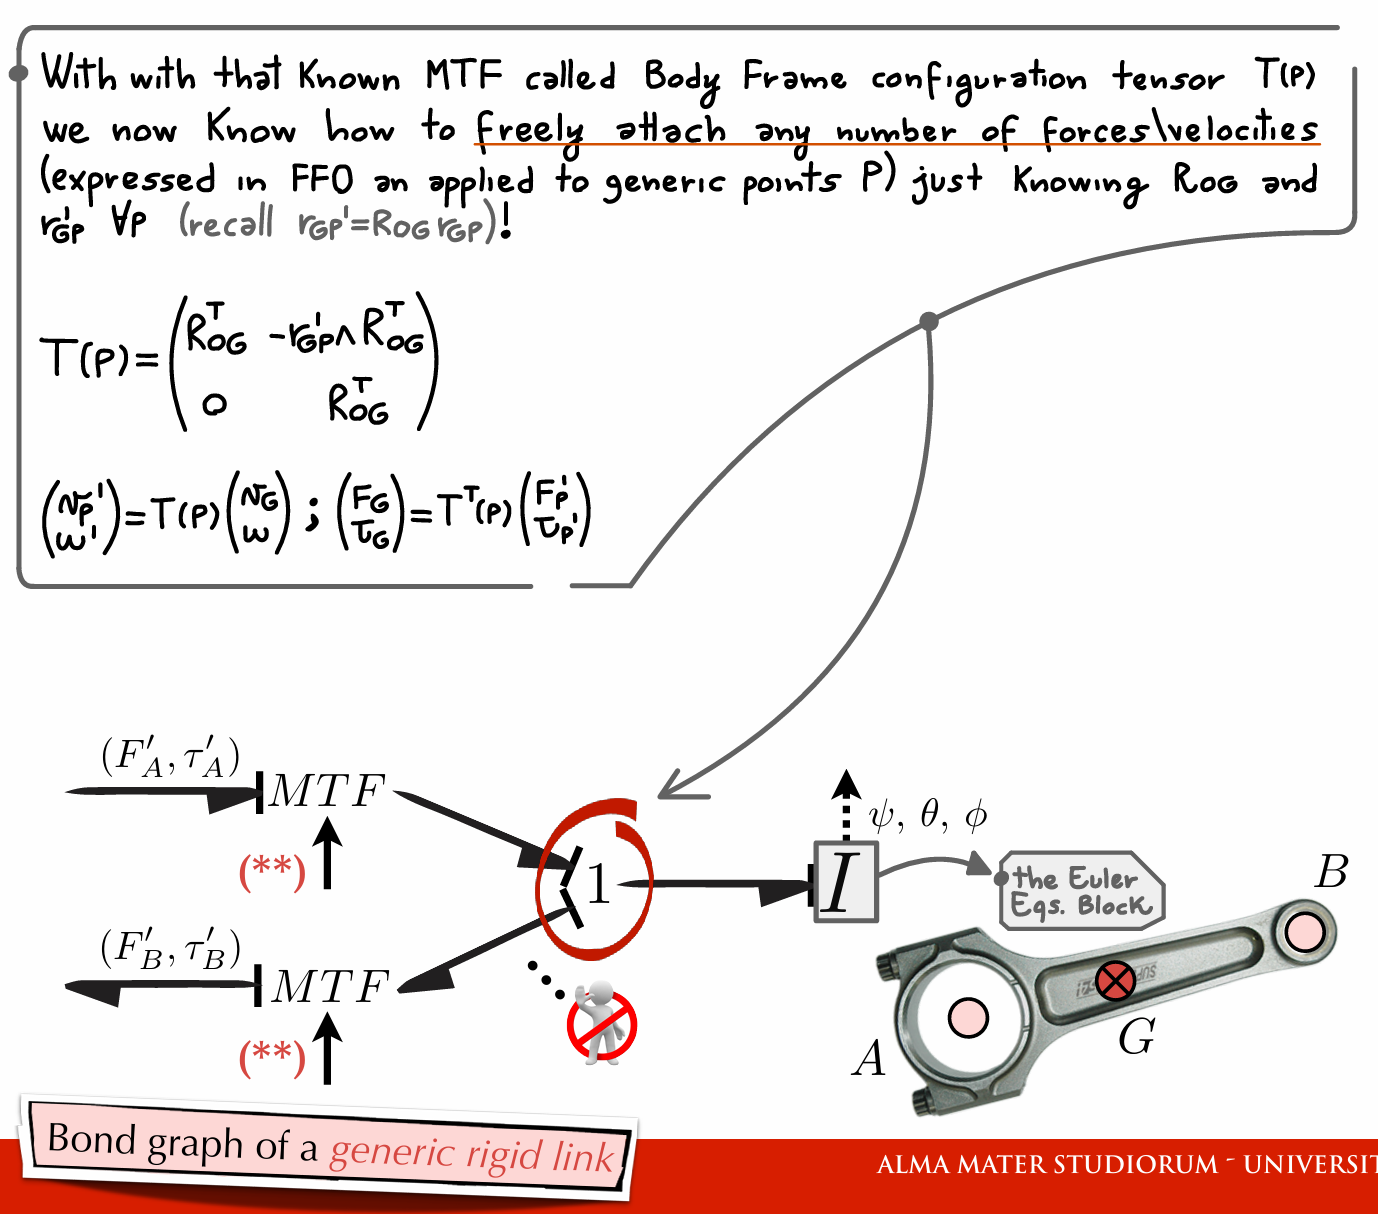
\includegraphics[width=0.8\textwidth]{figs/chapter6/6_7.png}
  \caption{The bond graph of a single rigid body in the inertial frame.}
\end{figure}

They are used to move from a point $A$ in the rigid body to a point $B$ in the same rigid body.

\section{Joints between rigid links}

A \textbf{joint} connects two rigid links by constraining their relative motion to a subspace. In the inertial frame:

\paragraph{Rotational (Revolute) joint.}
The relative linear velocity between the two attachment points is zero; the relative angular velocity $\omega_r = \omega_B - \omega_A$ is free (the joint can rotate). A torque $\tau_r$ acts along the joint axis. 
A revolute joint fully constrains linear velocities at the joint centre $P$, which is fixed with respect to both body frames. The bond graph imposes the velocity constraint via an MTF ($\mathbf{v}_P^A = \mathbf{R}_B^A \mathbf{v}_P^B$), and identifies the relative angular velocity:
\begin{equation}
  \mathbf{v}_A = \mathbf{v}_B \quad (\text{at the joint location}), \qquad
  \boldsymbol{\omega}_{AB}^A = \boldsymbol{\omega}_B^A - \boldsymbol{\omega}_A^A \text{ (free)}.
\end{equation}

\begin{figure}[H]
  \centering
  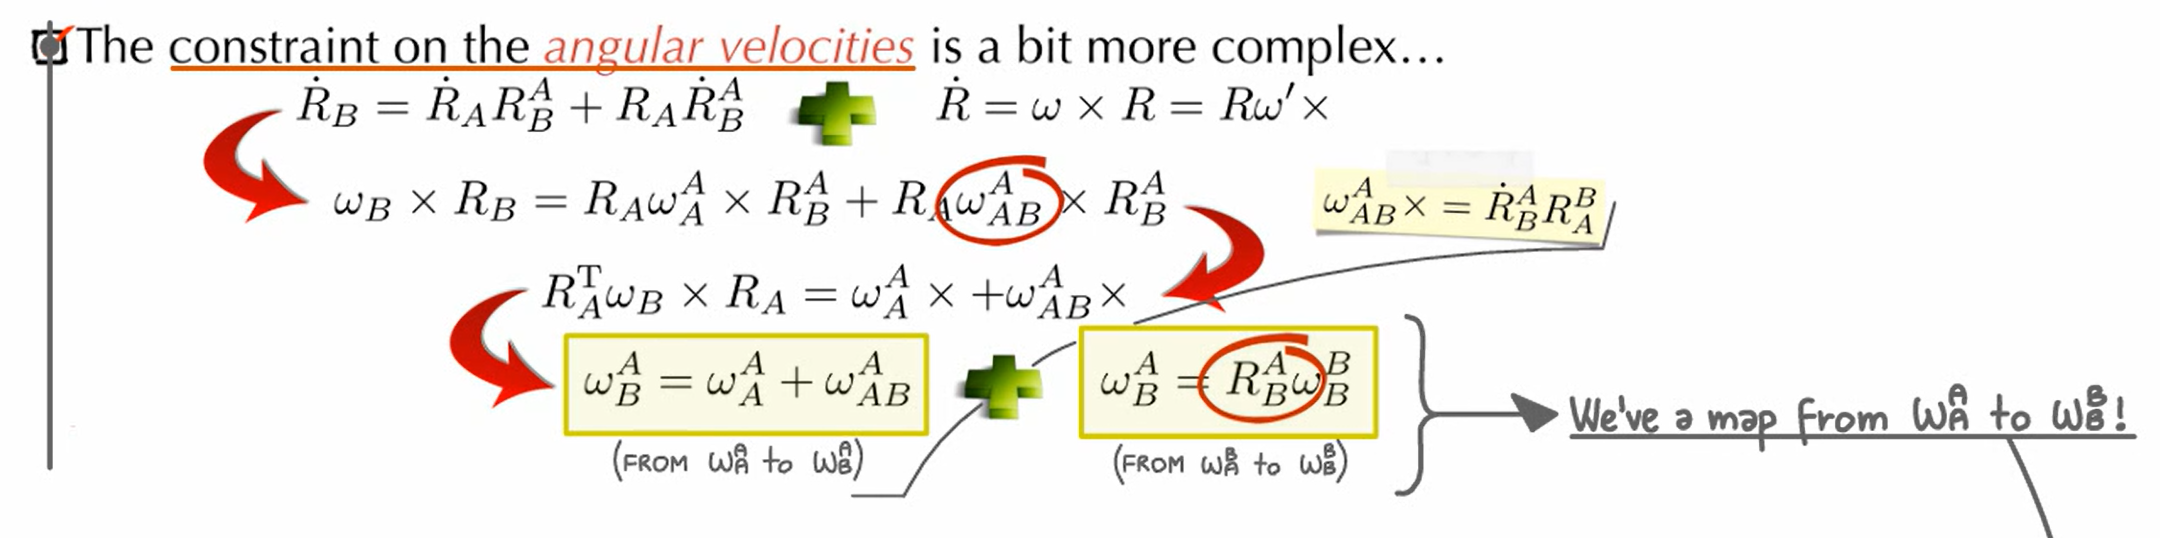
\includegraphics[width=0.8\textwidth]{figs/chapter6/6_8.png}
  \caption{Derivation of angular velocity formula}  
\end{figure}

Assuming the $z$-axis is oriented along the rotation axis, $\boldsymbol{\omega}_{AB}^A = (0, 0, \dot{\varphi})^T$.

Wrt inertial frame, the rotation matrix is: 
\begin{equation}
  \mathbf{R}_B = \mathbf{R}_A + \mathbf{R}_B^A
\end{equation}

The revolute joint can be modelled as followed, following the Denavit--Hartenberg convention for the joint axis and the relative angle 

\begin{figure} [H]
  \centering
  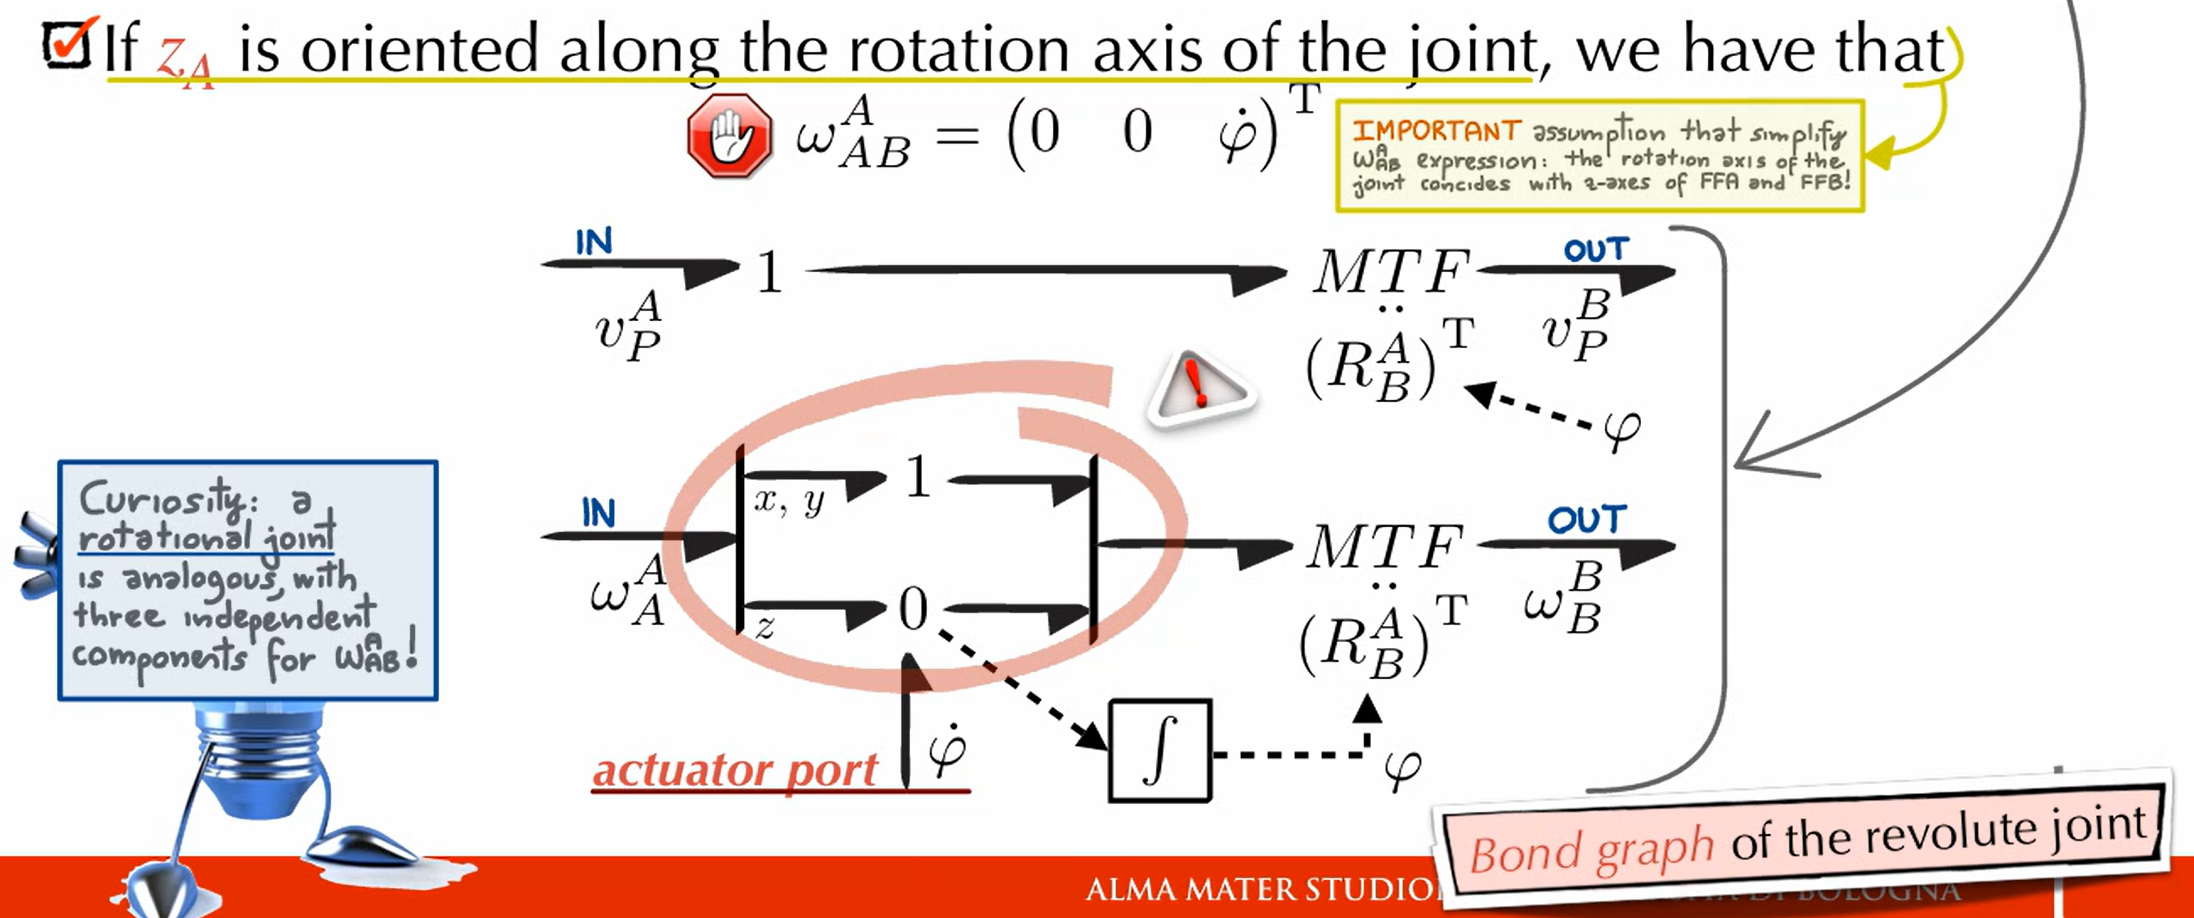
\includegraphics[width=0.8\textwidth]{figs/chapter6/6_9.png}
  \caption{Bond graph of a revolute joint between two rigid bodies, showing the velocity constraints and the free rotational degree of freedom.}
\end{figure}



\paragraph{Translational (Prismatic) joint.}
A prismatic joint fully constrains angular velocities among the bodies ($\boldsymbol{\omega}_A = \boldsymbol{\omega}_B$), meaning they always have the same relative orientation. The relative linear velocity is constrained to one direction $\hat{\mathbf{d}}(\theta)$ (which itself varies as the mechanism rotates). A force $F_r$ acts along this direction. Assuming the translation axis coincides with the $z$-axis of both frames, $\mathbf{v}_{AB}^A = (0, 0, \dot{s})^T$. The constraint and the direction transformation involve MTF elements with time-varying moduli that depend on the current configuration angle $\theta$.

\begin{figure} [H]
  \centering
  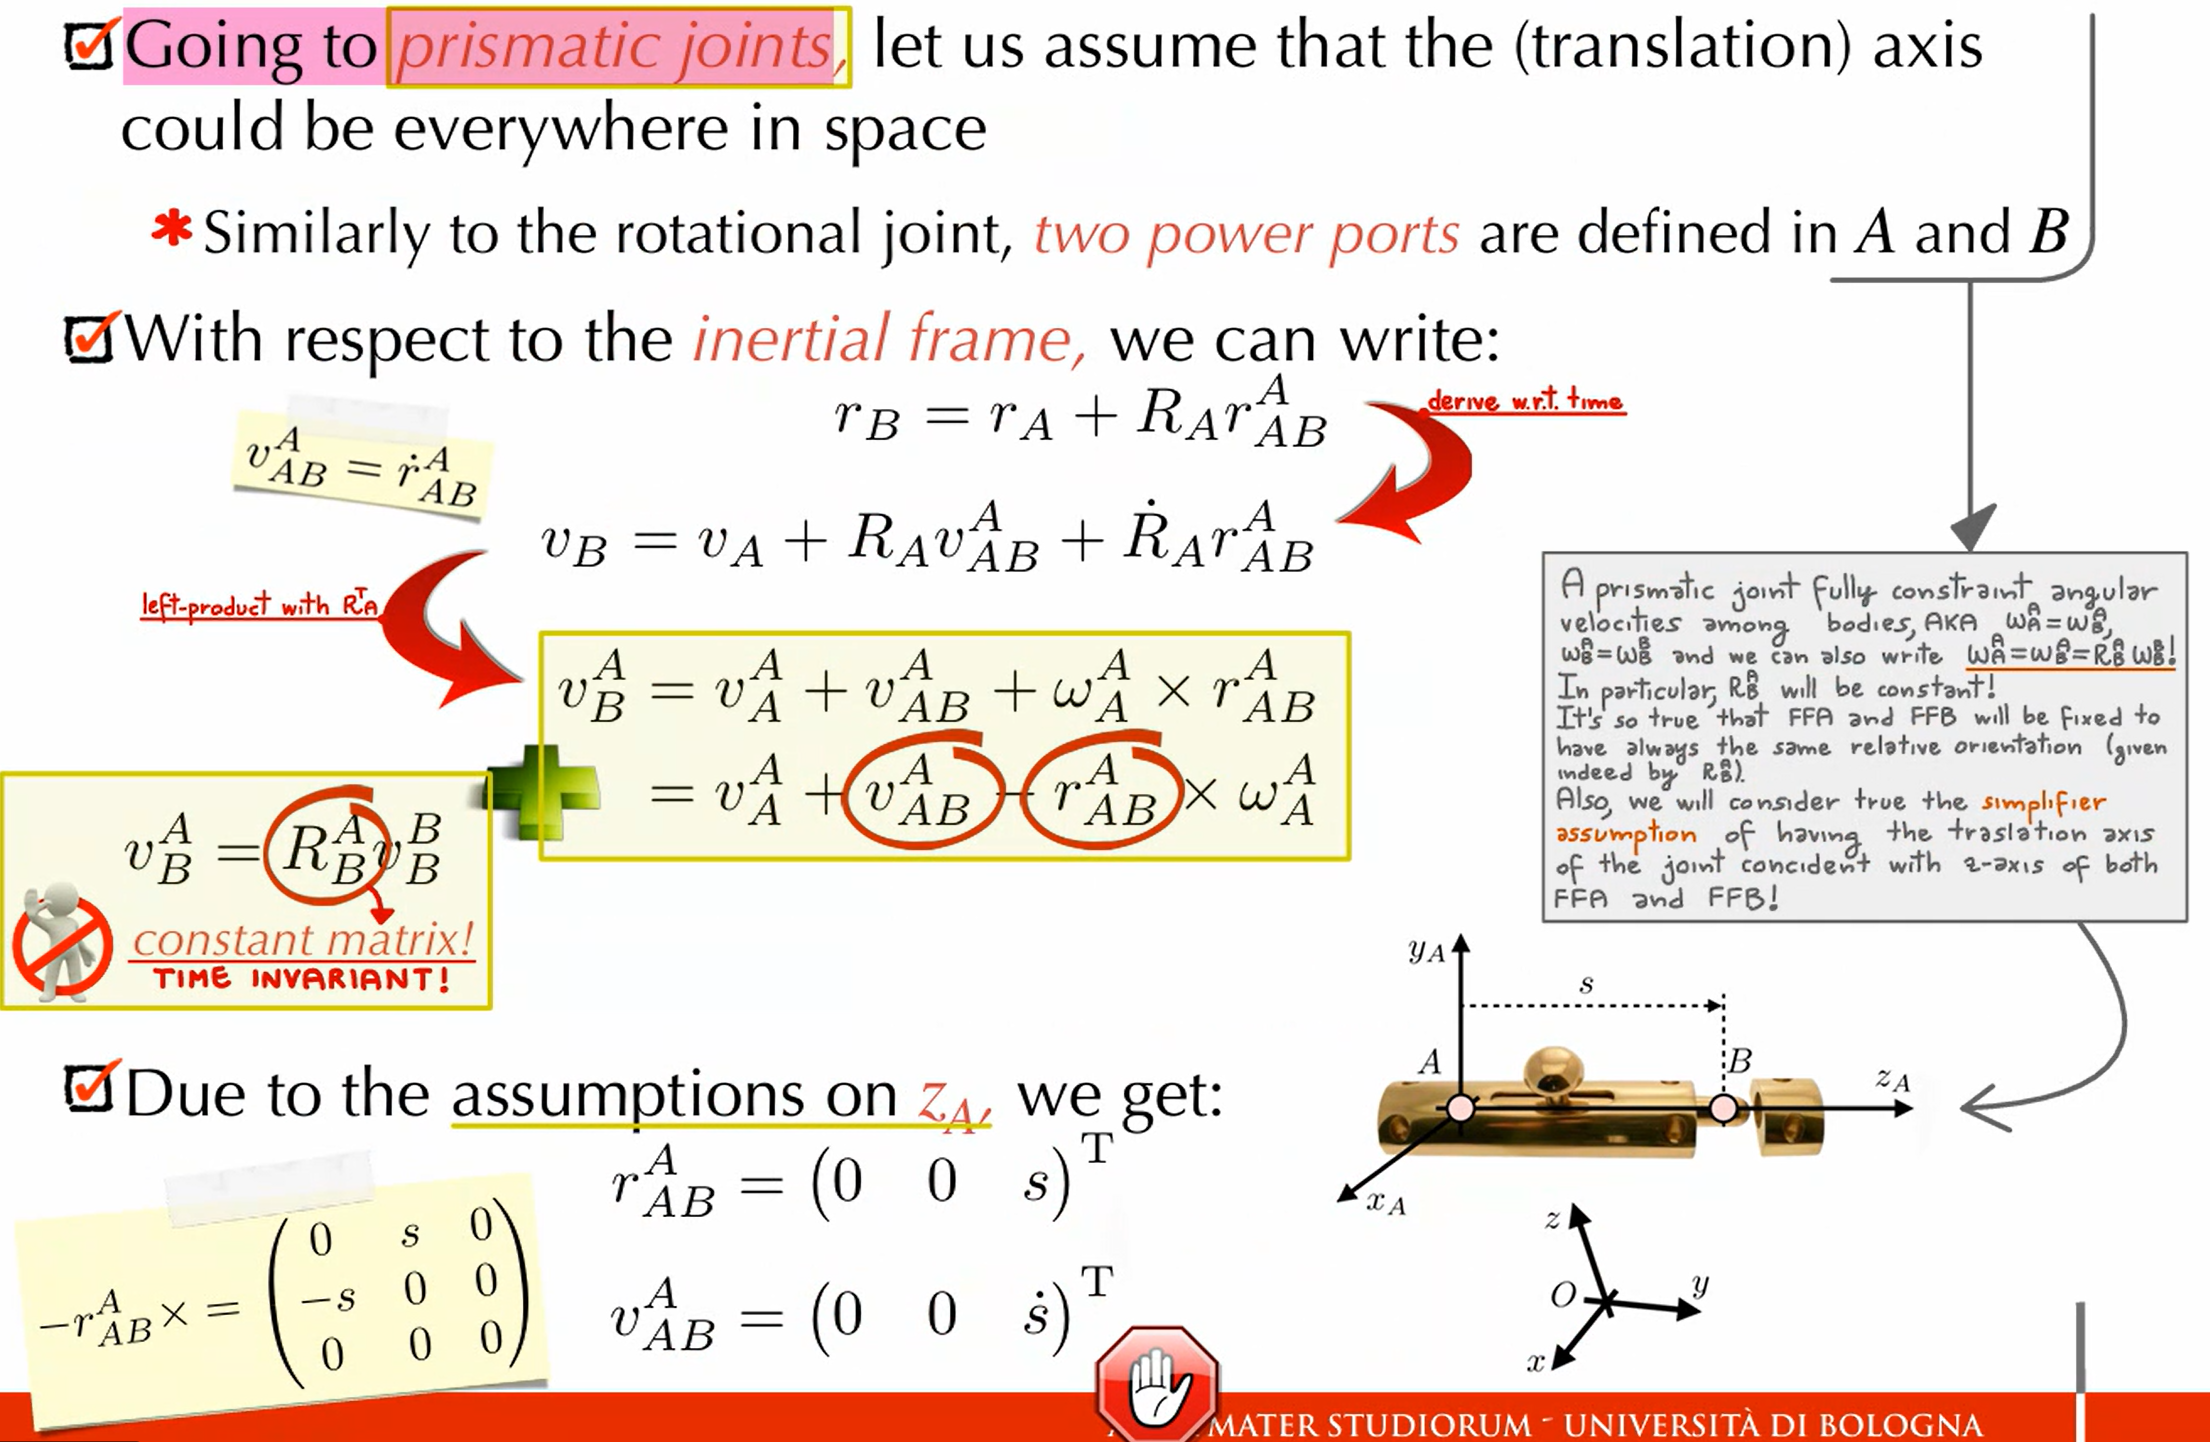
\includegraphics[width=0.8\textwidth]{figs/chapter6/6_10.png}
  \caption{Derivation of equations for a prismatic joint, plus assumption of Denavit--Hartenberg convention for the joint axis.}
\end{figure}


The key practical point is: in the inertial-frame formulation, joint directions $\hat{\mathbf{d}}(\theta)$ are time-varying, making the MTF moduli time-varying. This is why the \textbf{body-frame formulation} is typically preferred for multi-body dynamics — joint directions remain constant in the body frame.

\begin{figure} [H]
  \centering
  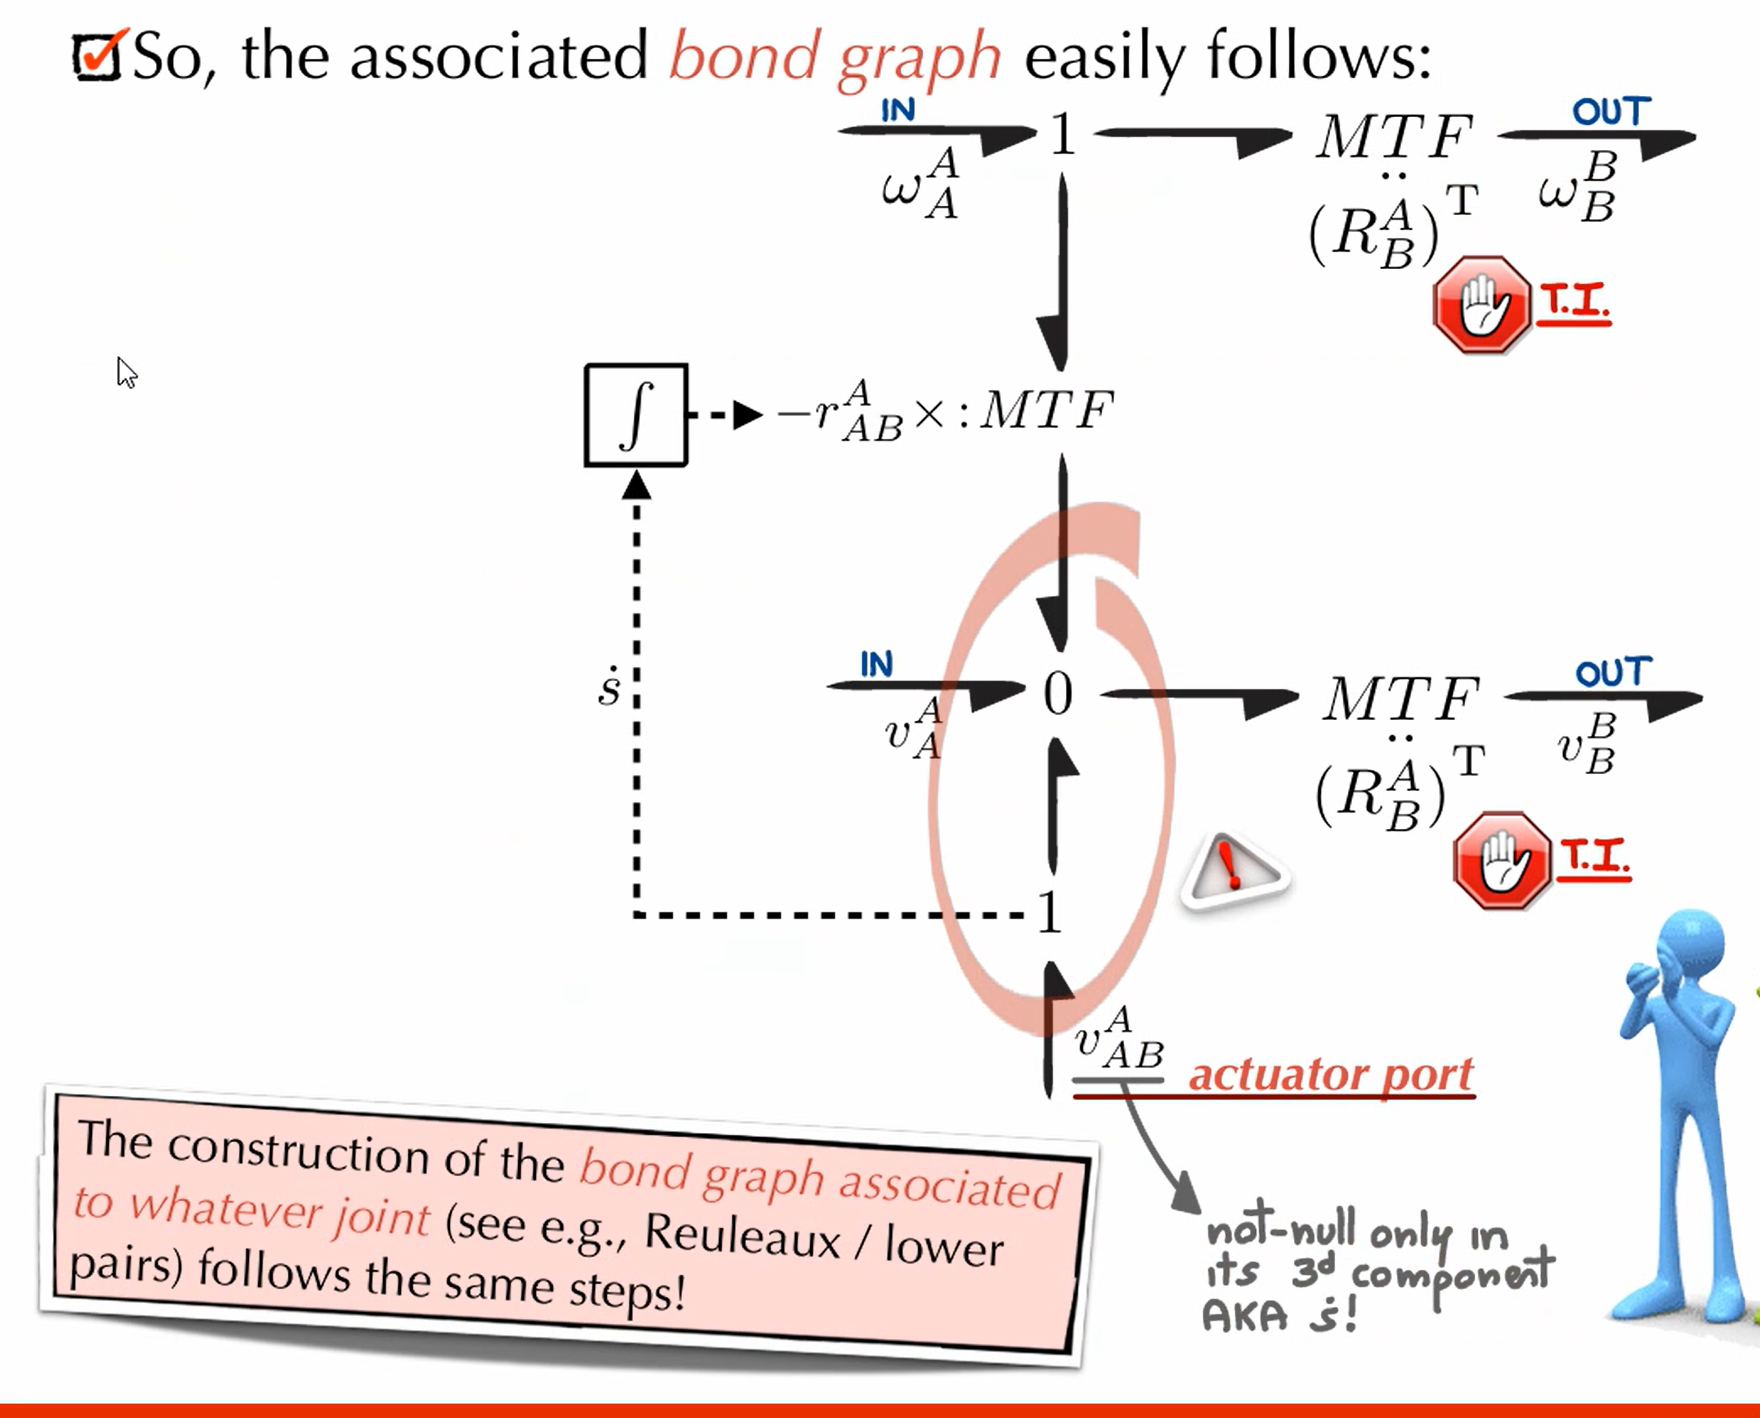
\includegraphics[width=0.8\textwidth]{figs/chapter6/6_11.png}
  \caption{Bond graph of a prismatic joint between two rigid bodies, showing the angular velocity constraints and the linear velocity constraint along the prismatic axis.}
\end{figure}







\section{Kinematic nonlinearities in the dynamics}

Main drawback is that the final equations are nonlinear and with (integrable) constraint. Up to now we just used the kinematic constraints to write the bond graph, we haven't yet introduced the dynamics of the system. For simpler systems using the proposed method is too complex.

We must find a convenient way to describe the system without the rigid body dynamics. We'll use a \textbf{standard model}. 


For any problem in mechanics involving particles, rigid bodies and elastic elements, the mathematical model consists of a set of first order ODEs in terms of variables with some physical insight.

Equations are \textbf{coupled} and \textbf{explicit}. 

\begin{align}
  f_C = \Phi_C^{-1} (q_C) \\
  v_I = \Phi_I^{-1} (p_I) \\
  \dot{q}_C = T_{CI} (q_C) v_I \\
  \dot{p}_I = - T_{CI}^T (q_C) f_C
\end{align}


The most difficult aspect is the nonlinear coupling of C- and I- fields introduced by the geometry of large-scale motions, i.e. $T_{CI}(q_C)$ by that is associated with multiport displacement-modulated transformers

Forces and velocities $(f_C, v_I)$ can be eliminated which gives:

\begin{equation*}
  \dot{q}_C = T_{CI}(q_C) \Phi_I^{-1} (p_I), \qquad
  \dot{p}_I = - T_{CI}^T (q_C) \Phi_C (q_C)
\end{equation*}

\begin{figure} [H]
  \centering
  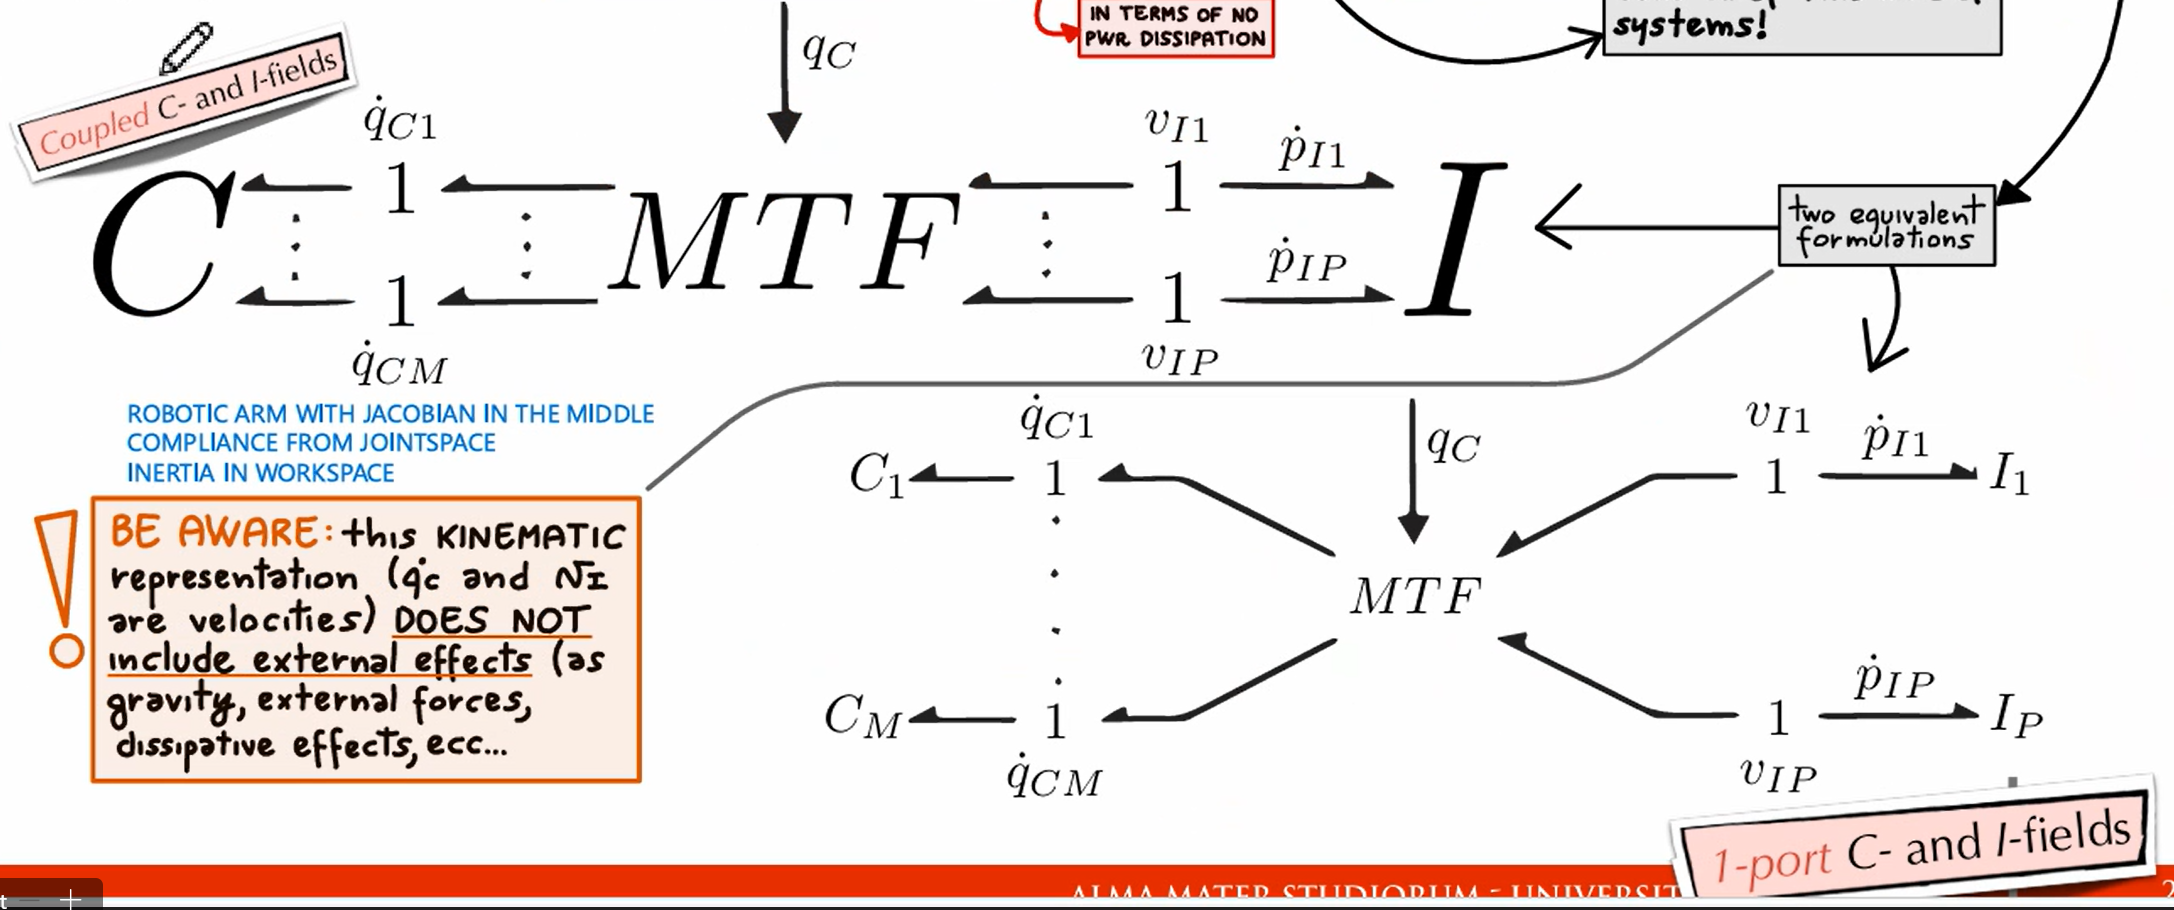
\includegraphics[width=0.8\textwidth]{figs/chapter6/6_12.png}
  \caption{Basic nonlinear conservative system}
\end{figure}

Here is an example with the spring-pendulum. Notice that it's possible to add external forces. 

\begin{figure} [H]
  \centering
  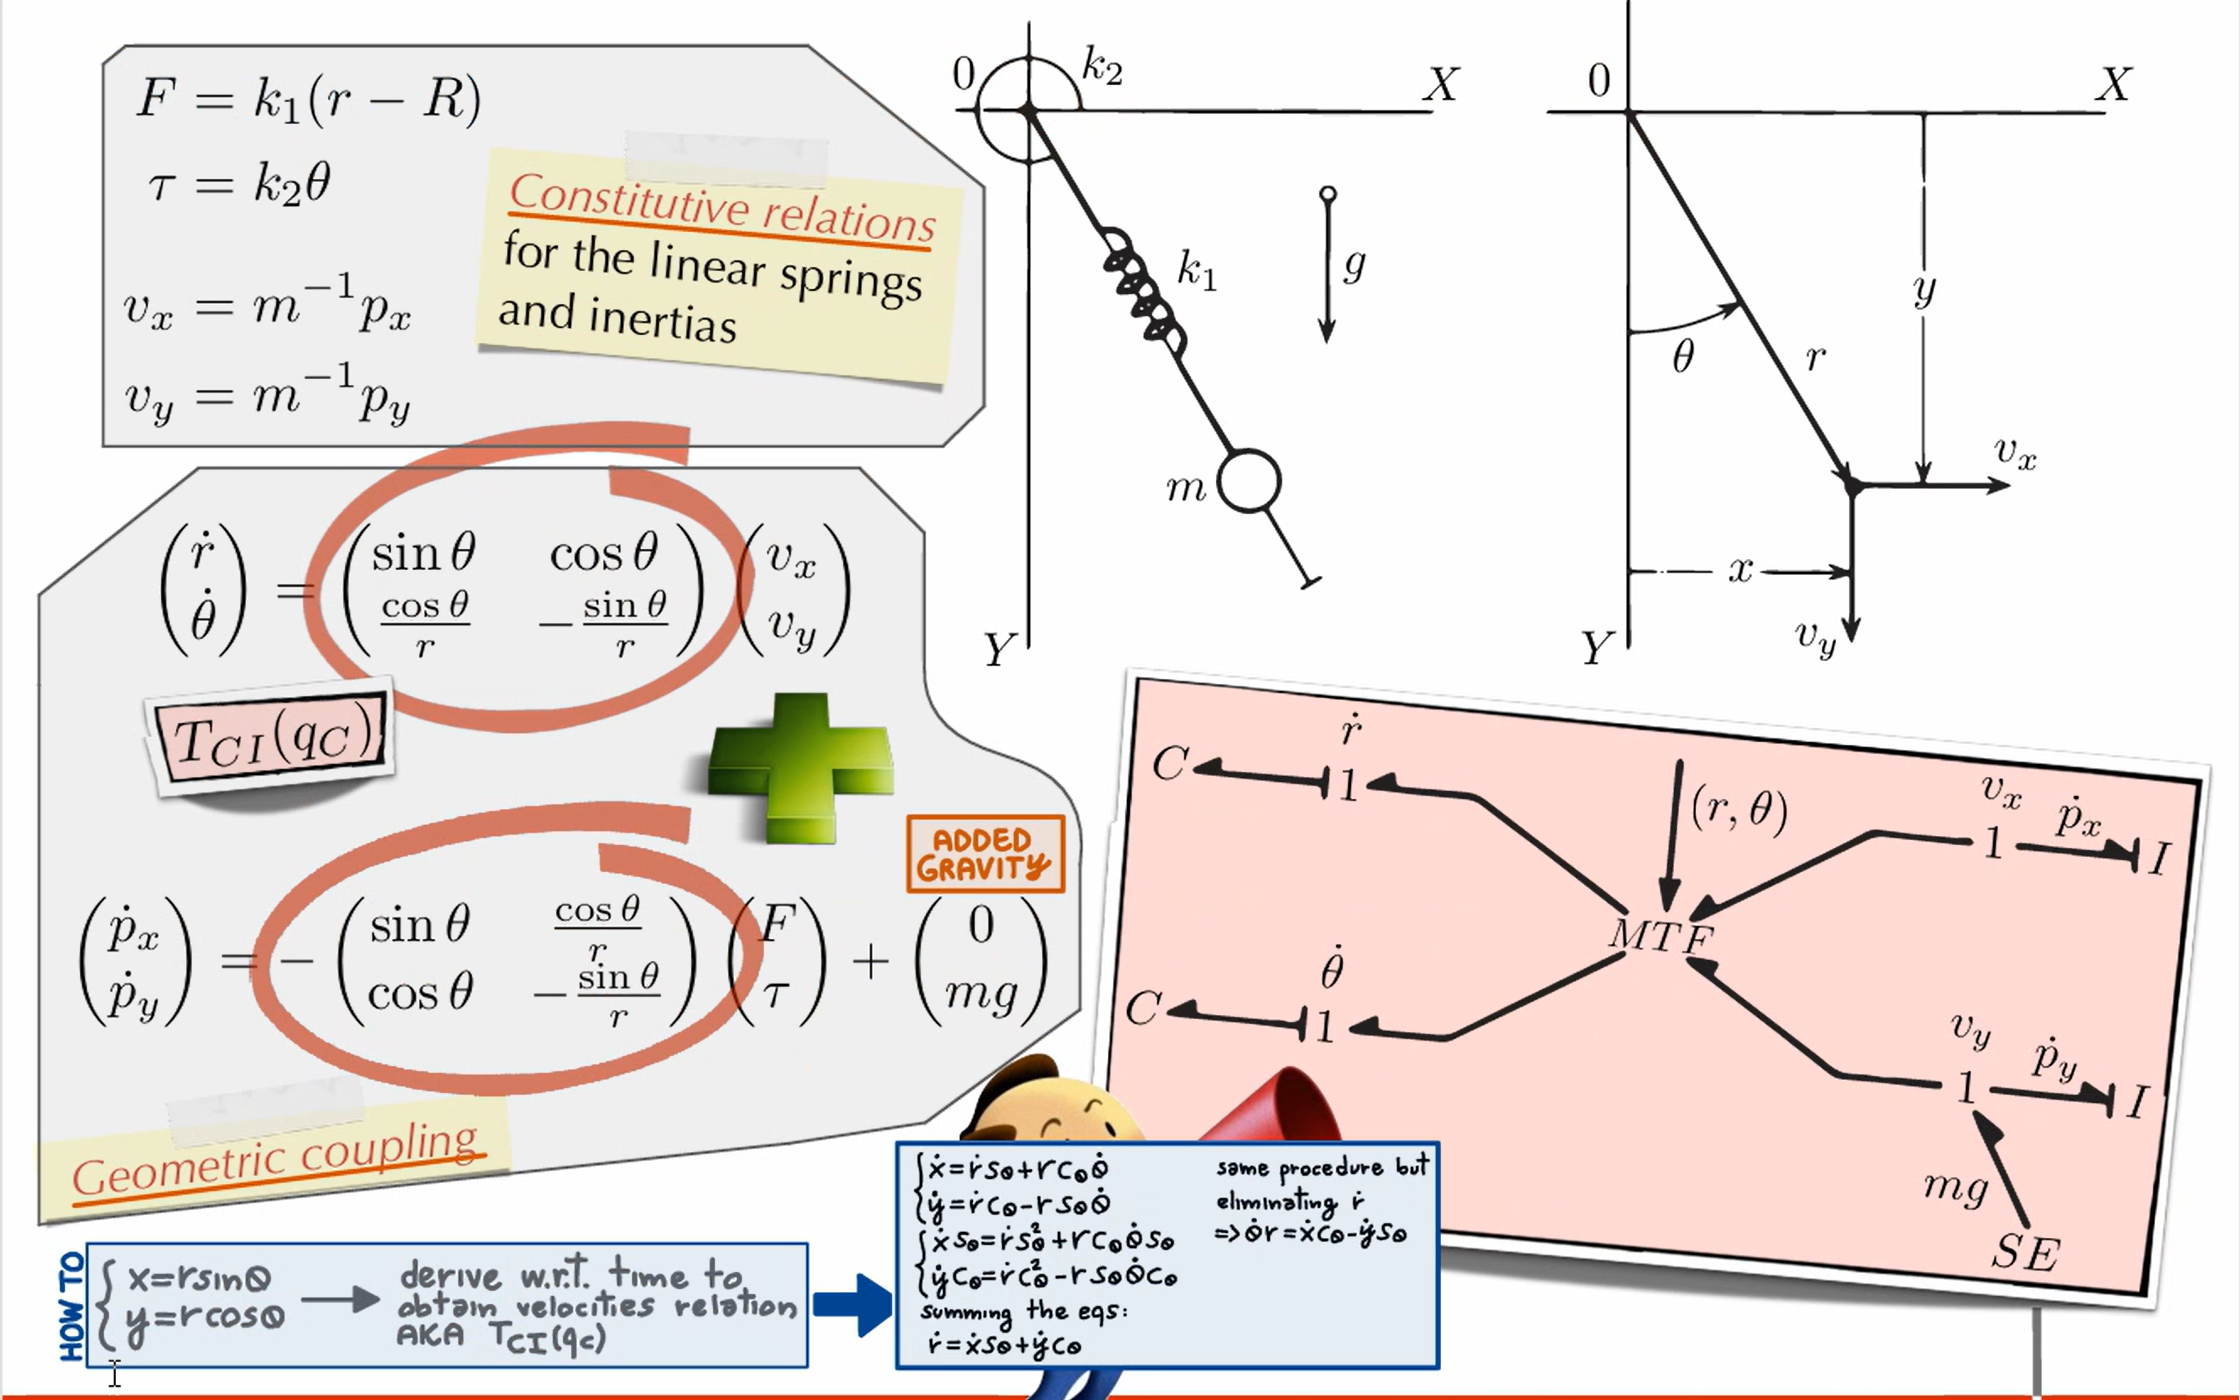
\includegraphics[width=0.8\textwidth]{figs/chapter6/6_13.png}
  \caption{Spring pendulum example}
\end{figure}

This is a conservative system, so there are no damping terms. 


\section{The K.A.M. (Kinematic Analysis Method)}

Before addressing closed loops and derivative causality, it is useful to formalize how to build a mechanism's bond graph starting purely from kinematics.
\begin{enumerate}[leftmargin=2em,itemsep=2pt]
  \item \textbf{Identify key variables}: Determine the vector of generalized coordinates $\mathbf{q}_k$, the C-field displacements $\mathbf{q}_C$, and the I-field velocities $\mathbf{v}_I$. Note that this method works with velocities (flows).
  \begin{enumerate}
    \item If the vector containing the time derivatives of the generalised coordinates  $q_k$ represents a necessary and sufficient set of velocities to fix all the motions at any instant, then the system is holonomic
  \end{enumerate}
  \item \textbf{C-field constraints}: Relate $\mathbf{q}_C$ to $\mathbf{q}_k$ and differentiate to get $\dot{\mathbf{q}}_C = \mathbf{T}_{Ck}(\mathbf{q}_k)\dot{\mathbf{q}}_k$. Write this into the bond graph using MTFs and 0-junctions.
  \item \textbf{I-field constraints}: Obtain the velocity transformation $\mathbf{v}_I = \mathbf{T}_{Ik}(\mathbf{q}_k)\dot{\mathbf{q}}_k$ and append to the graph via MTFs.
  \item \textbf{Attach elements}: Append C- and I-fields to their respective junctions. Add dissipation, gravity (as SE), and simplify the MTFs where possible.
\end{enumerate}



This kinematic description uses a junction structure that links flows (assumed to depend on C-energy variables) to couple C-fields and I-fields. However, this procedure often leads to bond graphs with algebraic loops or derivative causality when bodies are rigidly constrained.


\paragraph{}
The procedure is often successful at deriving a bond graph what will yield state equations easily but it can lead to algebraic loops or with derivative causality. 
A serious problem occurs when two rigid bodies are constrained in a non-flexible way. 


\section{Introduction to DAEs vs ODEs}
In standard Ordinary Differential Equations (ODEs), the system states are defined by explicit derivatives (e.g., accelerations), which a numerical solver integrates to find velocities and positions. A Differential-Algebraic Equation (DAE) introduces algebraic constraints alongside differential equations. The solver must satisfy both the integration steps and the strict algebraic rules simultaneously.

\section{Major Problems with DAEs}
\subsection{The Index Problem (Hidden Derivatives)}
Standard solvers integrate derivatives, meaning they cannot directly handle pure algebraic equations (which lack time derivatives). To solve the system, the algebraic constraint must be differentiated with respect to time until the required derivatives appear. The number of differentiations required is called the \textbf{Differential Index}. Most rigid multibody systems are Index-3 DAEs, which are mathematically heavy and unstable to solve directly.

\subsection{Constraint Drift}
When an algebraic constraint (e.g., position) is differentiated into a velocity or acceleration constraint, the solver ensures only the differentiated constraint is met. Due to tiny numerical truncation errors during integration, the uncorrected position variables will slowly diverge from the original algebraic constraint, causing the physical system to literally drift apart.

\section{Classic Example: The Rigid Pendulum}
Consider a pendulum with mass $m$ attached to a rigid, massless rod of length $L$. Modeled in Cartesian coordinates $(x, y)$, this forms a DAE.

\textbf{1. Differential Equations (Newton's Laws):}
Using $\lambda$ for the unknown tension magnitude:
\begin{align}
m\ddot{x} &= -x\lambda \
m\ddot{y} &= -y\lambda - mg
\end{align}

\textbf{2. Algebraic Equation (The Constraint):}
The rigid rod forces the mass to remain on a circle of radius $L$:
\begin{equation}
x^2 + y^2 - L^2 = 0
\end{equation}

\textbf{Solving and Drift:}
Since $\lambda$ does not appear in the constraint, we must differentiate the constraint twice (Index-3) to find the accelerations:
\begin{equation}
2x\ddot{x} + 2\dot{x}^2 + 2y\ddot{y} + 2\dot{y}^2 = 0
\end{equation}
Substituting Newton's laws into this allows us to solve for $\lambda$. However, because the solver is now strictly enforcing the \textit{acceleration} constraint, microscopic integration errors accumulate over time. The solver forgets the original $x^2 + y^2 = L^2$ rule, leading to constraint drift where the rigid rod slowly stretches and breaks apart in the simulation.


\textbf{Constraints} might be enforced by a joint between the bodies. The degrees of freedom are reduced
by the constraints and this always lead to derivative causality. 


\section{Multi-body problem and constraints}

When two rigid bodies are rigidly connected (e.g.\ a robotic link assembly), the degrees of freedom are reduced by the constraints. A rigid body requires six I-elements, but if rigidly connected, their velocities cannot all be independent. The naive bond graph has \emph{velocity constraints} that force some storage elements into derivative causality, signalling an inconsistency in the model. This is the classic \textbf{Multi-Body Problem}.

\subsection{The "Gaps Method" and Lagrange Multipliers (DAE formulation)}
If we treat the constraints mathematically, we define "gap variables" $\boldsymbol{\delta}$ (e.g., horizontal and vertical distances between two theoretically pinned joints) which must vanish ($\boldsymbol{\delta} = \mathbf{0}$). The forces required to enforce these gaps are \textbf{Lagrange Multipliers} ($\boldsymbol{\lambda}$). 
The system is written in a \emph{descriptor form} (a Differential-Algebraic Equation, DAE system), where $E\dot{\mathbf{x}} = A\mathbf{x} + B\mathbf{u}$ and matrix $E$ is singular. The Jacobian of the constraints $\boldsymbol{\Delta} = \partial \boldsymbol{\delta} / \partial \mathbf{q}_k$ relates the velocities ($\dot{\boldsymbol{\delta}} = \boldsymbol{\Delta}\dot{\mathbf{q}}_k$) and the constraint forces ($\mathbf{F}_e = \boldsymbol{\Delta}^T\boldsymbol{\lambda}$). In the bond graph, these appear as external forces opposing the natural motion to keep $\dot{\boldsymbol{\delta}} = 0$.

\subsection{Handling Derivative Causality Physically and Algebraically}
To resolve the derivative causality natively in the simulation, two distinct tricks are widely used:

\paragraph{Method 1: The "Parasitic Spring" (Breaking the Constraint).}
This is a highly practical engineering approach. Physically, two perfectly rigid bodies connected by a rigid joint represent an over-constrained idealisation. In reality, nothing is perfectly rigid; everything flexes. 
The resolution is to introduce a small \textbf{compliance} at the connection. Rather than a rigid bond forcing equal velocities via a strict 1-junction, the joint is modelled as a stiff spring (C-element with large $k$) and a small damper (R-element) between them.
This:
\begin{enumerate}[leftmargin=2em,itemsep=2pt]
  \item Breaks the strict kinematic constraint, restoring all C- and I-elements to integral causality because the masses can now vibrate at slightly different speeds.
  \item Introduces a fast time scale (stiff ODE) associated with the high-frequency compliance vibration. Stiff ODE solvers are required.
  \item Is physically correct — real connections always have some finite stiffness.
\end{enumerate}

\begin{figure} [H]
  \centering
  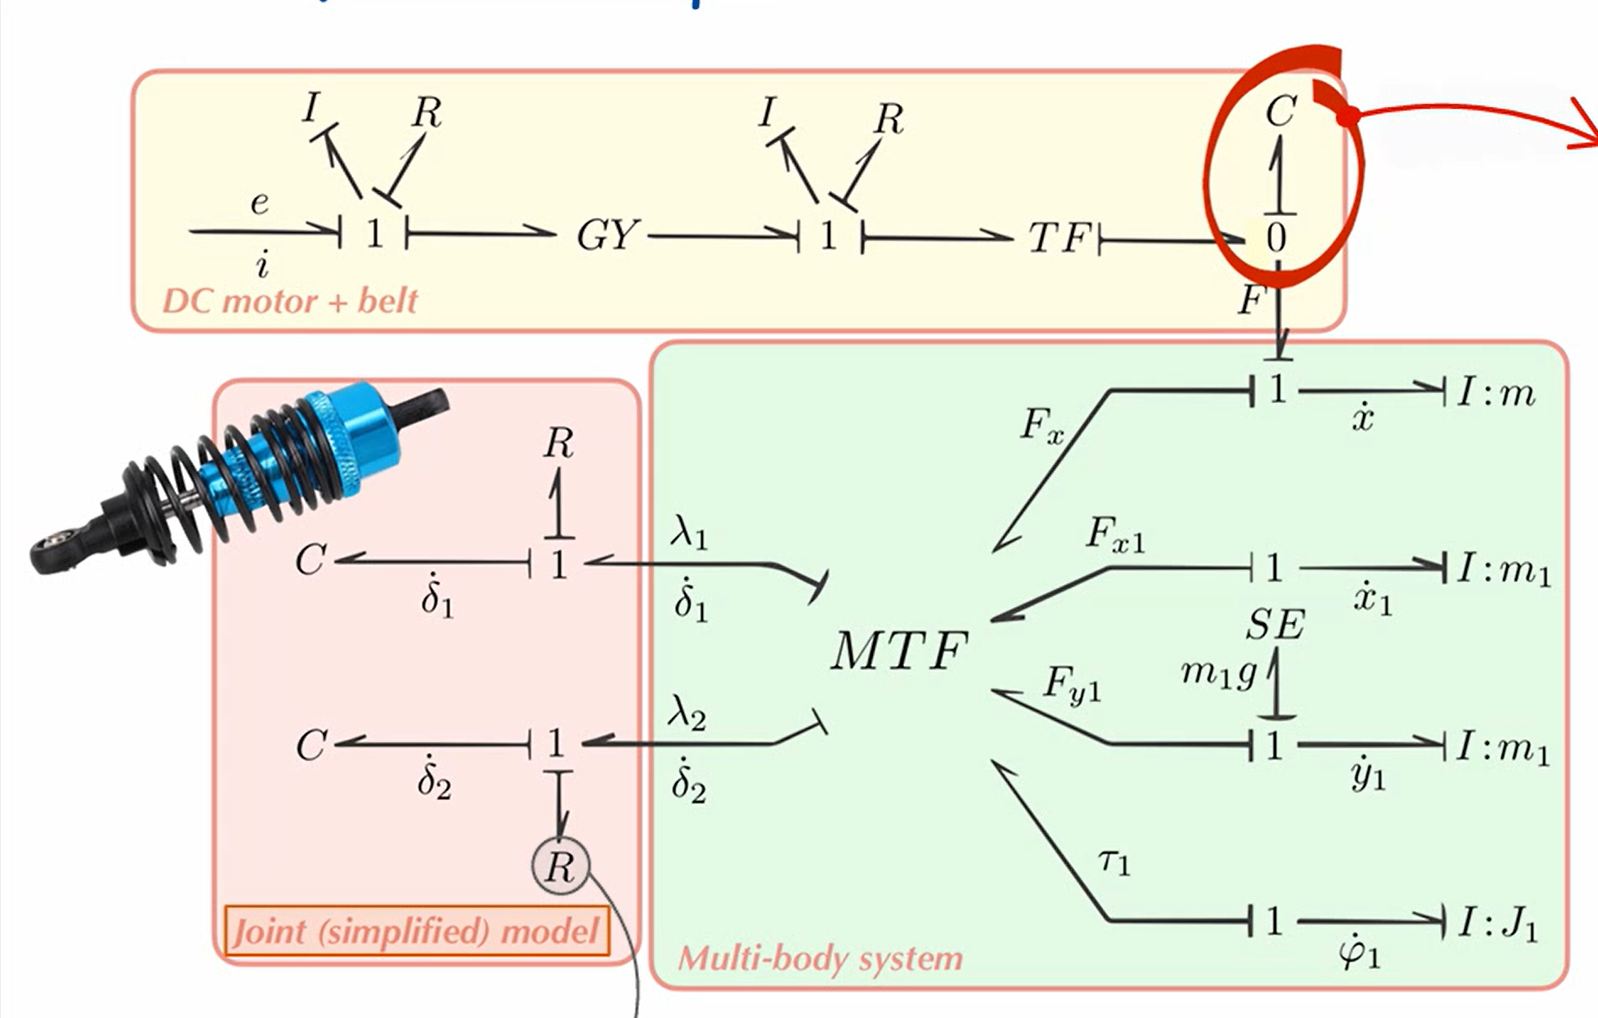
\includegraphics[width=0.8\textwidth]{figs/chapter6/6_14.png}
  \caption{Example of RC simplified model for joint}
\end{figure}



\section{Lagrangian mechanics and IC-fields (D.A.M.)}

The combination of I-fields (kinetic energy) and C-fields (potential energy) in a bond graph with a junction structure encoding kinematic constraints is exactly equivalent to a Lagrangian description. 

If we have a holonomic, lagrange-regular mechanical system, the kinetic energy is a quadratic-affine form: $T = \frac{1}{2}\dot{\mathbf{q}}_k^T \mathbf{M}(\mathbf{q}_k)\dot{\mathbf{q}}_k + \dot{\mathbf{q}}_k^T \mathbf{a}(\mathbf{q}_k)$. 
If $\mathbf{q}_k$ are generalised coordinates, then the Lagrange equations:
\begin{equation}
  \frac{d}{dt}\frac{\partial T}{\partial \dot{q}_i} - \frac{\partial T}{\partial q_i} = E_i
\end{equation}
(where $E_i$ includes potential energy derivatives and external forces) are automatically encoded by the bond graph. The IC-field representation makes this connection explicit and is particularly useful for systems with many degrees of freedom where writing Lagrange equations by hand is error-prone.

It's possible to write the Lagrangian Equations into Hamiltonian equations by the following formulas:

\begin{align}
  p_i = \frac{\partial T}{\dot{q}_i} \\
  \dot{p}_i = \frac{\partial T}{q_i} + E_i \\
\end{align}

where $E_i$ are the generalized forces

The first relation has always a special form:

$$
p_k = M(q_k, t) \dot{q}_k + a(q_k, t)
$$

Therefore we can write: 

$$
\dot{q}_k = M^{-1}(q_k, t) \[p_k - a(q_k, t)
$$

\begin{figure} [H]
  \centering
  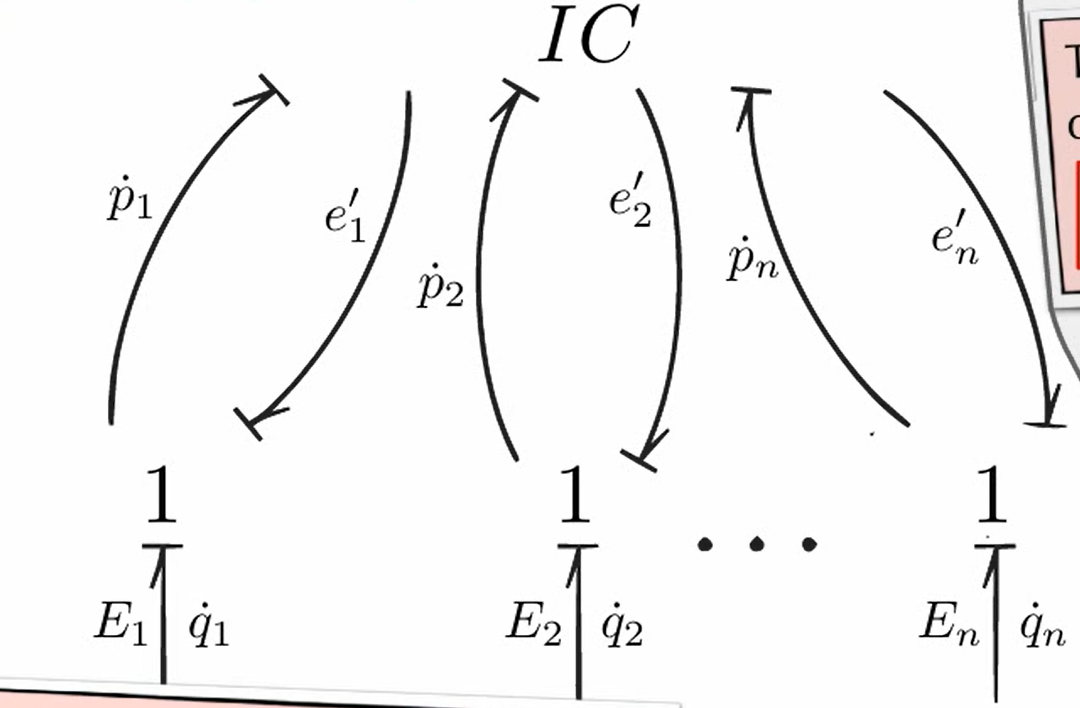
\includegraphics[width=0.8\textwidth]{figs/chapter6/6_15.png}
  \caption{IC field representing the Hamiltonian form of Lagrangian equations}
\end{figure}



\paragraph{The Hamiltonian Form and the D.A.M.}
The \textbf{Dynamic Analysis Method (D.A.M.)} replaces the kinematic junction structure with a true dynamic IC-field based on Hamilton's equations. The Hamiltonian is defined as $\mathcal{H} = \mathbf{p}_k^T\dot{\mathbf{q}}_k - \mathcal{L}$. By defining generalised momenta $\mathbf{p}_k = \partial T / \partial \dot{\mathbf{q}}_k$, we can invert the mass matrix to find velocities:

In the bond graph, the IC-field acts with an I-part computing $\dot{\mathbf{q}}_k$ (flows) from $\mathbf{p}_k$ (momenta), and a C-part computing the internal efforts $\mathbf{e}'_k$ from $\mathbf{q}_k$ (displacements). 

The \emph{main advantage} of this Hamiltonian IC-field approach is that it mathematically guarantees integral causality everywhere, avoiding algebraic loops entirely. The \emph{major drawback} is that the configuration-dependent mass matrix $\mathbf{M}(\mathbf{q}_k, t)$ must be non-singular and continuously inverted during the simulation.
 %══════════════════════════════════════════════════════════════════════
\chapter{Models of Distributed Parameter Systems}
\label{ch:distributed}
%══════════════════════════════════════════════════════════════════════

All models considered so far are \textbf{lumped-parameter models}: the state is a finite-dimensional vector, components are point-like, and the number of degrees of freedom is finite. Real structures, however, have \textbf{continuously distributed} inertia, compliance, and damping — a beam, a gas column, a hydraulic line. These are described by \textbf{partial differential equations} (PDEs), and the number of degrees of freedom is infinite. This chapter develops two strategies for obtaining tractable finite-dimensional bond graph models: \emph{simple lumping} and \emph{separation of variables (normal modes)}.

\section{Distributed vs.\ lumped parameter systems}

A \textbf{distributed-parameter system} is one in which the state (displacement, pressure, temperature, etc.) varies continuously with both time and space. Its model is a PDE of the form:
\begin{equation}
  \mathcal{L}\left[\xi(x,t)\right] = f(x,t),
\end{equation}
where $\mathcal{L}$ is a spatial differential operator and $f$ is a forcing term. The PDE is "local" because it describes the system's behavior point by point. A complete problem statement requires:
\begin{itemize}[leftmargin=2em,itemsep=2pt]
  \item The PDE itself (local dynamics).
  \item \textbf{Initial conditions} at $t = 0$ (as many as the order in time).
  \item \textbf{Boundary conditions} at the spatial extremes $x = 0$ and $x = L$ (as many as the order in space).
\end{itemize}
Only if joined with the proper set of initial and boundary conditions can a PDE be properly solved (yielding a well-posed Cauchy Problem). Notice that a system is typically described with a set of PDEs whose total order is double the space region dimension. 

For linear elastic bodies (isotropic materials), the PDE typically takes the \textbf{wave equation} form:
\begin{equation}
  \frac{\partial^2\xi}{\partial t^2} = c^2\frac{\partial^2\xi}{\partial x^2},
  \quad c = \sqrt{E/\rho},
\end{equation}
with wave speed $c$ determined by the elastic modulus $E$ and density $\rho$. Deformations propagate through the body as waves — a perturbation at $x=0$ does not instantaneously influence $x=L$, but arrives after a delay $L/c$. In a sense, a wave can be mathematically considered as a pair of opposite delays!

\begin{insightbox}[When lumped models fail]
Lumped models assign all inertia to isolated point masses and all compliance to isolated springs with zero mass. This works well when the excitation frequency $\omega$ satisfies $\omega \ll \pi c/L$ (the first natural frequency of the distributed system). When this condition fails — long flexible arms of industrial robots, building floors, transmission lines — distributed effects are essential and lumped models give qualitatively wrong predictions above a certain frequency.
\end{insightbox}

\section{Simple lumping: discretising the continuum}

The most direct approach: \textbf{retain finite-size lumps} instead of taking the limit to infinitesimal elements. For a bar of length $L$, area $A$, density $\rho$, and modulus $E$, divide it into $n$ elements of length $\Delta x = L/n$. Each lump has:
\begin{itemize}[leftmargin=2em,itemsep=0pt]
  \item \textbf{Mass}: $m_i = \rho A\,\Delta x$ (I-element).
  \item \textbf{Compliance}: $C_i = \Delta x/(EA)$ (C-element, from Hooke's law $\sigma = E\,\varepsilon$, $\varepsilon = \partial\xi/\partial x \approx (q_i)/\Delta x$).
\end{itemize}

The generalised momentum and displacement for the $i$-th lump are:
\begin{equation}
  p_i = \rho A\,\Delta x\cdot\dot{\xi}_i \quad\text{(momentum)},
  \qquad q_i = \xi_i - \xi_{i-1} \quad\text{(relative deformation)}.
\end{equation}
The equations for each interior lump read:
\begin{equation}
  \dot{p}_i = \frac{EA}{\Delta x}(q_{i+1} - q_i), \qquad
  \dot{q}_i = \frac{1}{\rho A\,\Delta x}(p_i - p_{i-1}).
\end{equation}
These are the \textbf{discrete Newton and Hooke laws}: Newton's law is a 1-junction constraint (momentum change = net force); Hooke's law is a C-element (displacement = compliance $\times$ force). The first and $n$-th elements must be treated carefully since they are boundary elements, typically requiring the addition of $S_E$ or $S_F$ sources to avoid derivative causality at the boundaries.

\begin{insightbox}[Electrical equivalent of the bar]
There is a direct parallelism with electrical transmission lines. An electrical line can be lumped into elements of length $\Delta x$ having an inductance $L\Delta x$ and capacitance $C\Delta x$. The equations $\dot{p}_i = \frac{1}{C\Delta x}(q_{i+1}-q_i)$ and $\dot{q}_i = \frac{1}{L\Delta x}(p_i-p_{i-1})$ lead to exactly the same wave equation $\frac{\partial^2 p}{\partial t^2} = \frac{L}{C} \frac{\partial^2 p}{\partial x^2}$ when taking the limit $\Delta x \to 0$.
\end{insightbox}

\figplaceholder{Bond graph for n-lump bar: chain of alternating I and C elements with 1-junctions, boundary conditions as sources}{See slides 5--8, pack M07}

\paragraph{Timoshenko beam.}
For a beam, two degrees of freedom per cross-section are needed: transverse displacement $w(x,t)$ and rotation $\phi(x,t)$. $\phi$ is the rotation of the plane cross-section, while $\theta$ is the slope of the neutral axis ($\theta \approx \Delta w / \Delta x$). The shear angle is $\gamma = \theta - \phi$.

The Timoshenko model (which accounts for shear deformation and rotary inertia) introduces per lump:
\begin{itemize}[leftmargin=2em,itemsep=0pt]
  \item Translational mass $\rho A\,\Delta x$ and rotary inertia $\rho I\,\Delta x$ (I-elements).
  \item Bending spring $k_b = EI/\Delta x$ relating moment $M$ to angle difference $\Delta\phi$ (C-element).
  \item Shear spring $k_s = \kappa GA\,\Delta x^{-1}$ relating shear force $V$ to angle--slope difference $\phi - \Delta w/\Delta x$ (C-element). Here $\kappa$ takes into account that shear distribution is not perfectly uniform across the section.
\end{itemize}

Taking the limit $\Delta x \to 0$ recovers the Timoshenko PDEs:
\begin{align}
  \kappa GA\frac{\partial}{\partial x}\!\left(\frac{\partial w}{\partial x} - \phi\right)
    &= \rho A\frac{\partial^2 w}{\partial t^2},\\
  EI\frac{\partial^2\phi}{\partial x^2} + \kappa GA\!\left(\frac{\partial w}{\partial x} - \phi\right)
    &= \rho I\frac{\partial^2\phi}{\partial t^2}.
\end{align}
Neglecting rotary inertia ($\rho I \approx 0$) and assuming $\kappa GA \to \infty$ (infinitely stiff in shear, so $\gamma \to 0$ and $\theta = \phi = \partial w / \partial x$) recovers the simpler \textbf{Euler--Bernoulli model}:
\begin{equation}
  EI\frac{\partial^4 w}{\partial x^4} + \rho A\frac{\partial^2 w}{\partial t^2} = q(x,t),
\end{equation}
where $q(x,t)$ is the distributed transverse load. 
\figplaceholder{Bond graph for Timoshenko beam lump i: two I-elements (translational and rotary) + two C-elements (bending and shear) per cell}{See slides 10--12, pack M07}

\paragraph{Limitations of simple lumping.}
The key drawback is the \textbf{accuracy--complexity trade-off}: each additional lump improves the prediction of low-frequency behaviour but simultaneously introduces new, highly inaccurate high-frequency modes. A model with $n$ lumps has $2n$ modes, but only the lowest $\sim n/3$ are reasonably accurate. Worse, the stiff high-frequency modes impose severe constraints on integration time step. Also, it is difficult to analytically predict the convergence to the continuous model. This motivates the separation of variables approach.

\section{Separation of variables and normal modes}

\begin{warningbox}[Major Limitation]
The Separation of Variables method works beautifully and provides spectrally exact representations, but it works \textbf{ONLY for linear PDEs}. If your system includes nonlinear distributed effects, you are forced to solve the continuum equations numerically or back up into a finite lumping representation.
\end{warningbox}

The idea is to seek solutions of the PDE as products of a spatial function and a temporal function: $\xi(x,t) = Y(x)\,\eta(t)$. Substituting into the unforced wave equation (for the bar):
\begin{equation}
  \rho\,Y(x)\,\ddot{\eta}(t) = EA\,Y''(x)\,\eta(t)
  \quad\Longrightarrow\quad
  \frac{\ddot{\eta}}{\eta} = \frac{E}{\rho}\frac{Y''}{Y} = -\omega^2,
\end{equation}
where $-\omega^2$ is a separation constant (negative for oscillatory solutions). This yields two \textbf{ordinary differential equations}:
\begin{equation}
  \ddot{\eta} + \omega^2\eta = 0, \qquad Y'' + k^2 Y = 0, \quad k^2 = \frac{\rho\omega^2}{E}.
\end{equation}
The spatial ODE has general solution $Y(x) = A\cos kx + B\sin kx$; the constants $A$, $B$, and the eigenvalues $k$ (and hence natural frequencies $\omega_n$) are determined by the \textbf{boundary conditions}. 

\paragraph{Example: bar fixed at $x=0$, free at $x=L$.}
Boundary conditions: $Y(0) = 0$ (fixed, zero displacement) and $Y'(L) = 0$ (free, zero stress). These give $A = 0$ and $\cos k_n L = 0$, so:
\begin{equation}
  k_n L = \left(n - \tfrac{1}{2}\right)\pi, \quad n = 1,2,3,\ldots
  \qquad \omega_n = k_n\sqrt{E/\rho} = \frac{(2n-1)\pi}{2L}\sqrt{\frac{E}{\rho}}.
\end{equation}
The corresponding \textbf{mode shapes} (eigenfunctions) are:
\begin{equation}
  Y_n(x) = \sin\left(\frac{(2n-1)\pi x}{2L}\right).
\end{equation}
These are the natural shapes in which the bar can vibrate. If the bar is displaced into the shape of the $n$-th mode and released, it oscillates purely at frequency $\omega_n$. 

\paragraph{Orthogonality.}
Mode shapes of a self-adjoint differential operator are orthogonal with respect to the mass distribution:
\begin{equation}
  \int_0^L \rho A\,Y_m(x)\,Y_n(x)\,dx = 0 \quad \text{for } m \neq n.
\end{equation}
This is the key property that decouples the equations.

\section{Modal decomposition: the forced case and P.F.R.}

To handle external forcing within this continuum formulation, we use the \textbf{Point-Force Representation (P.F.R.)}. An external active force $F(t)$ acting strictly at a point $\tilde{x}$ is described as a force per unit length using the Dirac delta function: $f(x,t) = F(t)\delta(x-\tilde{x})$. 

The response to this force is written as a superposition of all modes:
\begin{equation}
  \xi(x,t) = \sum_{n=1}^\infty Y_n(x)\,\eta_n(t).
\end{equation}
Substituting this into the forced PDE, multiplying by $Y_m(x)$, and integrating over space $x \in [0,L]$, orthogonality eliminates all cross-terms and yields one decoupled ODE per mode. Because of the Dirac delta integral property ($\int F(t)\delta(x-\tilde{x})Y_m(x)dx = F(t)Y_m(\tilde{x})$), the result is:
\begin{equation}
  \boxed{m_n\,\ddot{\eta}_n + k_n\,\eta_n = F(t)\,Y_n(\tilde{x})},
  \qquad m_n = \int_0^L \rho A\,Y_n^2\,dx = \frac{\rho AL}{2}, \quad k_n = m_n\omega_n^2.
\end{equation}
This is the \textbf{modal equation}: a simple harmonic oscillator with mass $m_n$ (modal mass), stiffness $k_n = m_n\omega_n^2$ (modal stiffness), and forcing $F(t)\,Y_n(\tilde{x})$ (the modal forcing factor evaluates the mode shape exactly at the point where the force is applied). The response is found separately for each mode and then combined. 

\section{Bond graph for the finite-mode model}

Introducing modal momentum $p_n = m_n\dot{\eta}_n$ and displacement $q_n = \eta_n$, the modal equation becomes:
\begin{equation}
  \dot{p}_n = -k_n q_n + F(t)\,Y_n(\tilde{x}), \qquad \dot{q}_n = p_n/m_n.
\end{equation}
This is exactly the state equation of an I-element ($I = m_n$) and a C-element ($C = 1/k_n$) on a 1-junction, with the external force $F(t)$ connected via a TF of modulus $Y_n(\tilde{x})$. The \textbf{finite-mode bond graph} is:

\figplaceholder{Bond graph for $N$-mode bar: N parallel I--C pairs (modal oscillators) each connected via TF:Yn(x) to a common port (0-junction) where F is applied}{See slides 23--25, pack M07}

This is the preferred model because:
\begin{enumerate}[leftmargin=2em,itemsep=2pt]
  \item It captures the exact frequency content up to the retained modes.
  \item It has all storage elements in integral causality (when the input is an effort).
  \item It can be seamlessly connected to other bond graph subsystems.
  \item Retaining $N$ modes gives a model of order $2N$ that is spectrally exact up to $\omega_N$.
\end{enumerate}

\begin{insightbox}[Force-free boundary conditions are preferred]
When the boundary conditions are uncertain or may change (e.g.\ a beam whose end attachment varies during operation), it is best to use \textbf{force-free mode shapes} — eigenfunctions of the PDE with zero force (and moment) at all boundaries. These modes can represent any motion, including motions at previously ``fixed'' boundaries (by attaching a stiff spring to ground later), whereas modes derived for a fixed boundary can never generate motion there. Force-free modes are harder to derive but provide a universal modelling library.
\end{insightbox}

\paragraph{Rigid Body Modes.}
When using force-free boundaries, the frequency equation permits $\omega = 0$. These correspond to \textbf{rigid body modes} where the structure moves without deformation. For a free-free beam, there are two such modes: a pure translation ($Y_{00}(x) = 1$) and a pure rotation about the centre of mass ($Y_0(x) = x - L/2$). In the bond graph, these appear as pure I-elements (modal mass and rotary inertia) without accompanying C-elements, because they have zero modal stiffness ($k=0$).

\paragraph{Reading outputs and applying moments at arbitrary locations.}
The velocity at any point $x_0$ along the bar is:
\begin{equation}
  \frac{\partial\xi}{\partial t}(x_0, t) = \sum_n Y_n(x_0)\,\dot{\eta}_n(t) = \sum_n Y_n(x_0)\,\frac{p_n}{m_n}.
\end{equation}
In the bond graph, this is a 0-junction connected to TF elements of moduli $Y_n(x_0)$, with each mode's velocity read from its I-element. Similarly, forces can be applied at arbitrary interior points by adding zero-force Se sources at those locations — these serve as output measurement points without injecting any power. 

If an external \emph{moment} is applied instead of a force, the associated TF elements coming from the moment 0-junction have the \emph{mode shape slopes} $dY_n(x)/dx$ evaluated at the location of the moment as their moduli, instead of the mode shapes $Y_n(x)$ themselves.

\section{Damping, Mode Selection, and Causality}

\paragraph{Including Damping.}
The separation of variables formulation mathematically works only without damping. However, physical structures are lightly damped (modal damping ratio $\zeta_i \in [0.01, 0.1]$). Instead of modeling the complex physical damping distribution, we functionally insert damping into the individual modes. The modal equation becomes:
\begin{equation}
  m_i\ddot{\eta}_i + b_i\dot{\eta}_i + k_i\eta_i = F_{modal}
\end{equation}
In the bond graph, this is simply an R-element attached to the $i$-th modal 1-junction, with damping constant $b_i = 2\zeta_i\omega_i m_i$.

\paragraph{How many modes to retain? The Residual Compliance.}
The number of modes retained depends on the expected frequency content of the inputs. Modes whose natural frequency $\omega_i$ is significantly higher than the highest input frequency $\omega_{max}$ operate in the \textbf{stiffness-controlled region}. In this region, the modal inertia and resistance have virtually no effect. 
As a rule of thumb, modes are retained up to a frequency 2 to 5 times higher than $\omega_{max}$. 
For all higher modes, instead of completely pruning them, we can drastically improve the model's static accuracy by consolidating their modal stiffnesses into a single \textbf{Residual Compliance}. In the bond graph, all higher-order modal 1-junctions are removed, and a single $C_{residual}$ is placed at the input 0-junction, where $1/k_r = \sum_{i>N} (Y_i^2)/k_i$.

\paragraph{Causality Issues: Flow Inputs.}
A major problem arises if the external system imposes a velocity (causal flow input) instead of a force. A flow input forces all the TF elements, which in turn forces exactly one I-element of the modes into \textbf{derivative causality}. This completely breaks the decoupling of the modal equations and creates a severe algebraic problem involving the derivatives of the inputs.
\begin{itemize}
    \item \textbf{The Fix:} Derivative causality can be structurally avoided by appending an additional modal compliance (without its associated modal inertia) at the flow input. This additional "parasitic" mode absorbs the flow boundary condition and restores integral causality everywhere. While this introduces an algebraic loop among the modes, it is a constant algebraic loop that can be easily solved once and for all inside the model matrix, unlike the massive difficulties of dealing natively with DAE derivative causality.
\end{itemize}

\paragraph{Assembling complex structures.}
If a complex structure is composed of many elements (e.g., an A-frame built of three uniform beams), a complete model is constructed by building finite-mode bond graphs for each beam and connecting them at their geometric interfaces using junction structures and TFs. Care must be taken at the connection points, as rigid connections force shared velocities which can again introduce derivative causality, solvable via the compliance techniques described above.
 %══════════════════════════════════════════════════════════════════════
\chapter{Thermo-fluid Systems}
\label{ch:thermofluid}
%══════════════════════════════════════════════════════════════════════

Thermodynamics is the \textbf{universal science of physical processes}: every
model constructed so far --- mechanical, electrical, hydraulic, thermal ---
can be studied through its lens.  When C- and I-fields are constrained to
conserve energy, or R-fields are arranged to dissipate power, thermodynamic
arguments are implicitly at work.  Most dynamic models can be characterised
as \textbf{isothermal models}, and much of engineering thermodynamics is
concerned with changes between equilibrium states rather than with the
transient path of change.  When the path itself is relevant --- when we care
about irreversibility and entropy production --- we enter the domain of
\textbf{irreversible thermodynamics}, which involves genuinely non-equilibrium
systems.

The modelling strategy adopted here rests on the assumption that physical
extents and time scales are such that \textbf{local pseudo-equilibrium
conditions} exist: at each instant every identifiable lump of substance can
be treated as if it were in thermodynamic equilibrium, even if the overall
system is not.  Under this assumption it becomes possible to define
meaningful state variables at every instant and to write first-order ODEs for
their evolution.

This chapter develops two complementary threads: the \emph{true bond-graph
representation} of thermodynamic systems (which identifies temperature $T$ as
an effort and entropy rate $\dot{S}$ as a flow, so that $T\dot{S}$ is genuine
power), and a critical re-examination of \emph{fluid-dynamic systems},
including the lumped modelling of fluid inertia and compliance, Bernoulli's
equation, and the challenges introduced by compressibility and mass exchange
through a control volume.

%──────────────────────────────────────────────────────────────────────
\section{Basic thermodynamics in true bond-graph form}
\label{sec:true_bg_thermo}
%──────────────────────────────────────────────────────────────────────

\subsection{Assumptions and notation}
\label{ssec:thermo_assumptions}

We begin with a set of simplifying assumptions that frame the entire
discussion:
\begin{itemize}[leftmargin=2em,itemsep=4pt]
  \item \textbf{Closed system (Lagrangian viewpoint).}  No mass passes
    through the boundary.  The total mass $m$ of the substance is fixed.
  \item \textbf{Pseudo-equilibrium.}  All parts of the substance are at
    essentially identical conditions of pressure, temperature, and density,
    so that a single set of state variables describes the whole lump.
  \item \textbf{No motion, no electromagnetic or surface-tension forces.}
    Under these conditions a \emph{pure substance} has only
    \textbf{two independent properties}; all others are given by the
    \emph{equations of state}.
\end{itemize}

Extensive quantities (volume, internal energy, entropy) for a \emph{unit
mass} are written in lowercase: $v$ (specific volume), $u$ (specific
internal energy), $s$ (specific entropy).  When a mass $m$ of the substance
is involved the corresponding total quantities are:
\begin{equation}
  V = mv, \qquad U = mu, \qquad S = ms.
  \label{eq:extensive}
\end{equation}


\subsection{The Gibbs equation and the internal energy function}
\label{ssec:gibbs}

It is assumed that the \textbf{internal energy per unit mass} $u$ is a
function of the \emph{specific volume} $v$ and the \emph{specific entropy}
$s$:
\begin{equation}
  u = u(v, s).
  \label{eq:int_energy}
\end{equation}
The \textbf{Gibbs equation} relates infinitesimal changes in $u$ to
changes in $v$ and $s$:
\begin{equation}
  \mathrm{d}u = T\,\mathrm{d}s - p\,\mathrm{d}v,
  \label{eq:gibbs}
\end{equation}
where $T$ is the \emph{thermodynamic temperature} (conjugate to entropy)
and $p$ is the \emph{pressure} (conjugate to volume, with a sign because
expansion does work on the surroundings).  In rate form:
\begin{equation}
  \frac{\mathrm{d}u}{\mathrm{d}t}
  = T\,\frac{\mathrm{d}s}{\mathrm{d}t} - p\,\frac{\mathrm{d}v}{\mathrm{d}t}.
  \label{eq:gibbs_rate}
\end{equation}
The first term ($T\dot{s}$) is associated with a flow of heat or,
sometimes, with dissipative work; the second term ($p\dot{v}$) is
associated with \emph{reversible} mechanical power.

Comparing \eqref{eq:gibbs} with the total differential
$\mathrm{d}u = (\partial u/\partial s)\,\mathrm{d}s
+ (\partial u/\partial v)\,\mathrm{d}v$
immediately identifies:
\begin{equation}
  T = \frac{\partial u}{\partial s}, \qquad
  -p = \frac{\partial u}{\partial v}.
  \label{eq:gibbs_partials}
\end{equation}
A useful consistency check is the \textbf{Maxwell reciprocal relation},
which follows from the symmetry of mixed second partial derivatives:
\begin{equation}
  \left.\frac{\partial T}{\partial v}\right|_{s}
  = \frac{\partial^{2}u}{\partial v\,\partial s}
  = \left.\frac{\partial(-p)}{\partial s}\right|_{v}.
  \label{eq:maxwell}
\end{equation}


\subsection{The pure substance as a true bond-graph C-field}
\label{ssec:cfield}

The constitutive laws of the pure substance may be represented by a
\textbf{true bond-graph C-field}, where $T$ and $p$ are the \emph{efforts}
and $s$ and $v$ are the \emph{displacements}:


\begin{figure}
  \centering
  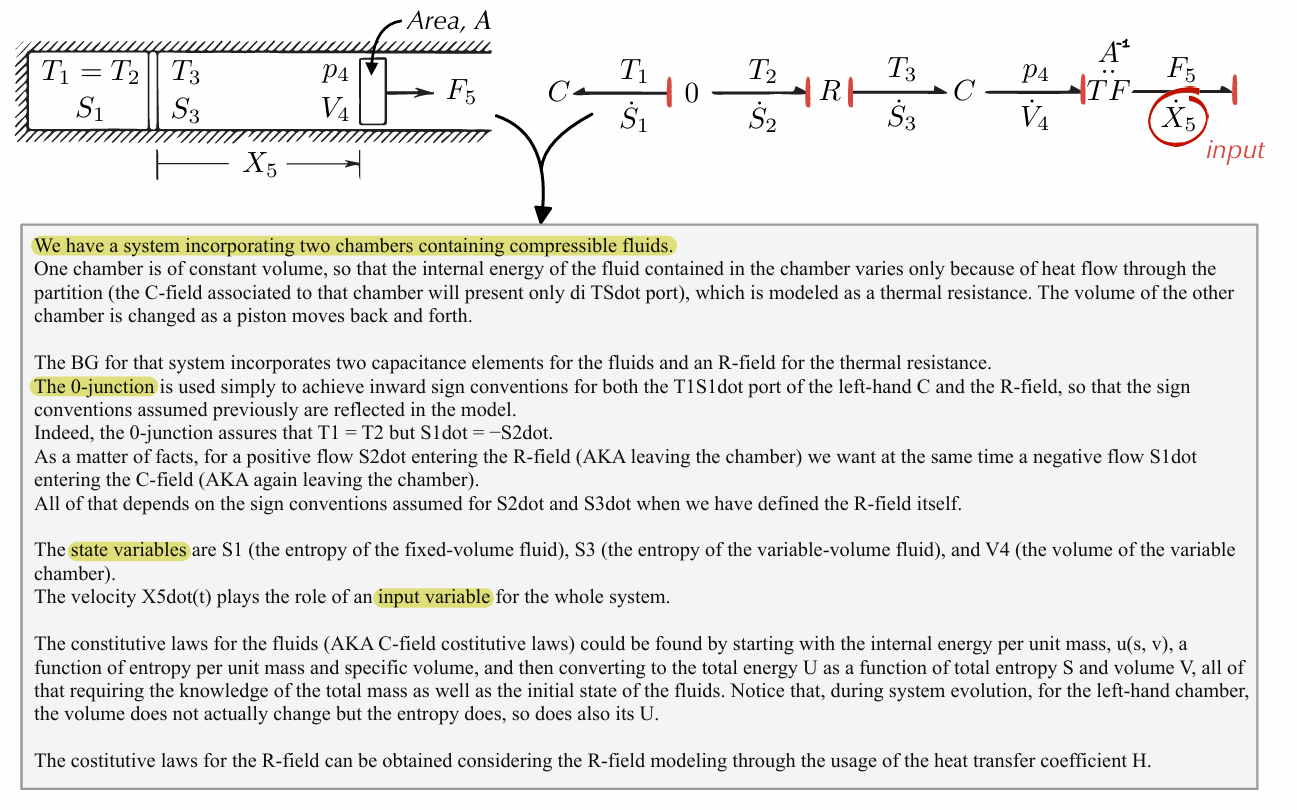
\includegraphics[width=0.6\textwidth]{figs/chapter8/8_1.png}
  \caption{True bond-graph C-field for the pure substance}
\end{figure}



The identification of $T$ as an effort and $s$ as a displacement is the
crucial distinction between a \textbf{true bond graph} and the
\textbf{pseudo-bond graph}: in the true formulation $T\dot{s}$ is genuine
thermodynamic power, whereas in the pseudo-bond graph the product of
conjugate variables is merely a useful analogy (heat flow $\dot{Q}$) and
not a true power.

Under \textbf{integral causality} the C-field is expressed as:
\begin{equation}
  T = T(s, v), \qquad p = p(s, v),
  \label{eq:cfield_integral}
\end{equation}
i.e.\ the efforts are computed from the stored displacements.  For
\emph{mixed-} or \emph{all-derivative causality} the constitutive laws
must be switched around, expressing the displacements as functions of the
efforts.  This inversion is accomplished systematically through the
\textbf{Legendre transformations} of the internal energy $u$.


\subsection{Legendre transformations and causal patterns}
\label{ssec:legendre}

Different causal patterns at the two ports of the C-field correspond to
different Legendre transforms of $u$:

\paragraph{Enthalpy.}  Replace $s$ (displacement) by $p$ (effort) as
independent variable:
\begin{equation}
  h(s, p) = u + pv,
  \qquad
  \frac{\partial h}{\partial s} = T(s,p),
  \qquad
  \frac{\partial h}{\partial p} = v(s,p).
  \label{eq:enthalpy}
\end{equation}
Here the $T$-port retains integral causality ($T$ computed from $s$) while
the $p$-port has derivative causality ($p$ is now an input, $v$ an output).

\paragraph{Helmholtz free energy.}  Replace $s$ by $T$:
\begin{equation}
  f(T,v) = u - Ts,
  \qquad
  \frac{\partial f}{\partial T} = -s(T,v),
  \qquad
  \frac{\partial f}{\partial v} = -p(T,v).
  \label{eq:helmholtz}
\end{equation}

\paragraph{Gibbs free energy.}  Replace both $s$ by $T$ and $v$ by $p$:
\begin{equation}
  \phi(T,p) = u + pv - Ts,
  \qquad
  \frac{\partial \phi}{\partial T} = -s(T,p),
  \qquad
  \frac{\partial \phi}{\partial p} = v(T,p).
  \label{eq:gibbs_free}
\end{equation}

\begin{insightbox}[Why use state functions?]
  Constitutive laws can in principle be written without reference to any
  state function.  The danger is that \emph{arbitrary} constitutive laws
  would not, in general, allow the existence of an internal energy function:
  a substance with such laws could, in a cycle, produce net energy and thus
  act as a \emph{perpetual motion machine of the first kind}.  Deriving
  constitutive laws by differentiating $u$, $h$, $f$, or $\phi$ is therefore
  always safer, since conservation of energy is \emph{automatically} built
  into the relations.  The C-field derived from a Legendre transform is
  guaranteed to be conservative.
\end{insightbox}


\subsection{The perfect gas: Helmholtz free energy route}
\label{ssec:perfect_gas}

A classical example of a constitutive law \emph{not} stated in terms of
state-function derivatives is the \textbf{perfect gas law} (per unit mass):
\begin{equation}
  pv = RT,
  \label{eq:perfect_gas}
\end{equation}
where $R$ is the specific gas constant and $u$ is a function of temperature
$T$ only (i.e.\ it is independent of $v$).  Equation~\eqref{eq:perfect_gas}
alone is \emph{not} a complete characterisation of the C-field: it also
admits only differential causality on the $T\dot{S}$ port, meaning it
cannot be used in integral causality without supplementary information.

Since the natural causality has $T$ and $v$ as independent variables, it
is appropriate to work with the \textbf{Helmholtz free energy}.  Starting
from $-p(T,v) = \partial f/\partial v = -RT/v$:
\begin{equation}
  f(T,v) = -RT\ln v + \psi(T),
  \label{eq:helmholtz_gas}
\end{equation}
where $\psi(T)$ is an unknown function of temperature alone.  The specific
entropy follows as:
\begin{equation}
  -s(T,v) = \frac{\partial f}{\partial T} = -R\ln v + \frac{\mathrm{d}\psi}{\mathrm{d}T}(T),
  \label{eq:entropy_gas}
\end{equation}
and the internal energy is recovered via $u = f + Ts$:
\begin{equation}
  u(T,v) = f(T,v) + Ts = \psi(T) - T\frac{\mathrm{d}\psi}{\mathrm{d}T}(T).
  \label{eq:u_helmholtz}
\end{equation}
Since $u$ must be independent of $v$ (a consequence of the perfect gas
model), this expression is consistent: the volume dependence cancels.  To
determine $\psi(T)$ completely, additional thermal data are needed.


\subsection{Complete equations of state: constant specific heats}
\label{ssec:specific_heats}

To evaluate the complete equations of state it is necessary to express $u$
in terms of $s$ and $v$.  This requires more information than just
equation~\eqref{eq:perfect_gas} because the gas is a \textbf{2-port C-field}
and two independent constitutive relations are needed.  The standard
assumption is that the \textbf{specific heats are constant}:
\begin{equation}
  c_{p} = \frac{\partial h}{\partial T}
  \quad\text{(specific heat at constant pressure)},
  \qquad
  c_{v} = \frac{\partial u}{\partial T}
  \quad\text{(specific heat at constant volume)}.
  \label{eq:specific_heats}
\end{equation}
Choosing the reference state $(T_{0}, v_{0}, p_{0})$ with $u = s = h = 0$:
\begin{equation}
  u = c_{v}(T - T_{0}), \qquad h = c_{p}(T - T_{0}).
  \label{eq:u_h_linear}
\end{equation}
Taking the partial derivative with respect to $T$ of the enthalpy relation
$h = u + pv = u + RT$ yields $c_{p} = c_{v} + R$, the well-known
\textbf{Mayer relation}.

From the Gibbs equation~\eqref{eq:gibbs} written in terms of $T$ and $v$:
\begin{equation}
  \mathrm{d}s = \frac{\mathrm{d}u}{T} + \frac{p}{T}\,\mathrm{d}v
  = c_{v}\,\frac{\mathrm{d}T}{T} + R\,\frac{\mathrm{d}v}{v},
\end{equation}
which integrates to:
\begin{equation}
  s = c_{v}\ln\frac{T}{T_{0}} + R\ln\frac{v}{v_{0}}.
  \label{eq:entropy_Tv}
\end{equation}
Solving~\eqref{eq:entropy_Tv} for the temperature gives the first complete
equation of state:
\begin{equation}
  \boxed{
    (\ast)\quad
    T = T_{0}\,\mathrm{e}^{s/c_{v}}\!\left(\frac{v}{v_{0}}\right)^{-R/c_{v}}
  }
  \label{eq:T_sv}
\end{equation}
Further manipulations of the Gibbs equation written in terms of $v$ and $p$
yield:
\begin{equation}
  \mathrm{d}s = c_{p}\,\frac{\mathrm{d}v}{v} + c_{v}\,\frac{\mathrm{d}p}{p}
  \quad\Longrightarrow\quad
  s = c_{p}\ln\frac{v}{v_{0}} + c_{v}\ln\frac{p}{p_{0}},
\end{equation}
which inverts to give the second complete equation of state:
\begin{equation}
  \boxed{
    (\ast\ast)\quad
    p = p_{0}\,\mathrm{e}^{s/c_{v}}\!\left(\frac{v}{v_{0}}\right)^{-c_{p}/c_{v}}
  }
  \label{eq:p_sv}
\end{equation}
Equations~\eqref{eq:T_sv} and~\eqref{eq:p_sv} are the \textbf{complete
relations for the C-field}.  Substituting~\eqref{eq:T_sv} back into
$u = c_{v}(T - T_{0})$ yields the internal energy as an explicit function
of the state variables $(s,v)$:
\begin{equation}
  u(s,v) = c_{v}T_{0}\!\left[
    \mathrm{e}^{s/c_{v}}\!\left(\frac{v}{v_{0}}\right)^{-R/c_{v}} - 1
  \right].
  \label{eq:u_sv}
\end{equation}
One can verify directly that $T = \partial u/\partial s$ and
$-p = \partial u/\partial v$, confirming consistency with the Gibbs
equation.

\begin{warningbox}[The perfect gas law is not enough]
  Remember that $pv = RT$ is \emph{not} a complete characterisation of the
  C-field.  It also only allows differential causality on the $T\dot{S}$
  port.  The complete description requires both equations~\eqref{eq:T_sv}
  and~\eqref{eq:p_sv}, and these in turn require knowledge of $c_{v}$ in
  addition to $R$.
\end{warningbox}


%──────────────────────────────────────────────────────────────────────
\section{True bond graphs for heat transfer}
\label{sec:heat_transfer}
%──────────────────────────────────────────────────────────────────────

\subsection{The \texorpdfstring{$T\dot{S}$}{TS-dot} port and irreversibility}
\label{ssec:Sdot_port}

The $T\dot{S}$ port of the pure-substance C-field can be used to model
all types of power flow \emph{associated with entropy increase} --- in other
words, all irreversible effects.  Changes in entropy of a pure substance can
be accomplished by a variety of dissipative mechanisms, for example:
\begin{itemize}[leftmargin=2em,itemsep=2pt]
  \item Stirring with a paddle wheel.
  \item Heating with an electrical resistor immersed in a fluid.
\end{itemize}
In each case, the power dissipated can be identified with $T\dot{S}$ in
order to find the change of state of the substance.

An important special use of $T\dot{S}$ ports is in modelling the effects
of \textbf{heat flow}.  If $\dot{Q}$ denotes the rate of heat transfer in
power units, then:
\begin{equation}
  \dot{Q} \;\leftrightarrow\; T\dot{S}.
  \label{eq:heat_power}
\end{equation}
This equivalence is exact in the reversible (quasi-static) limit and
remains a good model for slow, near-equilibrium processes.


\subsection{Two thermal reservoirs and the thermal resistor}
\label{ssec:thermal_resistor}

Consider two \textbf{reservoirs of thermal energy} at temperatures $T_{1}$
and $T_{2}$ communicating through a thermal resistance only (the sides are
perfectly insulated).  Heat $\dot{Q}$ flows from the hotter to the cooler
reservoir.

\begin{figure}
  \centering
  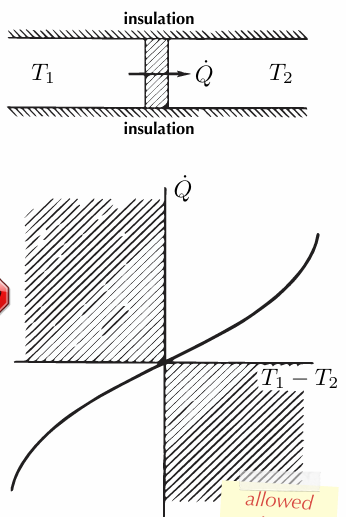
\includegraphics[width=0.5\textwidth]{figs/chapter8/8_2.png}
  \caption{Two perfectly insulated thermal reservoirs at temperatures $T_{1}$ and
  $T_{2}$ ($T_{1} > T_{2}$) connected by a thermal resistor}
\end{figure}

Since the same heat $\dot{Q}$ leaves reservoir 1 and enters reservoir 2,
the power balance at each reservoir gives:
\begin{equation}
  T_{1}\dot{S}_{1} = \dot{Q} = T_{2}\dot{S}_{2}.
  \label{eq:heat_balance}
\end{equation}
The \textbf{net entropy production rate} in the resistor is:
\begin{equation}
  \dot{S}_{2} - \dot{S}_{1}
  = \frac{\dot{Q}}{T_{2}} - \frac{\dot{Q}}{T_{1}}
  = \dot{Q}\,\frac{T_{1} - T_{2}}{T_{1}T_{2}} \geq 0,
  \label{eq:entropy_production}
\end{equation}
which is always non-negative (zero only when $T_{1} = T_{2}$), confirming
the second law.  The entropy flow \emph{leaving} the field is
\emph{greater} than the entropy flow \emph{entering}, regardless of the
direction of heat flow.  This means the thermal resistor is neither a
transformer nor a gyrator: it is an \emph{entropy-generating} element
whose entropy production is independent of the sign of the heat flow.

The thermal resistor is modelled as a \textbf{2-port R-field}:
\begin{equation}
  \frac{T_{1}}{\dot{S}_{1}} \quad R \quad \frac{T_{2}}{\dot{S}_{2}}
  \label{eq:thermal_R}
\end{equation}
This representation differs fundamentally from the pseudo-bond-graph
treatment, where a single scalar resistance connected temperatures and heat
flows.  Here the two entropy-flow ports must be tracked separately because
$\dot{S}_{1} \neq \dot{S}_{2}$.

\begin{insightbox}[The electrical RC analogy has limits]
  It is tempting to model a thermal system exactly like an electrical RC
  network, replacing voltage by temperature and current by heat flow.  This
  analogy is useful but \emph{not} complete: in an electrical resistor the
  current entering equals the current leaving, while in a thermal resistor
  the entropy leaving exceeds the entropy entering.  The analogy between
  electrical and thermal RC systems is therefore not as complete as is often
  assumed.
\end{insightbox}

\paragraph{Constitutive law for the thermal resistor.}
A natural and physically consistent choice is:
\begin{equation}
  \dot{Q} = H(T_{1} - T_{2}),
  \label{eq:thermal_law}
\end{equation}
where $H > 0$ is the \textbf{heat transfer coefficient}.  The individual
entropy flow rates follow from~\eqref{eq:heat_balance}:
\begin{equation}
  \dot{S}_{1} = \frac{H(T_{1} - T_{2})}{T_{1}},
  \qquad
  \dot{S}_{2} = \frac{H(T_{1} - T_{2})}{T_{2}}.
  \label{eq:entropy_rates}
\end{equation}
The \textbf{only admissible causal form} has both temperatures ($T_{1}$ and
$T_{2}$) as inputs and both entropy flows ($\dot{S}_{1}$ and $\dot{S}_{2}$)
as outputs: we cannot impose arbitrary entropy flow rates, because the
constitutive relation~\eqref{eq:entropy_rates} must hold and temperatures
can never be negative.


\subsection{Two compressible chambers: a worked example}
\label{ssec:two_chambers}

As a worked example, consider a system incorporating \textbf{two chambers
containing compressible fluids}:
\begin{itemize}[leftmargin=2em,itemsep=2pt]
  \item One chamber has \emph{constant volume} (the gas is heated or
    cooled only through the thermal resistance).
  \item The other chamber has a \emph{variable volume} whose boundary
    is a piston of area $A$ that can move.
\end{itemize}
The two chambers are separated by the thermal resistance $R$.  The
constitutive laws for the fluids are derived from the total internal energy
$U(S, V)$ of the perfect gas --- specifically, temperature $T$ and pressure
$p$ are found by differentiating $U$ with respect to $S$ and $V$
respectively.

\begin{figure}
  \centering
  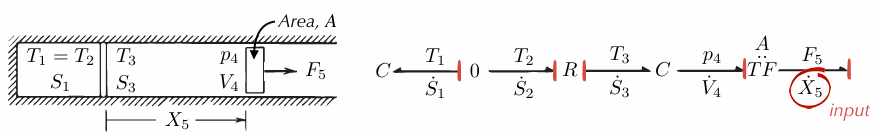
\includegraphics[width=1.0\textwidth]{figs/chapter8/8_3.png}
  \caption{Two-chamber system}
\end{figure}


The model represented by this bond graph is appropriate only for
\textbf{slow changes}: the pseudo-equilibrium assumption requires that
processes occur slowly enough for temperature to be uniform throughout each
chamber at each instant.

Although the entire system is \textbf{power conservative} (no energy is
created or destroyed), the entropy of the two C-elements increases over
time: it appears as if energy is lost.  What the bond graph reveals is that
energy is \emph{not} lost, but rather converted into thermal energy that
\emph{cannot be completely converted back} into mechanical energy --- a
direct manifestation of the second law.  The unique limiting case in which
$X_{5}$ moves so slowly that $T_{2}$ and $T_{3}$ are virtually identical is
the only scenario in which net entropy production almost vanishes.


\subsection{Including Coulomb friction}
\label{ssec:coulomb_friction}

Let us extend the two-chamber model to include \textbf{Coulomb friction}
in the piston.  The friction force is:
\begin{equation}
  F_{6} = A\,\mathrm{sgn}\,\dot{X}_{5},
  \label{eq:coulomb}
\end{equation}
so the dissipated mechanical power is:
\begin{equation}
  F_{6}\dot{X}_{5} = A\dot{X}_{5}\,\mathrm{sgn}\,\dot{X}_{5}
  = A|\dot{X}_{5}| \geq 0.
  \label{eq:friction_power}
\end{equation}
This power is converted entirely into entropy flowing into the adjacent
fluid at temperature $T_{3}$:
\begin{equation}
  \dot{S}_{4} = \frac{1}{T_{3}}\,A|\dot{X}_{5}| \geq 0.
  \label{eq:friction_entropy}
\end{equation}
In bond-graph terms, the mechanical friction is represented as a
\textbf{2-port R-field} connecting a mechanical port and a thermal port.
The R-field can accept either causality at the mechanical port (force or
velocity input), but \emph{only the causality shown} at the thermal port
--- temperature must be an input and entropy flow an output.  The
frictional energy reaches the fluid instantaneously, which is an
idealisation valid when thermal conduction within the fluid is fast
compared to the timescale of interest.


\subsection{Electrothermal resistor}
\label{ssec:electrothermal}

Power dissipation results in thermal effects.  To illustrate the true
bond-graph treatment of mixed energy domains, consider a resistor that
simultaneously carries \textbf{electrical current} and is heated by
\textbf{Joule losses}.  The resistor has a uniform temperature $T$ and
dissipates electrical power:
\begin{equation}
  ei \geq 0,
  \label{eq:joule_positive}
\end{equation}
where $e$ is the voltage and $i$ the current.  If this inequality holds
then both $e$ and $i$ have a ``some'' temperature dependence, because the
resistance is a function of $T$.  The power lost electrically is entirely
converted into heat:
\begin{equation}
  ei = \dot{Q} = T\dot{S}.
  \label{eq:joule_to_heat}
\end{equation}
The R-field has two ports: one electrical ($e$, $i$) and one thermal ($T$,
$\dot{S}$).  There are \textbf{two admissible causal forms}:
\begin{align}
  \text{(a)}\quad e &= e(i, T), &\dot{S} &= \frac{i\,e(i,T)}{T},
  \label{eq:R_causal_a}\\
  \text{(b)}\quad i &= i(e, T), &\dot{S} &= \frac{e\,i(e,T)}{T}.
  \label{eq:R_causal_b}
\end{align}

The temperature of the resistor depends on how much thermal energy has been
stored, so a \textbf{1-port C-element} is necessary to model the thermal
capacity.  It is common to assume $T$ is a linear function of the stored
energy $Q$:
\begin{equation}
  T = T_{0} + \frac{Q}{C},
  \label{eq:T_linear_Q}
\end{equation}
with $\dot{Q} = T\dot{S}$.  However, for the true bond-graph C-element the
constitutive law must express $T$ as a function of the \emph{entropy} $S$:
\begin{equation}
  S = \int_{0}^{S}\mathrm{d}\sigma
  = \int_{0}^{Q}\frac{\mathrm{d}q}{T_{0} + q/C}
  = C\ln\!\left[\frac{1}{T_{0}}\!\left(T_{0} + \frac{Q}{C}\right)\right].
  \label{eq:S_from_Q}
\end{equation}
Inverting gives the true C-field constitutive law:
\begin{equation}
  T = T_{0}\,\mathrm{e}^{S/C},
  \label{eq:T_from_S}
\end{equation}
which is the correct entropy-based form.  Note the nonlinearity: even in
the simple case of constant heat capacity $C$, the true bond-graph
description requires an exponential constitutive law, not a linear one.

\bigskip
\figplaceholder{%
  : the electrical R-field
  (effort $e$, flow $i$) is connected via a 0-junction to the thermal
  C-element (effort $T$, flow $\dot{S}$), with an ambient temperature
  source $T_{0}$ connected via a further R-field representing heat leakage
  to the environment.  Two causal forms of the R-field are shown side by
  side.  Note that the coupling to the ambient can be removed if the
  temperature dependence of the resistance is negligible.}{%
  Slide~17, pack~M08a.}
\bigskip

\begin{figure}
  \centering
  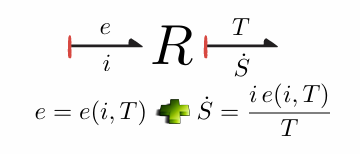
\includegraphics[width=0.6\textwidth]{figs/chapter8/8_4.png}
  \caption{Bond graph for the electrothermal resistor}
\end{figure}


\begin{warningbox}[Only closed systems so far]
  Up to this point, only \textbf{closed systems} have been modelled ---
  no mass crossed the system boundary.  When mass can flow into and out of
  a control volume, the situation becomes significantly more complex and
  requires the introduction of enthalpy convection terms.  This is addressed
  in Section~\ref{ssec:open_volume}.
\end{warningbox}


\subsection{The missing element: no thermal inertia}
\label{ssec:missing_element}

In every energy domain encountered so far (mechanical, electrical,
hydraulic) there is an I-element dual to the C-element.  Let us ask whether
a \textbf{thermal I-element} exists.  In the thermodynamic domain the effort
is temperature $T$ (or temperature difference $\Delta T$) and the flow is
the entropy flow $\dot{S}$.  A hypothetical I-element would obey:
\begin{equation}
  \Delta T = I\,\frac{\mathrm{d}f}{\mathrm{d}t},
  \label{eq:thermal_inertia}
\end{equation}
where $I$ is some parameter (a ``thermal inductance'').
Equation~\eqref{eq:thermal_inertia} implies that $f = \dot{S}$ may have a
\emph{constant non-zero value} even when $\Delta T = 0$: there would be a
sustained entropy (heat) flow in the absence of any temperature difference.

However, the \textbf{second law of thermodynamics} states that a
\emph{spontaneous} heat or entropy flow is \emph{always} directed from a
point of higher temperature to a point of lower temperature.  With an
entropy flow there \emph{must} be a temperature difference.  A thermal
I-element would violate this postulate.  Therefore, \textbf{the I-element
does not exist in the thermodynamic domain}.  This is not a modelling
choice but a fundamental physical constraint.

\begin{insightbox}[``Spontaneous'' means no cross-effects]
  The word ``spontaneous'' in the second-law statement means that no other
  gradients (chemical potential, electric field, etc.) are present that
  might cause cross-effects and drive entropy flow in the absence of a
  temperature difference.  Cross-effects (e.g.\ the Seebeck effect) can
  couple entropy flow to non-thermal driving forces, but these are modelled
  by multi-port elements, not by a thermal I-element.
\end{insightbox}


%──────────────────────────────────────────────────────────────────────
\section{Fluid-dynamic systems revisited}
\label{sec:fluid_revisited}
%──────────────────────────────────────────────────────────────────────

\subsection{Scope and limitations of the bond-graph approach}
\label{ssec:fluid_scope}

The bond-graph models of fluid systems introduced earlier were of the
\textbf{closed-circuit hydraulic type}: static pressure times volume flow
rate ($pQ$) represents most of the transmitted power.  We now take a deeper
look at fluid systems in general and identify the limitations of these
models.

Full \textbf{fluid mechanics} deals with field problems in two or three
dimensions described by PDEs (Navier--Stokes equations), for which
finite-difference or finite-element techniques are required and bond graphs
offer little advantage.  The focus here is therefore:
\begin{itemize}[leftmargin=2em,itemsep=2pt]
  \item The \emph{rough lumping} appropriate when a fluid sub-system is a
    small part of a larger mechatronic system.
  \item \emph{Interior flows} and the fluid-dynamic interaction with solid
    mechanical elements.
\end{itemize}


\subsection{Estimating fluid inertia}
\label{ssec:fluid_inertia}

The I-element represents the inertia of the fluid column.  An elementary
derivation starts from the 1-D assumption: treat the fluid as moving like
a rigid body (quasi-one-dimensional flow) with uniform velocity
$Q/A$ across the cross-section.  Newton's second law for the fluid column of
length $L$ and area $A$ gives:
\begin{equation}
  \rho A L\,\frac{\mathrm{d}}{\mathrm{d}t}\!\left(\frac{Q_{2}}{A}\right)
  = A(p_{1} - p_{3}) = Ap_{2},
  \label{eq:fluid_newton}
\end{equation}
which can be rearranged to:
\begin{equation}
  Q_{2} = \frac{1}{\rho L/A}\,p_{P_{2}},
  \qquad
  I_{\text{fluid}} = \rho L / A
  \quad\text{(inertia coefficient)}.
  \label{eq:fluid_I}
\end{equation}

Several caveats attach to this result:
\begin{itemize}[leftmargin=2em,itemsep=4pt]
  \item The uniform velocity assumption is valid for \emph{transient}
    conditions only approximately; a correcting factor can improve accuracy.
  \item Unless the fluid is \emph{incompressible}, the density $\rho$ is
    not constant and the two ends of the fluid column do not necessarily
    move with the same velocity.
  \item Momentum fluxes at the pipe ends cancel only when the two ends have
    \emph{identical cross-sectional areas}; this derivation does not
    generalise readily to pipes of varying area.
\end{itemize}

\paragraph{The compliance element $C_{6}$.}
The compliance element models the combined compliance of the fluid and pipe
walls.  For small pressure changes the linear capacitor relation is
adequate:
\begin{equation}
  p_{6}(t) = p_{6}(0) + \frac{B}{V_{0}}\int_{0}^{t} Q_{6}\,\mathrm{d}\tau
  = p_{6}(0) + \frac{B}{V_{0}}\,V_{6}(t),
  \label{eq:compliance}
\end{equation}
where $B$ is the bulk modulus and $V_{0}$ the nominal volume.  For
\emph{large} density changes the thermodynamics of the situation must be
studied --- replacing the linear law with a nonlinear one requires a full
thermodynamic analysis (see Section~\ref{ssec:compressible}).

\paragraph{The friction element $R_{4}$.}
The friction element $R_{4}$ represents a pressure loss.  The relation
between $p_{4}$ and $Q_{4}$ is in general \emph{nonlinear}: friction
factor data from experimental fluid mechanics are almost exclusively for
\emph{fully developed steady flow}, making the transient nonlinear
behaviour difficult to capture accurately within a simple lumped model.


\subsection{Bernoulli's equation from the bond-graph viewpoint}
\label{ssec:bernoulli}

To understand the connection between standard fluid mechanics and lumped
bond-graph representation, we derive \textbf{Bernoulli's equation} for
quasi-one-dimensional flow.  This is an extension of the models of M03
and does not involve thermodynamic effects.

We adopt the \textbf{Eulerian method}: let $s$ denote the arc-length
coordinate along the pipe centreline, $v(s,t)$ the average fluid velocity,
$p(s,t)$ the pressure, $A(s)$ the cross-sectional area, and $z(s)$ the
height above a datum.

\begin{figure}
  \centering
  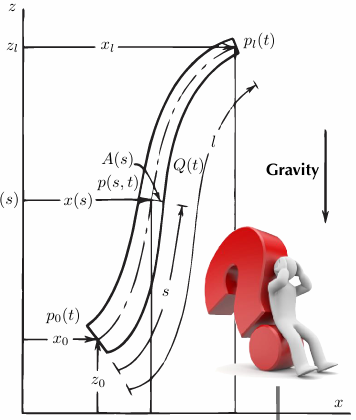
\includegraphics[width=0.4\textwidth]{figs/chapter8/8_5.png}
  \caption{Pipe of varying cross-section}
\end{figure}

\textbf{Newton's law} applied to a fluid element gives the Euler equation
(the \emph{material derivative} $D/Dt$ accounts for both local and
convective acceleration):
\begin{equation}
  \rho\,\frac{Dv}{Dt}
  = \rho\,\frac{\partial v}{\partial t} + \rho v\,\frac{\partial v}{\partial s}
  = -\frac{\partial p}{\partial s} - \rho g\,\frac{\mathrm{d}z}{\mathrm{d}s}.
  \label{eq:euler_eq}
\end{equation}
For an \textbf{incompressible fluid}, continuity requires a constant flow
rate along the pipe:
\begin{equation}
  v(s,t) = \frac{Q(t)}{A(s)}.
  \label{eq:incomp}
\end{equation}
Substituting~\eqref{eq:incomp} into~\eqref{eq:euler_eq} and integrating
along the pipe from $s=0$ to $s=l$:
\begin{equation}
  \rho\left[
    \frac{\dot{Q}(t)}{A(s)}
    + \frac{Q^{2}(t)}{A(s)}\,\frac{\mathrm{d}}{\mathrm{d}s}\!\left(\frac{1}{A(s)}\right)
  \right]
  = -\frac{\partial p}{\partial s} - \rho g\,\frac{\mathrm{d}z}{\mathrm{d}s},
\end{equation}
which integrates to the \textbf{generalised Bernoulli equation}:
\begin{equation}
  \boxed{
    I\dot{Q} + \frac{\rho Q^{2}}{2}\!\left(\frac{1}{A_{l}^{2}} - \frac{1}{A_{0}^{2}}\right)
    = p_{0}(t) - p_{l}(t) - \rho g(z_{l} - z_{0})
  },
  \qquad
  I = \rho\int_{0}^{l}\frac{\mathrm{d}s}{A(s)}.
  \label{eq:bernoulli_bg}
\end{equation}
The first term is the inertia ($I$, with the fluid inertia coefficient
matching~\eqref{eq:fluid_I} for constant $A$); the second term involves
$Q^{2}$ and requires further discussion.


\subsection{Dynamic pressure and the Bernoulli resistance}
\label{ssec:bernoulli_resistance}

The $Q^{2}$ term in~\eqref{eq:bernoulli_bg} is the \textbf{dynamic
pressure} term:
\begin{equation}
  p_{\mathrm{dyn}} = \frac{\rho Q^{2}}{2}\!\left(\frac{1}{A_{l}^{2}} - \frac{1}{A_{0}^{2}}\right).
  \label{eq:dynamic_pressure}
\end{equation}
If $A(s)$ is constant, this term vanishes (the kinetic energies at inlet
and outlet are equal).  When $A$ varies, the term represents the
conversion of static pressure to kinetic energy (nozzle) or vice versa
(diffuser), and is represented in the bond graph as a
\textbf{Bernoulli resistance} $R_{B}$.

This resistance is \emph{unusual}: no matter whether $A_{0} > A_{l}$ or
$A_{0} < A_{l}$, there exist regimes in which $R_{B}$ \emph{appears to supply}
rather than dissipate power.  Furthermore, although the pressure $p_{\mathrm{dyn}}$
is uniquely determined for a given flow rate $Q$, given a pressure
$p_{\mathrm{dyn}}$ there is \emph{either no} corresponding flow rate \emph{or
two} of them --- making the inverse causality (pressure input, flow output)
problematic.  This gives rise to a \textbf{strong preference for the
flow-input causality} when the Bernoulli resistance is included in a bond
graph.

\begin{figure}
  \centering
  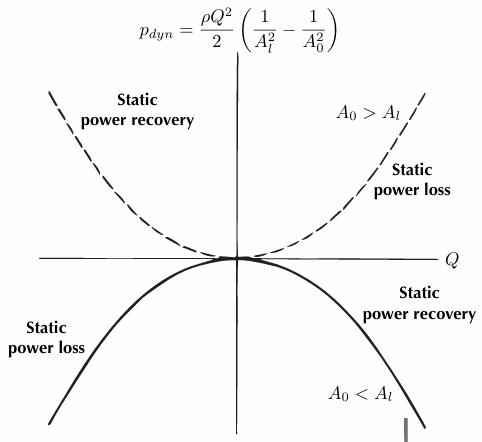
\includegraphics[width=0.4\textwidth]{figs/chapter8/8_6.png}
  \caption{The Bernoulli resistance characteristic}
\end{figure}


\subsection{Example: tank emptying through a pipe}
\label{ssec:tank_emptying}

To illustrate the utility of the bond-graph representation, consider
estimating the time for a \textbf{tank to empty through a pipe}.  The system
consists of a large tank (area $A_{T}$, volume $V$) connected to a pipe of
length $L$ and exit area $A_{2} \ll A_{1} \approx A_{T}$.  The pipe
discharges to a zero-pressure environment ($p_{L} = 0$).

The key assumption is that the fluid fills the pipe at all times ($v = Q/A$),
and the derived equations are valid for \emph{one direction of flow only}.

The bond-graph state equations, derived from~\eqref{eq:bernoulli_bg} with a
Bernoulli resistance and a fluid inertia $I = \rho L/A_{2}$, are:
\begin{align}
  \dot{V} &= -\frac{A_{2}}{\rho L}\,p_{p}, \qquad V \geq 0,
  \label{eq:tank_V}\\
  \dot{p}_{p} &= -\frac{\rho}{2A_{2}^{2}}\!\left(\frac{A_{2}}{\rho L}p_{p}\right)^{2}
  + \frac{\rho g V}{A_{T}}.
  \label{eq:tank_p}
\end{align}
Eliminating $p_{p}$ in favour of $V$:
\begin{equation}
  -\frac{\rho L}{A_{2}}\,\ddot{V}
  = -\frac{\rho}{2A_{2}^{2}}\,\dot{V}^{2} + \frac{\rho g}{A_{T}}\,V,
  \qquad V \geq 0.
  \label{eq:tank_ode}
\end{equation}
This is a second-order nonlinear ODE that can be integrated numerically.
Note that, although no static pressure power flows into the zero-pressure
source at the pipe exit, there \emph{is} a flow; with a diffuser at the
exit one could theoretically recover power from this flow.

\begin{figure}
  \centering
  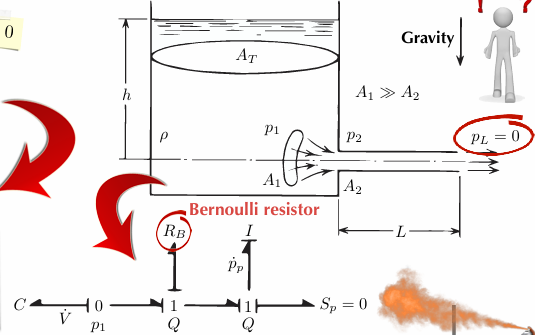
\includegraphics[width=0.4\textwidth]{figs/chapter8/8_7.png}
  \caption{Tank emptying}
\end{figure}


\subsection{Compressible fluids and the transition to pseudo-bond graphs}
\label{ssec:compressible}

For \textbf{small density changes} compressibility is readily modelled by
linear capacitors (as in~\eqref{eq:compliance}).  For
\textbf{large density changes} the thermodynamics of the fluid must be
studied explicitly.  Maintaining a true bond-graph representation for
compressible fluids leads to further complications; this fact motivates the
development of a new form of \textbf{pseudo-bond graph}.

The internal energy per unit mass depends on density $\rho$ and entropy $s$
through the Gibbs equation:
\begin{equation}
  \mathrm{d}u = T\,\mathrm{d}s - p\,\mathrm{d}\!\left(\frac{1}{\rho}\right),
  \qquad
  u = u\!\left(s, \frac{1}{\rho}\right),
  \label{eq:u_rho}
\end{equation}
where $1/\rho$ plays the role of specific volume.  This corresponds to a
C-field in the thermodynamic sense.  Using the C-field representation it is
straightforward to model \emph{closed} systems in which fixed amounts of a
fluid are compressed, expanded, and heated.  When the fluid
\textbf{passes into and out of a control volume} the situation is more
complex.


\subsection{Open volume: convection of internal energy}
\label{ssec:open_volume}

Consider a fluid compressed in a \textbf{fixed volume} $V_{0}$ by allowing
it to pass slowly in and out of a port with volumetric flow rate $Q$ and
pressure $p$:
\begin{equation}
  \rho = \frac{m}{V_{0}}, \qquad \dot{m} = \rho Q.
  \label{eq:open_density}
\end{equation}
The total energy $U$ in the control volume depends on the mass $m$ and the
internal energy per unit mass $u$.  Since $U$ changes not only because of
the \emph{flow work} $pQ$ but also because of the \emph{convection of
internal energy}, the correct flow variable is the \textbf{mass flow rate}
$\dot{m} = \rho Q$.  The energy balance is:
\begin{equation}
  \mathrm{d}U = u\,\mathrm{d}m + \frac{p}{\rho}\,\mathrm{d}m
  = h\,\mathrm{d}m,
  \qquad
  h = u + \frac{p}{\rho}
  \quad\text{(specific enthalpy)},
  \label{eq:dU_enthalpy}
\end{equation}
so that the power entering the control volume is:
\begin{equation}
  h\dot{m} = u\dot{m} + \frac{p}{\rho}\dot{m}
  = u\rho Q + \frac{p}{\rho}\,\rho Q
  = (\rho u + p)Q.
  \label{eq:enthalpy_power}
\end{equation}
In bond-graph terms, it is necessary to \textbf{supplement the pressure}
with an extra term $\rho u$ to account for the convected internal energy.
This is modelled by a \textbf{modulated transformer} (MTF) whose modulus is
$\rho$, converting the port $(p + \rho u,\, Q)$ to the port
$(h,\, \dot{m} = \rho Q)$, which then drives the C-field of the control
volume:

\begin{figure}
  \centering
  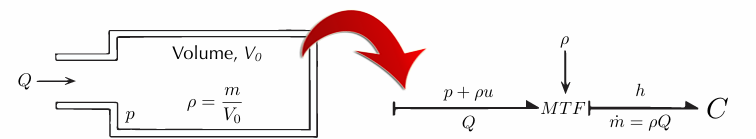
\includegraphics[width=1.0\textwidth]{figs/chapter8/8_8.png}
  \caption{Bond graph for a fixed-volume open control volume}
\end{figure}


\begin{insightbox}[Dynamic pressure neglected]
  The derivation above has \emph{not} incorporated the dynamic pressure term
  $\rho Q^{2}/(2A^{2})$.  The model is therefore valid only for low flow
  rates where the kinetic energy of the incoming stream is negligible
  compared to its enthalpy.
\end{insightbox}

In the \textbf{isentropic case} ($\dot{s} = 0$) pressure and internal
energy are determined solely by the density, so the enthalpy at the port is
determined entirely by conditions \emph{inside} the vessel.  In more
complicated cases (non-isentropic flow) the enthalpy at the port is
determined by:
\begin{itemize}[leftmargin=2em,itemsep=2pt]
  \item Conditions \emph{inside} the vessel for \emph{outflow}.
  \item \emph{External} conditions for \emph{inflow}.
\end{itemize}
This causal switching with changes in the direction of flow is not readily
apparent in the true bond graph; it will be explicitly addressed in the
pseudo-bond-graph formulations developed in the following chapters.


\subsection{Variable-volume compression: the piston--cylinder}
\label{ssec:piston_cylinder}

As a final extension, consider \textbf{isentropic compression} occurring
simultaneously due to variable volume (a piston) and to inflow/outflow.
The cylinder has area $A$, piston displacement $x$, and volume $V = Ax$.
The total energy $U$ depends on both the mass $m$ and the volume $V$, so
the C-field satisfies:
\begin{equation}
  h = \frac{\partial U}{\partial m},
  \qquad
  -p = \frac{\partial U}{\partial V}.
  \label{eq:piston_cfield}
\end{equation}
The bond graph is a more sophisticated version of the compressibility models
used in servomechanisms, where the volume of fluid is variable.

\begin{figure}
  \centering
  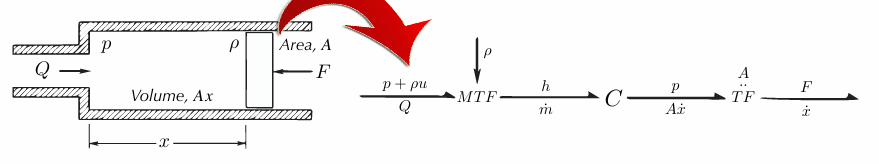
\includegraphics[width=1.0\textwidth]{figs/chapter8/8_9.png}
  \caption{Piston--cylinder with inflow/outflow}
\end{figure}

This bond graph is a powerful, general representation: it handles
simultaneously the thermodynamics of compression, the convection of mass and
energy through the port, and the mechanical work done by or on the piston.
Linearised compressibility parameters (constant bulk modulus) are a special
case, but it is \textbf{virtually impossible} to proceed from a linearised
model to a more accurate nonlinear one without returning to the physics and
reconstructing the bond graph from scratch.  The systematic derivation from
$U(m, V)$ ensures that the nonlinear model is available from the outset and
that no energy-conservation errors are introduced by \emph{ad hoc}
linearisation.

%──────────────────────────────────────────────────────────────────────
\section{Summary}
\label{sec:thermofluid_summary}
%──────────────────────────────────────────────────────────────────────

This chapter has developed the bond-graph treatment of thermo-fluid systems
at two levels of depth.

\paragraph{True bond graphs for thermodynamics.}
The pure substance is a 2-port C-field with $T$ (effort) and $\dot{s}$
(flow) at one port and $p$ (effort) and $\dot{v}$ (flow) at the other.  The
product $T\dot{s}$ is genuine thermodynamic power.  The four causal
patterns of this C-field correspond to the four classical thermodynamic
potentials ($u$, $h$, $f$, $\phi$) via Legendre transformations, and all
four automatically ensure conservation of energy.  Heat transfer is modelled
by a 2-port R-field that generates entropy; its only admissible causality
has temperatures as inputs.  A thermal I-element is physically impossible
(it would violate the second law).  With these elements a rich variety of
thermal and electrothermal systems can be modelled rigorously.

\paragraph{Fluid-dynamic lumped models.}
Standard lumped models of fluid systems (fluid inertia $I = \rho L/A$,
compliance $B/V_{0}$, friction $R$, leakage $R$) are useful for short,
linear elements but carry significant philosophical caveats for long pipes,
nonlinear flows, and compressible fluids.  The Bernoulli equation reveals
an unusual $Q^{2}$ term (dynamic pressure / Bernoulli resistance) that
can supply as well as dissipate power and creates multi-valuedness under
pressure-input causality.  For compressible fluids with mass exchange
through a control volume, the correct power variable at the port is the
enthalpy flux $h\dot{m}$, and the bond graph requires an MTF to account for
convected internal energy.  The resulting nonlinear C-field formulation is
the natural starting point for accurate models of pneumatic actuators,
compressors, and variable-volume reservoirs.

\end{document}